\documentclass[12pt, a4paper]{article}

% If you can't see cyrillic letters in R-studio choose
% File-Reopen with encoding
% utf8 is the preferred encoding


%%%%%%%%%%%%%%%%%%%%%%%  Загрузка пакетов  %%%%%%%%%%%%%%%%%%%%%%%%%%%%%%%%%%
% кусок от урсса
%\usepackage[60x90,headers,11pt]{format}

%\textheight=494pt%
%\textwidth=322pt%
%
%\oddsidemargin=0pt%
%\evensidemargin=0pt
%\topmargin=-1pt \headsep=14pt \headheight=22pt \voffset=-28pt
%\hoffset=-50pt


\clubpenalty=10000
\widowpenalty=10000

%\overfullrule=5pt
%\hfuzz=1.5mm
%\baselineskip=12pt plus 0.18pt minus 0.1pt


%\pagestyle{headings}
% конец куска от урсса




% специальная версия для knitr'а. Исключает graphicx

%\usepackage{showkeys} % показывать метки в готовом pdf

\usepackage{etex} % расширение классического tex
% в частности позволяет подгружать гораздо больше пакетов, чем мы и займёмся далее

%\usepackage{mathtext} % русские буквы в формулах? (и без неё работает)
% Например, $x_{\text{один}}$

%\usepackage{cmap} % для поиска русских слов в pdf --- теперь работает без этого
% а с cmap не работает печать на принтер ;)
\usepackage{verbatim} % для многострочных комментариев
\usepackage{makeidx} % для создания предметных указателей
\usepackage[X2, T2A]{fontenc}
\usepackage[utf8]{inputenc} % задание utf8 кодировки исходного tex файла
\usepackage{setspace}
\usepackage{amsmath, amsfonts, amssymb, amsthm}
\usepackage{mathrsfs} % sudo yum install texlive-rsfs
\usepackage{dsfont} % sudo yum install texlive-doublestroke
\usepackage{array, multicol, multirow, bigstrut} % sudo yum install texlive-multirow
\usepackage{indentfirst} % установка отступа в первом абзаце главы
\usepackage[russian]{babel} % выбор языка для документа
\usepackage{bm}
\usepackage{bbm} % шрифт с двойными буквами
%\usepackage[perpage]{footmisc}

\usepackage{dcolumn} % центрирование по разделителю для apsrtable

% создание гиперссылок в pdf
\usepackage[pdftex, unicode, colorlinks=true, urlcolor=blue, hyperindex, breaklinks]{hyperref}

% свешиваем пунктуацию
% теперь знаки пунктуации могут вылезать за правую границу текста, при этом текст выглядит ровнее
\usepackage{microtype}

\usepackage{textcomp}  % Чтобы в формулах можно было русские буквы писать через \text{}

% размер листа бумаги
%\usepackage[paperwidth=145mm,paperheight=215mm,
%height=182mm,width=113mm,top=20mm,includefoot]%{geometry}
\usepackage[paper=a4paper, top=15mm, bottom=13.5mm, left=16.5mm, right=13.5mm, includefoot]{geometry}

\usepackage{xcolor}

% \usepackage[pdftex]{graphicx} % для вставки графики, убрано, т.к. knitr похоже сам добавляет

\usepackage{float, longtable}
\usepackage{soulutf8}

\usepackage{enumitem} % дополнительные плюшки для списков
%  например \begin{enumerate}[resume] позволяет продолжить нумерацию в новом списке

\usepackage{mathtools}
\usepackage{cancel,xspace} % sudo yum install texlive-cancel

% \usepackage{minted} % display program code with syntax highlighting
% требует установки pygments и python

\usepackage{numprint} % sudo yum install texlive-numprint
\npthousandsep{,}\npthousandthpartsep{}\npdecimalsign{.}

\usepackage{embedfile} % Чтобы код LaTeXа включился как приложение в PDF-файл

\usepackage{subfigure} % для создания нескольких рисунков внутри одного

\usepackage{tikz, pgfplots} % язык для рисования графики из latex'a
\usetikzlibrary{trees} % tikz-прибамбас для рисовки деревьев
\usepackage{tikz-qtree} % альтернативный tikz-прибамбас для рисовки деревьев
\usetikzlibrary{arrows} % tikz-прибамбас для рисовки стрелочек подлиннее

\usepackage{forest} % деревья в tikz

\usepackage{todonotes} % для вставки в документ заметок о том, что осталось сделать
% \todo{Здесь надо коэффициенты исправить}
% \missingfigure{Здесь будет Последний день Помпеи}
% \listoftodos --- печатает все поставленные \todo'шки


% более красивые таблицы
\usepackage{booktabs}
% заповеди из докупентации:
% 1. Не используйте вертикальные линни
% 2. Не используйте двойные линии
% 3. Единицы измерения - в шапку таблицы
% 4. Не сокращайте .1 вместо 0.1
% 5. Повторяющееся значение повторяйте, а не говорите "то же"



%\usepackage{asymptote} % пакет для рисовки графики, должен идти после graphics
% но мы переходим на tikz :)

%\usepackage{sagetex} % для интеграции с Sage (вероятно тоже должен идти после graphics)

% metapost создает упрощенные eps файлы, которые можно напрямую включать в pdf
% эта группа команд декларирует, что файлы будут этого упрощенного формата
% если metapost не используется, то этот блок не нужен
\usepackage{ifpdf} % для определения, запускается ли pdflatex или просто латех
\ifpdf
    \DeclareGraphicsRule{*}{mps}{*}{}
\fi
%%%%%%%%%%%%%%%%%%%%%%%%%%%%%%%%%%%%%%%%%%%%%%%%%%%%%%%%%%%%%%%%%%%%%%


%%%%%%%%%%%%%%%%%%%%%%%  Внедрение tex исходников в pdf файл  %%%%%%%%%%%%%%%%%%%%%%%%%%%%%%%%%%
\embedfile[desc={Main tex file}]{\jobname.tex} % Включение кода в выходной файл
\embedfile[desc={title_bor}]{title_bor_utf8_knitr.tex}

%%%%%%%%%%%%%%%%%%%%%%%%%%%%%%%%%%%%%%%%%%%%%%%%%%%%%%%%%%%%%%%%%%%%%%



%%%%%%%%%%%%%%%%%%%%%%%  ПАРАМЕТРЫ  %%%%%%%%%%%%%%%%%%%%%%%%%%%%%%%%%%
\setstretch{1}                          % Межстрочный интервал
\flushbottom                            % Эта команда заставляет LaTeX чуть растягивать строки, чтобы получить идеально прямоугольную страницу
\righthyphenmin=2                       % Разрешение переноса двух и более символов
%\pagestyle{plain}                       % Нумерация страниц снизу по центру.
%\widowpenalty=300                     % Небольшое наказание за вдовствующую строку (одна строка абзаца на этой странице, остальное --- на следующей)
%\clubpenalty=3000                     % Приличное наказание за сиротствующую строку (омерзительно висящая одинокая строка в начале страницы)
\setlength{\parindent}{1.5em}           % Красная строка.
%\captiondelim{. }
\setlength{\topsep}{0pt}
%%%%%%%%%%%%%%%%%%%%%%%%%%%%%%%%%%%%%%%%%%%%%%%%%%%%%%%%%%%%%%%%%%%%%%



%%%%%%%% Это окружение, которое выравнивает по центру без отступа, как у простого center
\newenvironment{center*}{%
  \setlength\topsep{0pt}
  \setlength\parskip{0pt}
  \begin{center}
}{%
  \end{center}
}
%%%%%%%%%%%%%%%%%%%%%%%%%%%%%%%%%%%%%%%%%%%%%%%%%%%%%%%%%%%%%%%%%%%%%%


%%%%%%%%%%%%%%%%%%%%%%%%%%% Правила переноса  слов
\hyphenation{ }
%%%%%%%%%%%%%%%%%%%%%%%%%%%%%%%%%%%%%%%%%%%%%%%%%%%%%%%%%%%%%%%%%%%%%%

\emergencystretch=2em


% DEFS
\def \mbf{\mathbf}
\def \msf{\mathsf}
\def \mbb{\mathbb}
\def \tbf{\textbf}
\def \tsf{\textsf}
\def \ttt{\texttt}
\def \tbb{\textbb}

\def \wh{\widehat}
\def \wt{\widetilde}
\def \ni{\noindent}
\def \ol{\overline}
\def \cd{\cdot}
\def \fr{\frac}
\def \bs{\backslash}
\def \lims{\limits}
\DeclareMathOperator{\dist}{dist}
\DeclareMathOperator{\VC}{VCdim}
\DeclareMathOperator{\card}{card}
\DeclareMathOperator{\sign}{sign}
\DeclareMathOperator{\sgn}{sign}

\DeclareMathOperator{\Tr}{tr}
\DeclareMathOperator{\tr}{tr}
\DeclareMathOperator{\trace}{tr}

\def \xfs{(x_1,\ldots,x_{n-1})}
\DeclareMathOperator*{\argmin}{arg\,min}
\DeclareMathOperator*{\amn}{arg\,min}
\DeclareMathOperator*{\amx}{arg\,max}

\DeclareMathOperator{\rk}{rank}
\DeclareMathOperator{\rank}{rank}

\DeclareMathOperator{\grad}{grad}



\DeclareMathOperator{\Corr}{Corr}
\DeclareMathOperator{\sCorr}{sCorr}
\DeclareMathOperator{\sCov}{sCov}
\DeclareMathOperator{\sVar}{sVar}

\DeclareMathOperator{\Cov}{Cov}
\DeclareMathOperator{\Var}{Var}
\DeclareMathOperator{\corr}{Corr}
\DeclareMathOperator{\cov}{Cov}
\DeclareMathOperator{\var}{Var}
\DeclareMathOperator{\bin}{Bin}
\DeclareMathOperator{\Bin}{Bin}
\DeclareMathOperator{\rang}{rang}
\DeclareMathOperator*{\plim}{plim}
\DeclareMathOperator{\MSE}{MSE}

\providecommand{\iff}{\Leftrightarrow}
\providecommand{\hence}{\Rightarrow}

\def \ti{\tilde}
\def \wti{\widetilde}

\def \mA{\mathcal{A}}
\def \mB{\mathcal{B}}
\def \mC{\mathcal{C}}
\def \mE{\mathcal{E}}
\def \mF{\mathcal{F}}
\def \mH{\mathcal{H}}
\def \mL{\mathcal{L}}
\def \mN{\mathcal{N}}
\def \mU{\mathcal{U}}
\def \mV{\mathcal{V}}
\def \mW{\mathcal{W}}


\def \R{\mbb R}
\def \N{\mbb N}
\def \Z{\mbb Z}
\def \P{\mbb{P}}
\def \p{\mbb{P}}
\newcommand{\E}{\mathbb{E}}
\def \D{\msf{D}}
\def \I{\mbf{I}}

\def \QQ{\mbb Q}
\def \RR{\mbb R}
\def \NN{\mbb N}
\def \ZZ{\mbb Z}
\def \PP{\mbb P}


\def \a{\alpha}
\def \b{\beta}
\def \t{\tau}
\def \dt{\delta}
\newcommand{\e}{\varepsilon}
\def \ga{\gamma}
\def \kp{\varkappa}
\def \la{\lambda}
\def \sg{\sigma}
\def \sgm{\sigma}
\def \tt{\theta}
\def \ve{\varepsilon}
\def \Dt{\Delta}
\def \La{\Lambda}
\def \Sgm{\Sigma}
\def \Sg{\Sigma}
\def \Tt{\Theta}
\def \Om{\Omega}
\def \om{\omega}

%\newcommand{\p}{\partial}

\def \ni{\noindent}
\def \lq{\glqq}
\def \rq{\grqq}
\def \lbr{\linebreak}
\def \vsi{\vspace{0.1cm}}
\def \vsii{\vspace{0.2cm}}
\def \vsiii{\vspace{0.3cm}}
\def \vsiv{\vspace{0.4cm}}
\def \vsv{\vspace{0.5cm}}
\def \vsvi{\vspace{0.6cm}}
\def \vsvii{\vspace{0.7cm}}
\def \vsviii{\vspace{0.8cm}}
\def \vsix{\vspace{0.9cm}}
\def \VSI{\vspace{1cm}}
\def \VSII{\vspace{2cm}}
\def \VSIII{\vspace{3cm}}

\newcommand{\bls}[1]{\boldsymbol{#1}}
\newcommand{\bsA}{\boldsymbol{A}}
\newcommand{\bsH}{\boldsymbol{H}}
\newcommand{\bsI}{\boldsymbol{I}}
\newcommand{\bsP}{\boldsymbol{P}}
\newcommand{\bsR}{\boldsymbol{R}}
\newcommand{\bsS}{\boldsymbol{S}}
\newcommand{\bsX}{\boldsymbol{X}}
\newcommand{\bsY}{\boldsymbol{Y}}
\newcommand{\bsZ}{\boldsymbol{Z}}
\newcommand{\bse}{\boldsymbol{e}}
\newcommand{\bsq}{\boldsymbol{q}}
\newcommand{\bsy}{\boldsymbol{y}}
\newcommand{\bsbeta}{\boldsymbol{\beta}}
\newcommand{\fish}{\mathrm{F}}
\newcommand{\Fish}{\mathrm{F}}
\renewcommand{\phi}{\varphi}
\newcommand{\ind}{\mathds{1}}
\newcommand{\inds}[1]{\mathds{1}_{\{#1\}}}
\renewcommand{\to}{\rightarrow}
\newcommand{\sumin}{\sum\limits_{i=1}^n}
\newcommand{\ofbr}[1]{\bigl( \{ #1 \} \bigr)}     % Например, вероятность события. Большие круглые, нормальные фигурные скобки вокруг аргумента
\newcommand{\Ofbr}[1]{\Bigl( \bigl\{ #1 \bigr\} \Bigr)} % Например, вероятность события. Больше больших круглые, большие фигурные скобки вокруг аргумента
\newcommand{\oeq}{{}\textcircled{\raisebox{-0.4pt}{{}={}}}{}} % Равно в кружке
\newcommand{\og}{\textcircled{\raisebox{-0.4pt}{>}}}  % Знак больше в кружке

% вместо горизонтальной делаем косую черточку в нестрогих неравенствах
\renewcommand{\le}{\leqslant}
\renewcommand{\ge}{\geqslant}
\renewcommand{\leq}{\leqslant}
\renewcommand{\geq}{\geqslant}


\newcommand{\figb}[1]{\bigl\{ #1  \bigr\}} % большие фигурные скобки вокруг аргумента
\newcommand{\figB}[1]{\Bigl\{ #1  \Bigr\}} % Больше больших фигурные скобки вокруг аргумента
\newcommand{\parb}[1]{\bigl( #1  \bigr)}   % большие скобки вокруг аргумента
\newcommand{\parB}[1]{\Bigl( #1  \Bigr)}   % Больше больших круглые скобки вокруг аргумента
\newcommand{\parbb}[1]{\biggl( #1  \biggr)} % большие-большие круглые скобки вокруг аргумента
\newcommand{\br}[1]{\left( #1  \right)}    % круглые скобки, подгоняемые по размеру аргумента
\newcommand{\fbr}[1]{\left\{ #1  \right\}} % фигурные скобки, подгоняемые по размеру аргумента
\newcommand{\eqdef}{\mathrel{\stackrel{\rm def}=}} % знак равно по определению
\newcommand{\const}{\mathrm{const}}        % const прямым начертанием
\newcommand{\zdt}[1]{\textit{#1}}
\newcommand{\ENG}[1]{\foreignlanguage{british}{#1}}
\newcommand{\ENGs}{\selectlanguage{british}}
\newcommand{\RUSs}{\selectlanguage{russian}}
\newcommand{\iid}{\text{i.\hspace{1pt}i.\hspace{1pt}d.}}

\newdimen\theoremskip
\theoremskip=0pt
\newenvironment{note}{\par\vskip\theoremskip\textbf{Замечание.\xspace}}{\par\vskip\theoremskip}
\newenvironment{hint}{\par\vskip\theoremskip\textbf{Подсказка.\xspace}}{\par\vskip\theoremskip}
\newenvironment{ist}{\par\vskip\theoremskip Источник:\xspace}{\par\vskip\theoremskip}

\newcommand*{\tabvrulel}[1]{\multicolumn{1}{|c}{#1}}
\newcommand*{\tabvruler}[1]{\multicolumn{1}{c|}{#1}}

\newcommand{\II}{{\fontencoding{X2}\selectfont\CYRII}}   % I десятеричное (английская i неуместна)
\newcommand{\ii}{{\fontencoding{X2}\selectfont\cyrii}}   % i десятеричное
\newcommand{\EE}{{\fontencoding{X2}\selectfont\CYRYAT}}  % ЯТЬ
\newcommand{\ee}{{\fontencoding{X2}\selectfont\cyryat}}  % ять
\newcommand{\FF}{{\fontencoding{X2}\selectfont\CYROTLD}} % ФИТА
\newcommand{\ff}{{\fontencoding{X2}\selectfont\cyrotld}} % фита
\newcommand{\YY}{{\fontencoding{X2}\selectfont\CYRIZH}}  % ИЖИЦА
\newcommand{\yy}{{\fontencoding{X2}\selectfont\cyrizh}}  % ижица

%%%%%%%%%%%%%%%%%%%%% Определение разрядки разреженного текста и задание красивых многоточий
\sodef\so{}{.15em}{1em plus1em}{.3em plus.05em minus.05em}
\newcommand{\ldotst}{\so{...}}
\newcommand{\ldotsq}{\so{?\hbox{\hspace{-0.61ex}}..}}
\newcommand{\ldotse}{\so{!..}}
%%%%%%%%%%%%%%%%%%%%%%%%%%%%%%%%%%%%%%%%%%%%%%%%%%%%%%%%%%%%%%%%%%%%%%

%%%%%%%%%%%%%%%%%%%%%%%%%%%%% Команда для переноса символов бинарных операций
\def\hm#1{#1\nobreak\discretionary{}{\hbox{$#1$}}{}}
%%%%%%%%%%%%%%%%%%%%%%%%%%%%%%%%%%%%%%%%%%%%%%%%%%%%%%%%%%%%%%%%%%%%%%

%\setlist[enumerate,1]{label=\arabic*., ref=\arabic*, partopsep=0pt plus 2pt, topsep=0pt plus 1.5pt,itemsep=0pt plus .5pt,parsep=0pt plus .5pt}
%\setlist[itemize,1]{partopsep=0pt plus 2pt, topsep=0pt plus 1.5pt,itemsep=0pt plus .5pt,parsep=0pt plus .5pt}

% Эти парни затем, если вдруг не захочется управлять списками из-под уютненького enumitem
% или если будет жизненно важно, чтобы в списках были именно русские буквы.
%\setlength{\partopsep}{0pt plus 3pt}
%\setlength{\topsep}{0pt plus 2pt}
%\setlength{\itemsep}{0 plus 1pt}
%\setlength{\parsep}{0 plus 1pt}

%на всякий случай пока есть
%теоремы без нумерации и имени
%\newtheorem*{theor}{Теорема}

%"Определения","Замечания"
%и "Гипотезы" не нумеруются
%\newtheorem*{defin}{Определение}
%\newtheorem*{rem}{Замечание}
%\newtheorem*{conj}{Гипотеза}

%"Теоремы" и "Леммы" нумеруются
%по главам и согласованно м/у собой
%\newtheorem{theorem}{Теорема}
%\newtheorem{lemma}[theorem]{Лемма}

% Утверждения нумеруются по главам
% независимо от Лемм и Теорем
%\newtheorem{prop}{Утверждение}
%\newtheorem{cor}{Следствие}


\def \useR{$[$R$]$ }

%% эконометрические сокращения
\def \hb{\hat{\beta}}
\def \hs{\hat{s}}
\def \hy{\hat{y}}
\def \hY{\hat{Y}}
\def \he{\hat{\varepsilon}}
\def \v1{\vec{1}}
\def \e{\varepsilon}
\def \z{z}
\def \hVar{\widehat{\Var}}
\def \hCorr{\widehat{\Corr}}
\def \hCov{\widehat{\Cov}}


%% лаг
\renewcommand{\L}{\mathrm{L}}

%% алая и белая розы
%% запускается так: \WhiteRose[масштаб], например, \WhiteRose[0.5]
\newcommand{\WhiteRose}[1]{\begingroup
\setbox0=\hbox{\includegraphics[scale=#1]{/home/boris/science/econometrix/em301/roses/Yorkshire_rose.pdf}}%
\parbox{\wd0}{\box0}\endgroup}

\newcommand{\RedRose}[1]{\begingroup
\setbox0=\hbox{\includegraphics[scale=#1]{/home/boris/science/econometrix/em301/roses/Lancashire_rose.pdf}}%
\parbox{\wd0}{\box0}\endgroup}

\newcommand{\WhiteRoseLine}{
\begin{center}
\WhiteRose{0.3} Версия Белой Розы \WhiteRose{0.3}
\end{center}}

\newcommand{\RedRoseLine}{
\begin{center}
\RedRose{0.3} Версия Алой Розы \RedRose{0.3}
\end{center}}




\usepackage{minted}

\usepackage[bibencoding = auto, backend = biber,
sorting = none]{biblatex}

\addbibresource{mlearn_pro.bib}

\def \RR{\mathbb{R}}
\def \cN{\mathcal{N}}

\title{Заметки к семинарам по машинному обучению}
\author{Винни-Пух}
\date{\today}


% делаем короче интервал в списках
\setlength{\itemsep}{0pt}
\setlength{\parskip}{0pt}
\setlength{\parsep}{0pt}


\DeclareMathOperator{\Med}{Med}


\usepackage{answers}

%\newtheorem{problem}{Задача}
%\numberwithin{problem}{section}

\Newassociation{sol}{solution}{solution_file}
% sol --- имя окружения внутри задач
% solution --- имя окружения внутри solution_file
% solution_file --- имя файла в который будет идти запись решений
% можно изменить далее по ходу
\Opensolutionfile{solution_file}[all_solutions]
% в квадратных скобках фактическое имя файла



% магия для автоматических гиперссылок задача-решение
\newlist{myenum}{enumerate}{3}
% \newcounter{problem}[chapter] % нумерация задач внутри глав
\newcounter{problem}[section]

\newenvironment{problem}%
{%
\refstepcounter{problem}%
%  hyperlink to solution
     \hypertarget{problem:{\thesection.\theproblem}}{} % нумерация внутри глав
     % \hypertarget{problem:{\theproblem}}{}
     \Writetofile{solution_file}{\protect\hypertarget{soln:\thesection.\theproblem}{}}
     %\Writetofile{solution_file}{\protect\hypertarget{soln:\theproblem}{}}
     \begin{myenum}[label=\bfseries\protect\hyperlink{soln:\thesection.\theproblem}{\thesection.\theproblem},ref=\thesection.\theproblem]
     % \begin{myenum}[label=\bfseries\protect\hyperlink{soln:\theproblem}{\theproblem},ref=\theproblem]
     \item%
    }%
    {%
    \end{myenum}}
% для гиперссылок обратно надо переопределять окружение
% это происходит непосредственно перед подключением файла с решениями




\begin{document}

% \maketitle % ставим сюда название, автора и время создания

\section{Дифференциал}


Минитеория:

\begin{enumerate}
\item $d(XY) = dX \cdot Y +  X \cdot dY$
\item $dA = 0$
\item $d(X') = dX'$
\item $d\det X = \tr (...) $
\end{enumerate}



\begin{problem}
    Вспомним дифференциал :)
    \begin{enumerate}
        \item Известно, что $f(x) = x^2 + 3x$. Найдите $f'(x)$ и $df$. Чему равен $dx$ в точке $x=5$ при $dx=0.1$?
        \item Известно, что $f(x_1, x_2)=x_1^2 + 3x_1x_2^3$. Найдите $df$. Чему равен $df$ в точке $x_1=-2$, $x_2=1$ при $dx_1=0.1$ и $dx_2=-0.1$?
        \item Известно, что $F=\begin{pmatrix}
                5 & 6x_1 \\
                x_1x_2 & x_1^2x_2 \\
            \end{pmatrix}$. Найдите $dF$.
        \item Известно, что $F=\begin{pmatrix}
                7 & 8 & 9 \\
                2 & -1 & -2 \\
            \end{pmatrix}$. Найдите $dF$.
        \item Матрица $F$ имеет размер $2\times 2$, в строке $i$ столбце $j$ у неё находится элемент $f_{ij}$.
            Выпишите выражение $\tr(F'dF)$ в явном виде без матриц.
    \end{enumerate}
\begin{sol}
\end{sol}
\end{problem}


\begin{problem}
Пусть $t$ — скалярная переменная, $r$, $s$ — векторные переменные, $R$, $S$ — матричные переменные. Кроме того, $a$, $b$ — векторы констант, $A$, $B$ — матрицы констант.

Применив базовые правила дифференцирования найдите:
\begin{enumerate}
\item $d(ARB)$;
\item $d(r'r)$;
\item $d(r'Ar)$;
\item $d(R^{-1})$, воспользовавшись тем, что $R^{-1} \cdot R = I$;
\item $d \cos(r'r)$;
\item $d(r'Ar/r'r)$.
\end{enumerate}


\begin{sol}
\begin{enumerate}
\item $A(dR)B$
\item $2r'dr$
\item $r'(A'+A)dr$
\item $R^{-1}\cdot dR \cdot R^{-1}$
\item $-\sin(r'r)\cdot 2r'dr$
\item $\frac{r'(A'+A)dr \cdot r'r - r'Ar2r'dr}{(r'r)^2}$
\end{enumerate}
\end{sol}
\end{problem}


\begin{problem}
В методе наименьших квадратов минимизируется функция
\[
Q(\hb) = (y - X\hb)'(y - X\hb).
\]

\begin{enumerate}
\item Найдите $dQ(\hb)$ и $d^2Q(\hb)$;
\item Выпишите условия первого порядка для задачи МНК;
\item Выразите $\hb$ предполагая, что $X'X$ обратима.
\end{enumerate}


\begin{sol}
\begin{enumerate}
\item $dQ(\hb) = 2(y-X\hb)^T (-X) d\hb$, $d^2Q(\hb) = 2d\hb X^2 d\hb$
\item $dQ(\hb) = 0$
\item $\hb = (X^T X)^{-1} X^T y$
\end{enumerate}
\end{sol}
\end{problem}

\begin{problem}
В методе LASSO минимизируется функция
\[
Q(\hb) = (y - X\hb)'(y - X\hb) + \lambda \hb' \hb,
\]
где $\lambda$ — положительный параметр, штрафующий функцию за слишком большие значения $\hb$.

\begin{enumerate}
\item Найдите $dQ(\hb)$ и $d^2Q(\hb)$;
\item Выпишите условия первого порядка для задачи LASSO;
\item Выразите $\hb$.
\end{enumerate}

\begin{sol}
\begin{enumerate}
\item $dQ(\hb) = -2((y-X\hb)^T X + \lambda \hb^T) d\hb$, $d^2Q(\hb)=2d\hb^T(X^T X - \lambda I) d\hb$
\item $dQ(\hb) = 0$
\item $\hb = (X^T X - \lambda I)^{-1} X^T y$
\end{enumerate}
\end{sol}
\end{problem}



\begin{problem}

Пусть $A$ и $B$ — матрицы одного размера.
\begin{enumerate}
\item Докажите, что сумму $\sum_{ij} A_{ij} B_{ij}$ можно представить в виде $\tr(A'B)$.
\item Докажите, что $\tr(A'B) = \tr(AB') = \tr(B'A) = \tr(BA')$.
\end{enumerate}

\begin{sol}
\end{sol}
\end{problem}


\begin{problem}

Выведите формулу для $d\det X$.

\begin{sol}
\end{sol}
\end{problem}


\begin{problem}

Пусть $x_i$ — вектор-столбец $k\times 1$, $y_i$ — скаляр, равный $+1$ или $-1$, $\hb$ — вектор-столбец размера $k\times 1$. Рассмотрим функцию
\[
Q(\hb) = \sum_{i=1}^n \ln (1 + \exp(-y_ix_i'\hb)) + \lambda \hb' \hb
\]

\begin{enumerate}
\item Найдите $dQ$;
\item Найдите вектор-столбец $\grad Q$.
\end{enumerate}

\begin{sol}
\end{sol}
\end{problem}



\section{Линейная регрессия}

\begin{problem}
Рассмотрим задачу линейной регресии
\[
Q(w) = (y - Xw)^T(y - Xw) \to \min_{w}.
\]

\begin{enumerate}
\item Найдите $dQ(w)$ и $d^2Q(w)$.
\item Выведите формулу для оптимального $w$.
\item Выведите формулу для матрицы-шляпницы (hat-matrix), связывающей вектор фактических $y$ и вектор прогнозов $\hat y = H\cdot y$.
\end{enumerate}

\begin{sol}
\begin{enumerate}
\item $dQ(w) = 2(Xw - y)^T X dw$, $d^2Q(w) = 2 dw^T X^T X dw$
\item $w = (X^T X)^{-1} X^T y$
\item $\hat y = Xw = X (X^T X)^{-1} X^T y \Rightarrow H = X (X^T X)^{-1} X^T$
\end{enumerate}
\end{sol}
\end{problem}

\begin{problem}
Рассмотрим задачу регрессии с одним признаком и без константы, $\hy_i = w \cdot x_i$. Решите в явном виде задачи МНК со штрафом:

\begin{enumerate}
\item $Q(w) = (y - \hy)^T (y - \hy) + \lambda w^2$;
\item $Q(w) = (y - \hy)^T (y - \hy) + \lambda |w|$;
\end{enumerate}

\begin{sol}
\begin{enumerate}
\item Выпишем $dQ(W)$ и найдём градиент:
\[ dQ(w) = 2(Xw - y)^T X dw + 2 \lambda w^T dw \Rightarrow \nabla Q (w) = 2 X^T (Xw - y) + 2 \lambda w \]
Приравняв градиент к нулю, получим:
\[w = (X^T X + \lambda I)^{-1} X^T y \]
\item
\end{enumerate}
\end{sol}
\end{problem}

\begin{problem}
Храбрая и торопливая исследовательница Мишель хочет решить задачу линейной регрессии по $n$ наблюдениям с вектором $y$ и матрицей признаков $X$. Сначала исследовательница Мишель так торопилась, что совсем забыла последнее наблюдение и оценила задачу с более коротким вектором $y^{-}$ и матрицей $X^{-}$, где не хватает последней строки. Затем Мишель взяла правильную матрицу $X$, но неправильный вектор $y^*$, в котором она вместо фактического последнего наблюдения вектора $y$ вписала его прогноз, полученный с помощью регрессии с $y^{-1}$ и $X^{-}$.

\begin{enumerate}
\item Как связаны $\hat y_n^{-}$ и $\hat y_n^{*}$ (прогнозы для последнего наблюдения полученные по модели без последнего наблюдения и модели с неверным последним наблюдением)?
\item Как выглядит вектор, равный разнице $y - y^*$?
\item Какие величины находятся в векторе $H\cdot (y - y^*)$? Чему равна последняя, $n$-ая, компонента этого вектора? Выразите её через $H_{nn}$ и ошибку прогноза последнего наблюдения по модели без последнего наблюдения, $y_n - \hat y_n^{-}$.
\item Как связаны между собой ошибка прогноза $n$-го наблюдения по полной модели, ошибка прогноза $n$-го наблюдения по модели без последнего наблюдения и $H_{nn}$?
\item Как быстро провести кросс-валидацию с выкидыванием одного наблюдения для задачи линейной регрессии?
\end{enumerate}

\begin{sol}
\[
y_n - \hat y_n = (1 - H_{nn}) (y_n - \hat y_n^-)
\]
\end{sol}
\end{problem}


\section{Линейные классификаторы}

\begin{problem}
Рассмотрим плоскость в $\RR^3$, задаваемую уравнением $5x_1 + 6x_2 -7x_3 + 10 = 0$ и две точки, $A = (2, 1, 4)$ и $B = (4, 0, 4)$.
\begin{enumerate}
  \item Найдите любой вектор, перпендикулярный плоскости.
  \item Правда ли, что отрезок $AB$ пересекает плоскость?
  \item Найдите длину отрезка $AB$;
  \item Не находя расстояние от точек до плоскости, определите, во сколько раз точка $A$ дальше от плоскости, чем точка $B$;
  \item Найдите расстояние от точки $A$ до плоскости.
\end{enumerate}

\begin{sol}
  \begin{enumerate}
  \item $(5, 6, -7)$
  \item Подставим точки $A$ и $B$ в уравнение плоскости:
  \[A: 5 \cdot 2 + 6 \cdot 1 - 7 \cdot 4 + 10 = -2 \]
  \[B: 5 \cdot 4 + 6 \cdot 0 - 7 \cdot 4 + 10 = 2 \]
  Точки $A$ и $B$ лежат по разные стороны плоскости, следовательно, отрезок $AB$ пересекает её.
  \item $\overrightarrow{AB} = (2, -1, 0)$, $|AB| = \sqrt{4 + 1 + 0} = \sqrt{5}$
  \item Расстояние одинаково % на семинаре условие было изменено
  \item $\rho = \frac{|5 \cdot 2 + 6 \cdot 1 - 7 \cdot 4 + 10|}{\sqrt{5^2 + 6^2 + 7^2}} = \frac{2}{\sqrt{10}}$
  \end{enumerate}
\end{sol}
\end{problem}


\begin{problem}
Рассмотрим простейший персептрон с константой, единственным входом $x_1$ и пороговой функцией активации. Подберите веса так, чтобы персептрон реализовывал логическое отрицание (в ответ на 0 выдавал 1, и наоборот).
\begin{sol}
Например, $w_1 = -2$, $w_0 = 2$, где $w_0$ — вес при константе.
\end{sol}
\end{problem}

\begin{problem}
Рассмотрим простейший персептрон с константой, двумя входами $x_1$, $x_2$ и пороговой функцией активации.

\todo[inline]{Здесь ассистенты нарисуют в tikz картинку, достойную стоять вместо Джоконды в Лувре}

\begin{enumerate}
\item Подберите веса так, чтобы персептрон реализовывал логическое ИЛИ (OR).
\item Подберите веса так, чтобы персептрон реализовывал логическое И (AND).
\item Докажите, что веса невозможно подобрать так, чтобы персептрон реализовывал исключающее логическое ИЛИ (XOR).
\item Добавьте персептрону вход $x_3 = x_1 \cdot x_2$ и подберите веса так, чтобы персептрон реализовывал XOR.
\item Реализуйте XOR с помощью трёх персептронов с двумя входами и константой. Укажите веса и схему их взаимосвязей.
\end{enumerate}

\begin{sol}
\begin{enumerate}
\item Например, $w_1 = 2, w_2 = 2, w_0 = 0$
\item Например, $w_1 = 2, w_2 = 2, w_0 = -2$
\item Можно показать графически: нарисовать на плоскости точки $(0,0), (1,1), (1,0), (0,1)$, причём для первых двух
нейрон должен выдавать ответ $0$, а для вторых — $1$. Чтобы разделить эти точки, необходимо провести две прямые,
в то время как один нейрон проводит только одну.
\item Например, подойдут веса $w_1 = 3, w_2 = 3, w_3 = -5, w_0 = -1$
\item Первый нейрон с весами $w_{11} = 1, w_{12} = 1, w_{10} = 1/2$ и второй нейрон с весами $w_{21} = 1, w_{22} = 1, w_{10} = -1/2$
должны подавать реузльтаты на вход третьему нейрону с весами $w_{31} = 3, w_{32} = -1, w_{30} = -2$
\end{enumerate}
\end{sol}
\end{problem}



\begin{problem}
В коробке завалялось три персептрона, у каждого два входа с константой и пороговая функция активации. Реализуйте с их помощью функцию
\[
y = \begin{cases}
1, \text{ если } x_2 \geq |x_1 - 3| + 2; \\
0, \text{ иначе}
\end{cases}.
\]
\begin{sol}
\end{sol}
\end{problem}



\begin{problem}
Рассмотрим следующий набор данных:

\begin{tabular}{ccc}
\toprule
$x_i$ & $z_i$ & $y_i$ \\
\midrule
-1 & -1 & 0 \\
1 & -1 & 0 \\
-1 & 1 & 0 \\
1 & 1 & 0 \\
0 & 2 & 1 \\
2 & 0 & 1 \\
0 & -2 & 1 \\
-2 & 0 & 1 \\
\bottomrule
\end{tabular}

\begin{enumerate}
\item Существует ли перспетрон с константой, двумя входами и пороговой функцией активации, способный идеально классифицировать $y_i$ на данной выборке? А хватит ли двух таких персептронов? А может хватит трёх?
\item Введите такое преобразование исходных признаков $h_i = h(x_i, z_i)$, при котором с идеальной классификацией $y_i$ справился бы даже персептрон с одним входом, константой и пороговой функцией активации.
\end{enumerate}


\begin{sol}
\end{sol}
\end{problem}





\begin{problem}
Бандерлог из Лога\footnote{деревня в Кадуйском районе Вологодской области} ведёт блог, любит считать логарифмы и оценивать логистические регрессии. С помощью нового алгоритма Бандерлог решил задачу классификации по трём наблюдениям и получил $b_i = \hat\P(y_i = 1|x_i)$.

\begin{tabular}{cc}
  \toprule
  $y_i$ & $b_i$ \\
  \midrule
  1 & 0.7 \\
  -1 & 0.2 \\
  -1 & 0.3 \\
  \bottomrule
\end{tabular}

\begin{enumerate}
\item Постройте ROC-кривую.
\item Найдите площадь под ROC-кривой и индекс Джини.
\item Постройте PR-кривую (кривая точность-полнота).
\item Найдите площадь под PR-кривой.
\item Как по-английски будет «бревно»?
\end{enumerate}
\begin{sol}
\end{sol}
\end{problem}



\begin{problem}
Классификатор Бандерлога имеет вид
\[
a_i = \begin{cases}
1, \text{ если } b_i > t; \\
-1, \text{ иначе.}
\end{cases}
\]

Докажите, что площадь под ROC-кривой равна вероятности того, случайно выбранный положительный объект окажется позже случайно выбранного отрицательного объекта, если объекты ранжированы по возрастанию величины $b_i$.
\begin{sol}
\end{sol}
\end{problem}






\begin{problem}
Все средние издалека выглядят одинаково, $\text{среднее}=f^{-1}(0.5f(x_1) + 0.5f(x_2))$.  Например, у среднего арифметического $f(t)=t$, у среднего гармонического $f(t)=1/t$.

\begin{enumerate}
  \item Какая $f$ используется для среднего геометрического?
\end{enumerate}

Для измерения качества бинарной классификации Ара использует среднее арифметическое точности и полноты, Гена — среднее геометрическое, а Гарик — среднее гармоническое.

\begin{enumerate}[resume]
  \item У кого будут выходить самые «качественные» и самые «некачественные» прогнозы?
\end{enumerate}


\begin{sol}
\begin{enumerate}
\item $f(t) = \log(t)$
\item Среднее гармоническое < среднее геометрическое < среднее арифметическое
\end{enumerate}
\end{sol}
\end{problem}


\begin{problem}
Бандерлог начинает все определения со слов «это доля правильных ответов»:
\begin{enumerate}
  \item accuracy — это доля правильных ответов\ldots
  \item точность (precision) — это доля правильных ответов\ldots
  \item полнота (recall) — это доля правильных ответов\ldots
  \item TPR — это доля правильных ответов\ldots
\end{enumerate}

Закончите определения Бандерлога так, чтобы они были, хм, правильными.
\begin{sol}
\begin{enumerate}
\item $\text{accuracy} = \frac{\text{TP} + \text{TN}}{\text{TP} +\text{FP} +\text{FN} +\text{TN}}$
\item $\text{precision} = \frac{\text{TP}}{\text{TP} +\text{FP}}$
\item $\text{recall} = \frac{\text{TP}}{\text{TP} +\text{FN}}$
\item $\text{TPR} = \frac{\text{TP}}{\text{TP} +\text{FN}}$
\end{enumerate}
\end{sol}
\end{problem}


\begin{problem}
Алгоритм бинарной классификации, придуманный Бандерлогом, выдаёт оценки вероятности $b_i = \hat\P(y_i=1 | x_i)$. Всего у Бандерлога 10000 наблюдений. Если ранжировать их по возрастанию $b_i$, то окажется что наблюдения с $y_i = 1$ занимают ровно места с  5501 по 5600.

Найдите площадь по ROC-кривой и площадь под PR-кривой.
\begin{sol}
\end{sol}
\end{problem}



\begin{problem}
Бандерлог собрал выборку из 900 муравьёв и 100 китов. Переменная $y_i$ равна $1$ для китов. Бандерлог хочет, чтобы его алгоритм классификации выдавал для каждого наблюдения число $b_i=f(x_i) \in [0;1]$, оценку вероятности того, что наблюдение является китом. В качестве признака Бандерлог использует количество глаз, не задумавшись о том, что оно равно двум и для муравьёв, и для китов.

Решите задачу минимизации эмпирической функции риска и найдите все $b_i$ для функций потерь:
\begin{enumerate}
  \item $L(y_i, b_i) = (y_i - b_i)^2$, если для муравьёв $y_i = 0$;
  \item $L(y_i, b_i) = |y_i - b_i|$, если для муравьёв $y_i = 0$;
  \item $L(y_i, b_i) = \begin{cases}
  -\log b_i, \text{ если } y_i = 1 \\
  -\log (1-b_i), \text{ иначе.}
  \end{cases}$;
  %\item $L(y_i, b_i) = \log (1 + \exp(-y \cdot b))$, если для муравьёв $y = -1$;
  \item $L(y_i, b_i) = \begin{cases}
  1/b_i, \text{ если } y_i = 1 \\
  1/(1-b_i), \text{ иначе.}
  \end{cases}$;
\end{enumerate}
\begin{sol}
\begin{enumerate}
\item Поскольку все признаки одинаковы, то $\forall i \quad b_i = f(x_i) = b$, и функционал ошибки иммет вид:
\[Q(b) = \frac{1}{1000} \sum_{i=1}^{1000} L(y_i, b) = \frac{1}{1000} \left(\sum_{i=1}^{900} b^2 + \sum_{i=1}^{100} (1-b)^2\right) \to \min_{b} \]
Дифференцируем и находим $b$:
\[2 \cdot 900 \cdot b - 2 \cdot 100 \cdot (1-b) = 0 \Rightarrow b = 0.1 \]
\item Аналогично:
\[Q(b) =  \frac{1}{1000} \sum_{i=1}^{1000} |y_i - b| = \frac{1}{1000} \left(900 \cdot b + 100|1-b| \right) \to \min_{b} \]
При $b=1$, получаем: $Q(1) = 0.9$
При $b<1$: $Q(b) = \frac{1}{1000} \left(900b + 100 - 100b \right) = \frac{1}{1000} \left(900b+100 \right)\to \min_{b}$.
Минимум функционала ошибки достигается при $b=0$ и равен $0.1$.
\item Снова выпишем функционал ошибки:
\[Q(b) = \frac{1}{1000} \left(-900 \log(1-b) + 100 \log b  \right) \to \min_b \]
Берём производную и получаем оптимальный $b$:
\[\frac{1}{1000} \left(\frac{900}{1-b} - \frac{100}{b} \right) = 0 \Rightarrow b = 0.1 \]
\item \[Q(b) = \frac{1}{1000} \left(\frac{900}{1-b} - \frac{100}{b} \right) \to \min_b  \]
Дифференцируя, получим:
\[\frac{900}{(1-b)^2} =  \frac{100}{b^2} \Rightarrow b = 0.25 \]
\end{enumerate}
\end{sol}
\end{problem}


\begin{problem}
Бандерлог утверждает, что открыл новую верхнюю границу для пороговой функции потерь, $\tilde{L}(M_i) = 1 + \frac{1}{\pi} \cdot \arctan(-x_i)$, где $M_i = y_i \cdot \langle w, x_i \rangle$. Прав ли бандерлог?
\begin{sol}
  Нет. Не выполнено $\tilde{L} \geq L$ для всех $M \in \RR$.
\end{sol}
\end{problem}


\begin{problem}
Бандерлог из Лога оценил логистическую регрессию по четырём наблюдениям и одному признаку с константой, получил $b_i = \hat\P(y_i = 1|x_i)$, но потерял последнее наблюдение:

\begin{tabular}{cc}
  \toprule
  $y_i$ & $b_i$ \\
  \midrule
  1 & 0.7 \\
  -1 & 0.2 \\
  -1 & 0.3 \\
  ? &  ? \\
  \bottomrule
\end{tabular}

\begin{enumerate}
\item Выпишите функцию потерь для задачи логистической регрессии.
\item Выпишите условие первого порядка по коэффициенту перед константой.
\item Помогите бандерлогу восстановить пропущенные значения!
\end{enumerate}

\begin{sol}
\end{sol}
\end{problem}


\begin{problem}
У Бандерлога три наблюдения, первое наблюдение — кит, остальные — муравьи. Киты кодируются $y_i = 1$, муравьи — $y_i = -1$. На этот раз Бандерлог, чтобы быть уверенным, что $x_i$ различаются, сам лично определил $x_i = i$. После этого Бандерлог оценивает логистическую регрессию с константой.

\begin{enumerate}
  \item Выпишите эмпирическую функцию риска, которую минимизирует Бандерлог;
  \item При каких оценках коэффициентов логистической регрессии эта функция достигает своего минимума?
\end{enumerate}

\begin{sol}
\end{sol}
\end{problem}

\begin{problem}
Рассмотрим целевую функцию логистической регрессии с константой
\[
Q(w) = \frac{1}{\ell} \sum L(y_i, b_i),
\]
где $b_i = 1 / (1 + \exp( -\langle w, x_i\rangle)$ и $L(y_i, b_i) = \begin{cases}
-\log b_i, \text{ если } y_i = 1 \\
-\log (1-b_i), \text{ иначе.}
\end{cases}$.

\begin{enumerate}
\item Найдите $dQ(w)$ и $d^2Q(w)$;
\item Найдите $dQ(0)$ и $d^2Q(0)$;
\item Выпишите квадратичную аппроксимацию для $Q(w)$ в окрестности $w=0$;
\item С какой задачей совпадает задача минимизации квадратичной аппроксимации?
\end{enumerate}

\begin{sol}
\end{sol}
\end{problem}



\begin{problem}
Винни-Пух знает, что мёд бывает правильный, $honey_i=1$, и неправильный, $honey_i=0$. Пчёлы также бывают правильные, $bee_i=1$, и неправильные, $bee_i=0$. По 100 своим попыткам добыть мёд Винни-Пух составил таблицу сопряженности:

\begin{tabular}{c|cc}
\toprule
 & $honey_i=1$ & $honey_i=0$ \\
\midrule
$bee_i=1$ & 12 & 36 \\
$bee_i=0$ & 32 & 20 \\
\bottomrule
\end{tabular}

Винни-Пух использует логистическую регрессию с константой для прогнозирования правильности мёда с помощью правильности пчёл.

\begin{enumerate}
\item Какие оценки коэффициентов получит Винни-Пух?
\item Какой прогноз вероятности правильности мёда при встрече с неправильными пчёлами даёт логистическая модель? Как это число можно посчитать без рассчитывания коэффициентов?
\end{enumerate}

\begin{sol}
\end{sol}
\end{problem}


\begin{problem}
Винни-Пух оценил логистическую регрессию для прогнозирования правильности мёда от высоты дерева (м) $x_i$ и удалённости от дома (км) $z_i$: $\ln odds_i = 2+0.3x_i - 0.5z_i$.
\begin{enumerate}
\item Оцените вероятность того, что $y_i=1$ для $x=15$, $z=3.5$.
\item Оцените предельный эффект увеличения $x$ на единицу на вероятность того, что $y_i=1$ для $x=15$, $z=3.5$.
\item При каком значении $x$ предельный эффект увеличения $x$ на единицу в точке $z=3.5$ будет максимальным?
\end{enumerate}

\begin{sol}
Предельный эффект максимален при максимальной производной $\Lambda'(\hat \beta_1 + \hat\beta_2x + \hat\beta_3z)$, то есть при $\hat \beta_1 + \hat\beta_2x + \hat\beta_3z=0$.
\end{sol}
\end{problem}

% \section{Хочу ещё задач!}



\section{Матрицы}


\begin{problem}
Известна матрица $X$,
\[
X = \begin{pmatrix}
1 & 1 \\
0 & 1 \\
-1 & 0 \\
\end{pmatrix};
\]

\begin{enumerate}
\item Найдите QR-разложение матрицы $X'X$;
\item Найдите QR-разложение матрицы $XX'$;
\item Найдите спектральное разложение матрицы $X'X$;
\item Найдите спектральное разложение матрицы $XX'$;
\item Найдите сингулярное разложение (SVD) матрицы $X$;
\end{enumerate}

\begin{sol}

\end{sol}
\end{problem}


\begin{problem}
Объясните геометрический смысл QR, SVD и спектрального разложений.
\begin{sol}
\end{sol}
\end{problem}



\begin{problem}
Бандрелог выполнил SVD-разложение матрицы регрессоров $X$. Помогите Бандерлогу поскорее найти формулу для матрицы-шляпницы $H$, которая проецирует $y$ на пространство столбцов матрицы $X$, $\hat y = Hy$.
\begin{sol}
\end{sol}
\end{problem}




\begin{problem}
Бандрелог выполнил QR-разложение матрицы регрессоров $X$. Помогите Бандерлогу поскорее найти формулу для матрицы-шляпницы $H$, которая проецирует $y$ на пространство столбцов матрицы $X$, $\hat y = Hy$.
\begin{sol}
\end{sol}
\end{problem}

\section{Метод опорных векторов}



\begin{problem}
На плоскости имеются точки двух цветов. Красные: $(1,1)$, $(1,-1)$ и синие: $(-1,1)$, $(-1,-1)$.
\begin{enumerate}
\item Найдите разделяющую гиперплоскость методом опорных векторов при разных $C$.
\item Укажите опорные вектора.
\end{enumerate}



\begin{sol}
\end{sol}
\end{problem}


\begin{problem}
На плоскости имеются точки двух цветов. Красные: $(1,1)$, $(1,-1)$ и синие: $(-1,1)$, $(-1,-1)$ и $(2,0)$.
\begin{enumerate}
\item Найдите разделяющую гиперплоскость методом опорных векторов при разных $C$.
\item Укажите опорные вектора.
\end{enumerate}



\begin{sol}
\end{sol}
\end{problem}




\begin{problem}
Эконометресса Авдотья решила использовать метод опорных векторов с гауссовским ядром с параметром $\sigma=1$ и штрафным коэффициентом $C=1$. Соответственно, она минимизировала целевую функцию

\[
\frac{w'w}{2} + C\sum_{i=1}^n \xi_i,
\]

где разделяющая плоскость задаётся $w'x-w_0=0$, а $\xi_i$ — размеры «заступа» за разделяющую полосу.

Затем Автдотья подумала, что неплохо бы выбрать наилучшие $C$ и $\sigma$. Ей лень было использовать кросс-валидацию, поэтому Авдотья минимизировала данную функцию по $C\geq 0$ и $\sigma\geq 0$. Какие значения она получила?


\begin{sol}
$C=0$ и $\sigma=+\infty$
\end{sol}
\end{problem}


\begin{problem}
Задан вектор $w=(2,3)$ и число $w_0=7$.

\begin{enumerate}
\item Нарисуйте прямые $\langle w, x\rangle=w_0$, $\langle w, x\rangle=w_0+1$, $\langle w, x\rangle=w_0-1$.
\item Найдите ширину полосы между $\langle w, x\rangle=w_0+1$ и $\langle w, x\rangle=w_0-1$.
\item Найдите расстояние от точки $(5,6)$ до прямой $\langle w, x\rangle=w_0-1$.
\end{enumerate}

\begin{sol}
\end{sol}
\end{problem}


\begin{problem}
Заданы две прямые, $l_0$: $x^{(1)}+3x^{(2)} = 9$ и $l_1$: $x^{(1)}+3x^{(2)} = 13$. Найдите подходяющий вектор $w$ и число $w_0$ так, чтобы прямая $l_0$ записывалась как  $\langle w,x \rangle=w_0-1$, а прямая $l_1$ как  $\langle w,x\rangle=w_0 + 1$.
\begin{sol}
\end{sol}
\end{problem}


\begin{problem}
Даны наблюдения

\begin{tabular}{ccc}
 $x^{(1)}$ & $x^{(2)}$ & $y$ \\
\midrule
 1 & 0 & 0 \\
 2 & 0 & 0 \\
 0 & 3 & 1 \\
 0 & 4 & 1 \\
\end{tabular}

\begin{enumerate}
\item Нарисуйте разделяющую полосу наибольшей ширины.
\item Решите задачу оптимизации
\[
\min_{w, w_0} \frac{1}{2} \langle w, w \rangle
\]

при ограничении: для $y_i=1$ выполнено условие $\langle w,x \rangle \geq w_0 + 1$, а для $y_i=0$ выполнено условие $\langle w,x \rangle \leq w_0 - 1$.
\item Для точки $x=(x^{(1)}, x^{(2)}) =(1, 1)$ найдите значение $\langle w,x \rangle-w_0$ и постройте прогноз $\hy$.
\end{enumerate}

\begin{sol}
\end{sol}
\end{problem}

\begin{problem}

По картинке качественно решите задачу разделения точек:



\begin{minipage}{0.6\textwidth}
\begin{center}
%\begin{tikzpicture}[scale = 0.025]
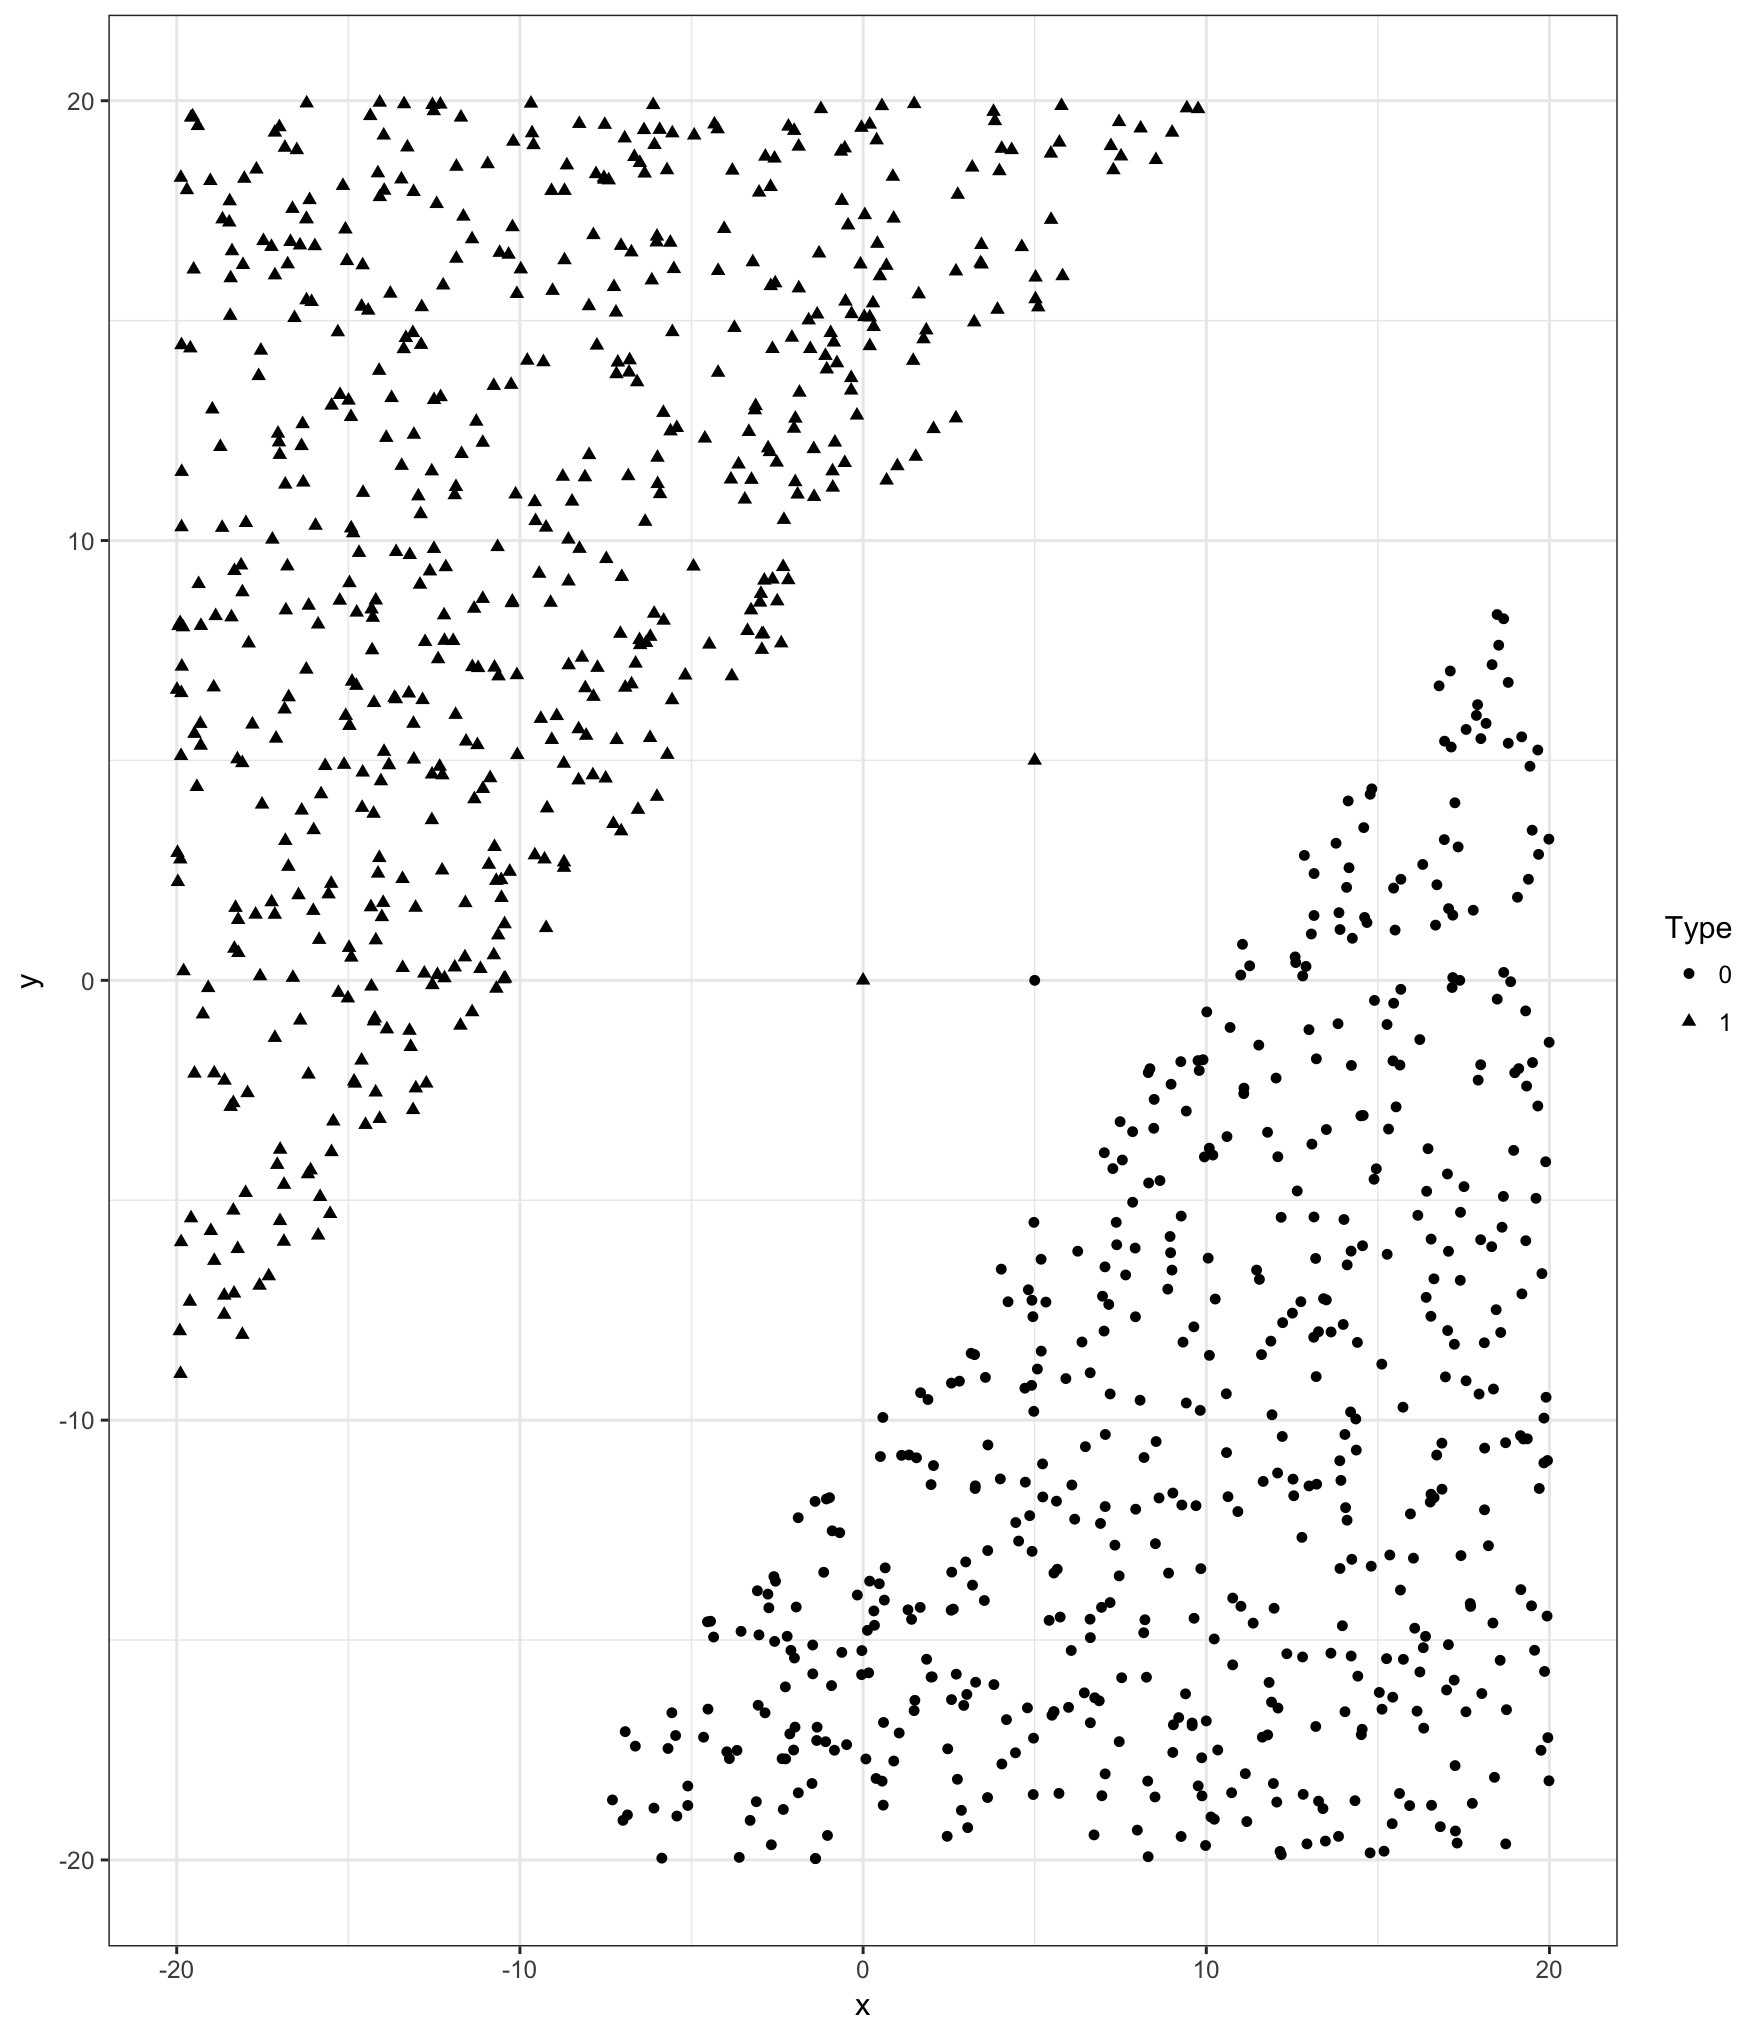
\includegraphics[scale=0.2]{images/armada.png}
%% Created by tikzDevice version 0.10.1 on 2017-09-29 08:31:35
% !TEX encoding = UTF-8 Unicode
\definecolor{fillColor}{RGB}{255,255,255}
\path[use as bounding box,fill=fillColor,fill opacity=0.00] (0,0) rectangle (505.89,505.89);
\begin{scope}
\path[clip] (  0.00,  0.00) rectangle (505.89,505.89);
\definecolor{drawColor}{RGB}{255,255,255}
\definecolor{fillColor}{RGB}{255,255,255}

\path[draw=drawColor,line width= 0.6pt,line join=round,line cap=round,fill=fillColor] (  0.00,  0.00) rectangle (505.89,505.89);
\end{scope}
\begin{scope}
\path[clip] ( 37.20, 29.59) rectangle (452.88,500.39);
\definecolor{fillColor}{RGB}{255,255,255}

\path[fill=fillColor] ( 37.20, 29.59) rectangle (452.88,500.39);
\definecolor{drawColor}{gray}{0.92}

\path[draw=drawColor,line width= 0.3pt,line join=round] ( 37.20,103.87) --
	(452.88,103.87);

\path[draw=drawColor,line width= 0.3pt,line join=round] ( 37.20,211.25) --
	(452.88,211.25);

\path[draw=drawColor,line width= 0.3pt,line join=round] ( 37.20,318.62) --
	(452.88,318.62);

\path[draw=drawColor,line width= 0.3pt,line join=round] ( 37.20,425.99) --
	(452.88,425.99);

\path[draw=drawColor,line width= 0.3pt,line join=round] (103.38, 29.59) --
	(103.38,500.39);

\path[draw=drawColor,line width= 0.3pt,line join=round] (197.96, 29.59) --
	(197.96,500.39);

\path[draw=drawColor,line width= 0.3pt,line join=round] (292.54, 29.59) --
	(292.54,500.39);

\path[draw=drawColor,line width= 0.3pt,line join=round] (387.13, 29.59) --
	(387.13,500.39);

\path[draw=drawColor,line width= 0.6pt,line join=round] ( 37.20, 50.19) --
	(452.88, 50.19);

\path[draw=drawColor,line width= 0.6pt,line join=round] ( 37.20,157.56) --
	(452.88,157.56);

\path[draw=drawColor,line width= 0.6pt,line join=round] ( 37.20,264.93) --
	(452.88,264.93);

\path[draw=drawColor,line width= 0.6pt,line join=round] ( 37.20,372.31) --
	(452.88,372.31);

\path[draw=drawColor,line width= 0.6pt,line join=round] ( 37.20,479.68) --
	(452.88,479.68);

\path[draw=drawColor,line width= 0.6pt,line join=round] ( 56.09, 29.59) --
	( 56.09,500.39);

\path[draw=drawColor,line width= 0.6pt,line join=round] (150.67, 29.59) --
	(150.67,500.39);

\path[draw=drawColor,line width= 0.6pt,line join=round] (245.25, 29.59) --
	(245.25,500.39);

\path[draw=drawColor,line width= 0.6pt,line join=round] (339.83, 29.59) --
	(339.83,500.39);

\path[draw=drawColor,line width= 0.6pt,line join=round] (434.42, 29.59) --
	(434.42,500.39);
\definecolor{fillColor}{RGB}{0,0,0}

\path[fill=fillColor] (390.23, 60.98) circle (  1.96);

\path[fill=fillColor] (243.49,384.30) --
	(246.14,379.72) --
	(240.85,379.72) --
	cycle;

\path[fill=fillColor] (122.12,458.91) --
	(124.76,454.33) --
	(119.48,454.33) --
	cycle;

\path[fill=fillColor] ( 63.79,192.78) --
	( 66.43,188.21) --
	( 61.14,188.21) --
	cycle;

\path[fill=fillColor] ( 93.98,265.95) --
	( 96.62,261.37) --
	( 91.34,261.37) --
	cycle;

\path[fill=fillColor] (290.64,446.07) --
	(293.28,441.50) --
	(288.00,441.50) --
	cycle;

\path[fill=fillColor] (337.55,209.82) circle (  1.96);

\path[fill=fillColor] ( 98.67,420.55) --
	(101.31,415.97) --
	( 96.03,415.97) --
	cycle;

\path[fill=fillColor] (423.88, 82.99) circle (  1.96);

\path[fill=fillColor] (334.30,119.50) circle (  1.96);

\path[fill=fillColor] (283.90, 64.46) circle (  1.96);

\path[fill=fillColor] ( 85.15,305.32) --
	( 87.79,300.74) --
	( 82.51,300.74) --
	cycle;

\path[fill=fillColor] (379.61,180.10) circle (  1.96);

\path[fill=fillColor] (322.30,203.81) circle (  1.96);

\path[fill=fillColor] (109.74,431.35) --
	(112.38,426.78) --
	(107.10,426.78) --
	cycle;

\path[fill=fillColor] (142.11,327.56) --
	(144.75,322.98) --
	(139.46,322.98) --
	cycle;

\path[fill=fillColor] (340.68,145.65) circle (  1.96);

\path[fill=fillColor] (198.53,359.36) --
	(201.17,354.78) --
	(195.89,354.78) --
	cycle;

\path[fill=fillColor] ( 85.17,268.81) --
	( 87.81,264.23) --
	( 82.53,264.23) --
	cycle;

\path[fill=fillColor] (211.57,105.68) circle (  1.96);

\path[fill=fillColor] (356.77, 53.20) circle (  1.96);

\path[fill=fillColor] (102.73,455.82) --
	(105.37,451.24) --
	(100.09,451.24) --
	cycle;

\path[fill=fillColor] (160.28,482.04) --
	(162.92,477.46) --
	(157.63,477.46) --
	cycle;

\path[fill=fillColor] (153.97, 52.63) circle (  1.96);

\path[fill=fillColor] (125.81,248.46) --
	(128.45,243.88) --
	(123.17,243.88) --
	cycle;

\path[fill=fillColor] (145.30,264.91) --
	(147.94,260.33) --
	(142.66,260.33) --
	cycle;

\path[fill=fillColor] ( 59.77,292.93) --
	( 62.42,288.35) --
	( 57.13,288.35) --
	cycle;

\path[fill=fillColor] (115.85,309.71) --
	(118.50,305.13) --
	(113.21,305.13) --
	cycle;

\path[fill=fillColor] (263.39,406.07) --
	(266.03,401.49) --
	(260.75,401.49) --
	cycle;

\path[fill=fillColor] ( 85.83,212.31) --
	( 88.47,207.74) --
	( 83.19,207.74) --
	cycle;

\path[fill=fillColor] (264.85,401.13) --
	(267.49,396.55) --
	(262.21,396.55) --
	cycle;

\path[fill=fillColor] ( 92.03,399.53) --
	( 94.68,394.96) --
	( 89.39,394.96) --
	cycle;

\path[fill=fillColor] (108.03,353.25) --
	(110.67,348.67) --
	(105.39,348.67) --
	cycle;

\path[fill=fillColor] (425.22,145.55) circle (  1.96);

\path[fill=fillColor] (351.26,237.99) circle (  1.96);

\path[fill=fillColor] (373.55,173.09) circle (  1.96);

\path[fill=fillColor] ( 59.27,462.85) --
	( 61.92,458.28) --
	( 56.63,458.28) --
	cycle;

\path[fill=fillColor] (256.08,100.91) circle (  1.96);

\path[fill=fillColor] (321.03, 71.82) circle (  1.96);

\path[fill=fillColor] (419.61,317.23) circle (  1.96);

\path[fill=fillColor] ( 83.25,404.87) --
	( 85.90,400.29) --
	( 80.61,400.29) --
	cycle;

\path[fill=fillColor] (242.31, 55.77) circle (  1.96);

\path[fill=fillColor] (158.50,388.70) --
	(161.14,384.12) --
	(155.85,384.12) --
	cycle;

\path[fill=fillColor] (195.06,333.13) --
	(197.70,328.55) --
	(192.42,328.55) --
	cycle;

\path[fill=fillColor] (113.14,273.16) --
	(115.79,268.58) --
	(110.50,268.58) --
	cycle;

\path[fill=fillColor] (395.10,138.25) circle (  1.96);

\path[fill=fillColor] (187.40,334.03) --
	(190.04,329.45) --
	(184.76,329.45) --
	cycle;

\path[fill=fillColor] (393.90,283.20) circle (  1.96);

\path[fill=fillColor] (410.95, 56.18) circle (  1.96);

\path[fill=fillColor] (271.75,121.57) circle (  1.96);

\path[fill=fillColor] (216.03, 96.10) circle (  1.96);

\path[fill=fillColor] (349.29,203.97) circle (  1.96);

\path[fill=fillColor] (337.53,111.72) circle (  1.96);

\path[fill=fillColor] (101.31,264.72) --
	(103.95,260.15) --
	( 98.67,260.15) --
	cycle;

\path[fill=fillColor] (385.61,186.34) circle (  1.96);

\path[fill=fillColor] (224.76,407.44) --
	(227.40,402.86) --
	(222.11,402.86) --
	cycle;

\path[fill=fillColor] (168.83,357.97) --
	(171.47,353.39) --
	(166.18,353.39) --
	cycle;

\path[fill=fillColor] (103.37,313.75) --
	(106.01,309.17) --
	(100.73,309.17) --
	cycle;

\path[fill=fillColor] (210.86,409.61) --
	(213.51,405.03) --
	(208.22,405.03) --
	cycle;

\path[fill=fillColor] (254.79,148.54) circle (  1.96);

\path[fill=fillColor] (292.21,124.49) circle (  1.96);

\path[fill=fillColor] (364.50,101.74) circle (  1.96);

\path[fill=fillColor] (129.99,428.72) --
	(132.63,424.14) --
	(127.35,424.14) --
	cycle;

\path[fill=fillColor] (208.44, 91.55) circle (  1.96);

\path[fill=fillColor] ( 56.80,360.72) --
	( 59.45,356.15) --
	( 54.16,356.15) --
	cycle;

\path[fill=fillColor] (351.62, 97.59) circle (  1.96);

\path[fill=fillColor] (245.54,459.28) --
	(248.18,454.70) --
	(242.90,454.70) --
	cycle;

\path[fill=fillColor] ( 61.21,312.38) --
	( 63.86,307.81) --
	( 58.57,307.81) --
	cycle;

\path[fill=fillColor] (107.27,356.83) --
	(109.91,352.25) --
	(104.62,352.25) --
	cycle;

\path[fill=fillColor] (298.08,200.40) circle (  1.96);

\path[fill=fillColor] (420.74,202.00) circle (  1.96);

\path[fill=fillColor] (217.42,404.66) --
	(220.06,400.08) --
	(214.78,400.08) --
	cycle;

\path[fill=fillColor] ( 64.97,259.06) --
	( 67.62,254.48) --
	( 62.33,254.48) --
	cycle;

\path[fill=fillColor] (426.81,113.85) circle (  1.96);

\path[fill=fillColor] (144.08,343.13) --
	(146.72,338.56) --
	(141.44,338.56) --
	cycle;

\path[fill=fillColor] (198.77,338.19) --
	(201.41,333.61) --
	(196.13,333.61) --
	cycle;

\path[fill=fillColor] (112.50,337.91) --
	(115.14,333.34) --
	(109.86,333.34) --
	cycle;

\path[fill=fillColor] (118.25,475.05) --
	(120.89,470.47) --
	(115.61,470.47) --
	cycle;

\path[fill=fillColor] (392.60,101.72) circle (  1.96);

\path[fill=fillColor] (424.11,291.82) circle (  1.96);

\path[fill=fillColor] (273.50,463.53) --
	(276.15,458.95) --
	(270.86,458.95) --
	cycle;

\path[fill=fillColor] (429.37,284.26) circle (  1.96);

\path[fill=fillColor] (263.32, 56.89) circle (  1.96);

\path[fill=fillColor] ( 60.66,240.66) --
	( 63.30,236.09) --
	( 58.02,236.09) --
	cycle;

\path[fill=fillColor] (409.41,182.93) circle (  1.96);

\path[fill=fillColor] (354.23,204.52) circle (  1.96);

\path[fill=fillColor] ( 57.67,468.27) --
	( 60.31,463.69) --
	( 55.03,463.69) --
	cycle;

\path[fill=fillColor] (423.53,179.47) circle (  1.96);

\path[fill=fillColor] (201.71, 52.20) circle (  1.96);

\path[fill=fillColor] ( 79.91,371.82) --
	( 82.55,367.25) --
	( 77.26,367.25) --
	cycle;

\path[fill=fillColor] ( 82.76,273.14) --
	( 85.40,268.56) --
	( 80.11,268.56) --
	cycle;

\path[fill=fillColor] (215.99, 81.12) circle (  1.96);

\path[fill=fillColor] (140.61,442.42) --
	(143.26,437.84) --
	(137.97,437.84) --
	cycle;

\path[fill=fillColor] (360.31, 62.85) circle (  1.96);

\path[fill=fillColor] (283.31,456.11) --
	(285.95,451.53) --
	(280.67,451.53) --
	cycle;

\path[fill=fillColor] (149.03,426.48) --
	(151.67,421.91) --
	(146.39,421.91) --
	cycle;

\path[fill=fillColor] (399.20, 71.23) circle (  1.96);

\path[fill=fillColor] (217.40,454.78) --
	(220.04,450.20) --
	(214.76,450.20) --
	cycle;

\path[fill=fillColor] ( 95.25,453.22) --
	( 97.89,448.65) --
	( 92.61,448.65) --
	cycle;

\path[fill=fillColor] ( 94.21,350.74) --
	( 96.86,346.16) --
	( 91.57,346.16) --
	cycle;

\path[fill=fillColor] (329.62,477.71) --
	(332.26,473.14) --
	(326.97,473.14) --
	cycle;

\path[fill=fillColor] ( 65.38,306.67) --
	( 68.03,302.09) --
	( 62.74,302.09) --
	cycle;

\path[fill=fillColor] (253.55, 61.65) circle (  1.96);

\path[fill=fillColor] (422.37,298.63) circle (  1.96);

\path[fill=fillColor] (295.00, 58.54) circle (  1.96);

\path[fill=fillColor] (386.47,233.64) circle (  1.96);

\path[fill=fillColor] (104.43,291.47) --
	(107.07,286.89) --
	(101.79,286.89) --
	cycle;

\path[fill=fillColor] ( 63.67,281.37) --
	( 66.31,276.80) --
	( 61.02,276.80) --
	cycle;

\path[fill=fillColor] (182.50,361.36) --
	(185.15,356.78) --
	(179.86,356.78) --
	cycle;

\path[fill=fillColor] (268.76,479.75) --
	(271.40,475.17) --
	(266.12,475.17) --
	cycle;

\path[fill=fillColor] (186.38,457.32) --
	(189.02,452.74) --
	(183.73,452.74) --
	cycle;

\path[fill=fillColor] (431.77,320.87) circle (  1.96);

\path[fill=fillColor] (235.78,123.10) circle (  1.96);

\path[fill=fillColor] ( 58.17,385.73) --
	( 60.81,381.15) --
	( 55.53,381.15) --
	cycle;

\path[fill=fillColor] (161.23, 59.66) circle (  1.96);

\path[fill=fillColor] (112.36,340.60) --
	(115.00,336.02) --
	(109.72,336.02) --
	cycle;

\path[fill=fillColor] (411.26,213.69) circle (  1.96);

\path[fill=fillColor] (374.10, 74.14) circle (  1.96);

\path[fill=fillColor] (243.94,153.26) circle (  1.96);

\path[fill=fillColor] ( 61.69,355.79) --
	( 64.33,351.21) --
	( 59.05,351.21) --
	cycle;

\path[fill=fillColor] (147.15,292.81) --
	(149.79,288.23) --
	(144.51,288.23) --
	cycle;

\path[fill=fillColor] (245.53,109.89) circle (  1.96);

\path[fill=fillColor] (280.85,147.55) circle (  1.96);

\path[fill=fillColor] (242.93, 69.80) circle (  1.96);

\path[fill=fillColor] (329.36,206.83) circle (  1.96);

\path[fill=fillColor] (177.32,341.23) --
	(179.96,336.65) --
	(174.68,336.65) --
	cycle;

\path[fill=fillColor] (183.03,439.83) --
	(185.67,435.26) --
	(180.39,435.26) --
	cycle;

\path[fill=fillColor] (384.31, 52.98) circle (  1.96);

\path[fill=fillColor] (103.64,330.62) --
	(106.29,326.04) --
	(101.00,326.04) --
	cycle;

\path[fill=fillColor] (333.66, 79.76) circle (  1.96);

\path[fill=fillColor] (220.49,441.11) --
	(223.13,436.53) --
	(217.84,436.53) --
	cycle;

\path[fill=fillColor] (193.44,359.82) --
	(196.09,355.24) --
	(190.80,355.24) --
	cycle;

\path[fill=fillColor] (114.14,243.52) --
	(116.78,238.94) --
	(111.50,238.94) --
	cycle;

\path[fill=fillColor] (273.83,122.56) circle (  1.96);

\path[fill=fillColor] (296.33,200.45) circle (  1.96);

\path[fill=fillColor] (345.90,223.07) circle (  1.96);

\path[fill=fillColor] (432.45, 58.71) circle (  1.96);

\path[fill=fillColor] ( 85.06,258.25) --
	( 87.70,253.67) --
	( 82.41,253.67) --
	cycle;

\path[fill=fillColor] ( 60.61,396.56) --
	( 63.25,391.99) --
	( 57.97,391.99) --
	cycle;

\path[fill=fillColor] (354.17, 55.65) circle (  1.96);

\path[fill=fillColor] (207.07,372.38) --
	(209.71,367.80) --
	(204.43,367.80) --
	cycle;

\path[fill=fillColor] ( 80.24,338.68) --
	( 82.88,334.11) --
	( 77.60,334.11) --
	cycle;

\path[fill=fillColor] (427.92,217.30) circle (  1.96);

\path[fill=fillColor] (190.05,459.40) --
	(192.69,454.82) --
	(187.41,454.82) --
	cycle;

\path[fill=fillColor] (150.21,407.37) --
	(152.86,402.80) --
	(147.57,402.80) --
	cycle;

\path[fill=fillColor] (429.70,156.16) circle (  1.96);

\path[fill=fillColor] ( 92.36,465.36) --
	( 95.00,460.78) --
	( 89.72,460.78) --
	cycle;

\path[fill=fillColor] (212.07,377.51) --
	(214.72,372.93) --
	(209.43,372.93) --
	cycle;

\path[fill=fillColor] (427.54, 61.85) circle (  1.96);

\path[fill=fillColor] (350.46,171.99) circle (  1.96);

\path[fill=fillColor] (197.14, 70.93) circle (  1.96);

\path[fill=fillColor] (319.96,134.91) circle (  1.96);

\path[fill=fillColor] (142.47,400.26) --
	(145.11,395.68) --
	(139.83,395.68) --
	cycle;

\path[fill=fillColor] (419.88,188.58) circle (  1.96);

\path[fill=fillColor] (333.83,219.15) circle (  1.96);

\path[fill=fillColor] ( 61.41,241.66) --
	( 64.05,237.09) --
	( 58.77,237.09) --
	cycle;

\path[fill=fillColor] ( 81.26,272.14) --
	( 83.90,267.56) --
	( 78.61,267.56) --
	cycle;

\path[fill=fillColor] ( 75.00,447.28) --
	( 77.64,442.71) --
	( 72.35,442.71) --
	cycle;

\path[fill=fillColor] ( 79.13,427.13) --
	( 81.78,422.55) --
	( 76.49,422.55) --
	cycle;

\path[fill=fillColor] (322.31, 84.00) circle (  1.96);

\path[fill=fillColor] (429.24,190.50) circle (  1.96);

\path[fill=fillColor] ( 99.15,323.95) --
	(101.79,319.37) --
	( 96.51,319.37) --
	cycle;

\path[fill=fillColor] (426.31,361.34) circle (  1.96);

\path[fill=fillColor] (392.68,171.82) circle (  1.96);

\path[fill=fillColor] (348.02,262.70) circle (  1.96);

\path[fill=fillColor] (427.37,215.57) circle (  1.96);

\path[fill=fillColor] (246.59,458.29) --
	(249.23,453.72) --
	(243.94,453.72) --
	cycle;

\path[fill=fillColor] (136.54,406.57) --
	(139.18,401.99) --
	(133.90,401.99) --
	cycle;

\path[fill=fillColor] (418.29,297.38) circle (  1.96);

\path[fill=fillColor] (253.81,432.14) --
	(256.46,427.56) --
	(251.17,427.56) --
	cycle;

\path[fill=fillColor] (229.31,119.01) circle (  1.96);

\path[fill=fillColor] (227.60, 79.92) circle (  1.96);

\path[fill=fillColor] (362.76,286.71) circle (  1.96);

\path[fill=fillColor] (243.98,402.61) --
	(246.63,398.03) --
	(241.34,398.03) --
	cycle;

\path[fill=fillColor] ( 56.49,203.50) --
	( 59.13,198.93) --
	( 53.85,198.93) --
	cycle;

\path[fill=fillColor] (103.87,302.39) --
	(106.51,297.81) --
	(101.23,297.81) --
	cycle;

\path[fill=fillColor] (413.38,215.25) circle (  1.96);

\path[fill=fillColor] (108.94,466.16) --
	(111.58,461.58) --
	(106.29,461.58) --
	cycle;

\path[fill=fillColor] (126.09,257.44) --
	(128.73,252.86) --
	(123.44,252.86) --
	cycle;

\path[fill=fillColor] (256.60, 95.27) circle (  1.96);

\path[fill=fillColor] (387.24, 71.25) circle (  1.96);

\path[fill=fillColor] (381.80,220.34) circle (  1.96);

\path[fill=fillColor] ( 61.49,214.33) --
	( 64.14,209.75) --
	( 58.85,209.75) --
	cycle;

\path[fill=fillColor] (284.50,166.11) circle (  1.96);

\path[fill=fillColor] (368.06,232.13) circle (  1.96);

\path[fill=fillColor] ( 81.43,472.21) --
	( 84.07,467.64) --
	( 78.78,467.64) --
	cycle;

\path[fill=fillColor] (244.84,150.48) circle (  1.96);

\path[fill=fillColor] (250.70, 75.39) circle (  1.96);

\path[fill=fillColor] (432.93,200.56) circle (  1.96);

\path[fill=fillColor] (373.50,225.22) circle (  1.96);

\path[fill=fillColor] (178.32,349.47) --
	(180.96,344.89) --
	(175.68,344.89) --
	cycle;

\path[fill=fillColor] (252.43, 62.80) circle (  1.96);

\path[fill=fillColor] ( 96.33,214.19) --
	( 98.97,209.61) --
	( 93.68,209.61) --
	cycle;

\path[fill=fillColor] (233.29,384.20) --
	(235.94,379.62) --
	(230.65,379.62) --
	cycle;

\path[fill=fillColor] (113.17,325.33) --
	(115.81,320.75) --
	(110.53,320.75) --
	cycle;

\path[fill=fillColor] (291.91,175.53) circle (  1.96);

\path[fill=fillColor] (361.55,119.07) circle (  1.96);

\path[fill=fillColor] (395.25,173.45) circle (  1.96);

\path[fill=fillColor] (422.72, 81.07) circle (  1.96);

\path[fill=fillColor] (259.81,166.06) circle (  1.96);

\path[fill=fillColor] (133.17,380.79) --
	(135.81,376.21) --
	(130.52,376.21) --
	cycle;

\path[fill=fillColor] (288.40,155.08) circle (  1.96);

\path[fill=fillColor] (247.88,420.79) --
	(250.53,416.21) --
	(245.24,416.21) --
	cycle;

\path[fill=fillColor] (238.72, 67.25) circle (  1.96);

\path[fill=fillColor] (429.23,199.83) circle (  1.96);

\path[fill=fillColor] (301.77,472.61) --
	(304.41,468.04) --
	(299.13,468.04) --
	cycle;

\path[fill=fillColor] (305.83, 87.49) circle (  1.96);

\path[fill=fillColor] (180.45,326.55) --
	(183.10,321.97) --
	(177.81,321.97) --
	cycle;

\path[fill=fillColor] (426.23, 57.43) circle (  1.96);

\path[fill=fillColor] (101.29,356.40) --
	(103.93,351.83) --
	( 98.64,351.83) --
	cycle;

\path[fill=fillColor] (159.35,471.13) --
	(162.00,466.55) --
	(156.71,466.55) --
	cycle;

\path[fill=fillColor] ( 96.05,244.16) --
	( 98.69,239.58) --
	( 93.40,239.58) --
	cycle;

\path[fill=fillColor] (287.42,198.87) circle (  1.96);

\path[fill=fillColor] (360.85,163.45) circle (  1.96);

\path[fill=fillColor] (325.88,469.89) --
	(328.52,465.31) --
	(323.24,465.31) --
	cycle;

\path[fill=fillColor] ( 81.93,480.98) --
	( 84.58,476.40) --
	( 79.29,476.40) --
	cycle;

\path[fill=fillColor] (221.55,360.64) --
	(224.19,356.06) --
	(218.91,356.06) --
	cycle;

\path[fill=fillColor] (379.02,263.59) circle (  1.96);

\path[fill=fillColor] (346.23,101.09) circle (  1.96);

\path[fill=fillColor] (409.60,278.99) circle (  1.96);

\path[fill=fillColor] (416.84,128.25) circle (  1.96);

\path[fill=fillColor] (373.16,293.48) circle (  1.96);

\path[fill=fillColor] (431.53,120.69) circle (  1.96);

\path[fill=fillColor] (186.90, 82.96) circle (  1.96);

\path[fill=fillColor] (187.56,311.11) --
	(190.20,306.54) --
	(184.92,306.54) --
	cycle;

\path[fill=fillColor] (414.86, 65.42) circle (  1.96);

\path[fill=fillColor] (398.93,144.81) circle (  1.96);

\path[fill=fillColor] (103.88,393.88) --
	(106.52,389.30) --
	(101.24,389.30) --
	cycle;

\path[fill=fillColor] (180.04,366.70) --
	(182.68,362.12) --
	(177.40,362.12) --
	cycle;

\path[fill=fillColor] (104.06,280.50) --
	(106.71,275.92) --
	(101.42,275.92) --
	cycle;

\path[fill=fillColor] (305.05,166.31) circle (  1.96);

\path[fill=fillColor] (113.99,450.75) --
	(116.64,446.17) --
	(111.35,446.17) --
	cycle;

\path[fill=fillColor] (241.49,390.78) --
	(244.13,386.20) --
	(238.85,386.20) --
	cycle;

\path[fill=fillColor] (158.38,323.26) --
	(161.03,318.68) --
	(155.74,318.68) --
	cycle;

\path[fill=fillColor] (223.12,422.22) --
	(225.76,417.64) --
	(220.48,417.64) --
	cycle;

\path[fill=fillColor] (401.18,142.43) circle (  1.96);

\path[fill=fillColor] (270.86,140.32) circle (  1.96);

\path[fill=fillColor] (350.10,197.17) circle (  1.96);

\path[fill=fillColor] (373.47,227.65) circle (  1.96);

\path[fill=fillColor] (389.01,177.43) circle (  1.96);

\path[fill=fillColor] ( 90.82,438.72) --
	( 93.47,434.15) --
	( 88.18,434.15) --
	cycle;

\path[fill=fillColor] (250.61, 86.47) circle (  1.96);

\path[fill=fillColor] (289.09,104.90) circle (  1.96);

\path[fill=fillColor] (244.58,457.25) --
	(247.22,452.67) --
	(241.94,452.67) --
	cycle;

\path[fill=fillColor] ( 81.22,216.31) --
	( 83.86,211.74) --
	( 78.58,211.74) --
	cycle;

\path[fill=fillColor] (181.70,340.63) --
	(184.35,336.05) --
	(179.06,336.05) --
	cycle;

\path[fill=fillColor] (405.23,177.37) circle (  1.96);

\path[fill=fillColor] (200.08,376.38) --
	(202.72,371.80) --
	(197.43,371.80) --
	cycle;

\path[fill=fillColor] (198.28,358.63) --
	(200.92,354.05) --
	(195.64,354.05) --
	cycle;

\path[fill=fillColor] (385.92,123.23) circle (  1.96);

\path[fill=fillColor] (370.31,173.86) circle (  1.96);

\path[fill=fillColor] (339.27,159.30) circle (  1.96);

\path[fill=fillColor] (309.26,190.06) circle (  1.96);

\path[fill=fillColor] ( 79.98,265.45) --
	( 82.62,260.87) --
	( 77.34,260.87) --
	cycle;

\path[fill=fillColor] (429.35,363.29) circle (  1.96);

\path[fill=fillColor] (207.01, 76.28) circle (  1.96);

\path[fill=fillColor] ( 78.36,268.52) --
	( 81.01,263.95) --
	( 75.72,263.95) --
	cycle;

\path[fill=fillColor] (179.31, 56.88) circle (  1.96);

\path[fill=fillColor] (159.90,371.01) --
	(162.55,366.43) --
	(157.26,366.43) --
	cycle;

\path[fill=fillColor] (409.67,171.25) circle (  1.96);

\path[fill=fillColor] ( 76.66,431.43) --
	( 79.30,426.85) --
	( 74.01,426.85) --
	cycle;

\path[fill=fillColor] (403.82,298.70) circle (  1.96);

\path[fill=fillColor] (359.80, 98.64) circle (  1.96);

\path[fill=fillColor] (296.41,120.19) circle (  1.96);

\path[fill=fillColor] (398.21,163.58) circle (  1.96);

\path[fill=fillColor] (322.44, 83.04) circle (  1.96);

\path[fill=fillColor] (220.43,352.72) --
	(223.07,348.15) --
	(217.79,348.15) --
	cycle;

\path[fill=fillColor] (310.15, 71.67) circle (  1.96);

\path[fill=fillColor] (401.78,213.78) circle (  1.96);

\path[fill=fillColor] ( 91.82,447.28) --
	( 94.46,442.70) --
	( 89.17,442.70) --
	cycle;

\path[fill=fillColor] (419.81,245.83) circle (  1.96);

\path[fill=fillColor] ( 78.65,257.88) --
	( 81.29,253.30) --
	( 76.01,253.30) --
	cycle;

\path[fill=fillColor] (175.26,401.39) --
	(177.90,396.82) --
	(172.62,396.82) --
	cycle;

\path[fill=fillColor] (214.91, 59.54) circle (  1.96);

\path[fill=fillColor] (211.01,407.44) --
	(213.65,402.86) --
	(208.37,402.86) --
	cycle;

\path[fill=fillColor] (123.93,347.25) --
	(126.57,342.67) --
	(121.28,342.67) --
	cycle;

\path[fill=fillColor] (163.34,352.88) --
	(165.98,348.31) --
	(160.69,348.31) --
	cycle;

\path[fill=fillColor] (143.67,318.14) --
	(146.31,313.56) --
	(141.03,313.56) --
	cycle;

\path[fill=fillColor] (186.76,462.83) --
	(189.40,458.25) --
	(184.12,458.25) --
	cycle;

\path[fill=fillColor] ( 88.87,293.44) --
	( 91.52,288.86) --
	( 86.23,288.86) --
	cycle;

\path[fill=fillColor] (221.40, 80.24) circle (  1.96);

\path[fill=fillColor] (116.23,447.02) --
	(118.87,442.44) --
	(113.58,442.44) --
	cycle;

\path[fill=fillColor] (308.95,198.50) circle (  1.96);

\path[fill=fillColor] (401.46,299.57) circle (  1.96);

\path[fill=fillColor] (187.63,437.08) --
	(190.27,432.50) --
	(184.98,432.50) --
	cycle;

\path[fill=fillColor] ( 65.18,443.77) --
	( 67.83,439.19) --
	( 62.54,439.19) --
	cycle;

\path[fill=fillColor] (350.78,135.13) circle (  1.96);

\path[fill=fillColor] (121.62,249.52) --
	(124.27,244.94) --
	(118.98,244.94) --
	cycle;

\path[fill=fillColor] (100.72,376.50) --
	(103.36,371.92) --
	( 98.08,371.92) --
	cycle;

\path[fill=fillColor] (425.09,143.69) circle (  1.96);

\path[fill=fillColor] (340.72,108.61) circle (  1.96);

\path[fill=fillColor] (360.25,249.44) circle (  1.96);

\path[fill=fillColor] (411.62,231.78) circle (  1.96);

\path[fill=fillColor] (247.77,413.89) --
	(250.41,409.32) --
	(245.12,409.32) --
	cycle;

\path[fill=fillColor] (325.99,110.27) circle (  1.96);

\path[fill=fillColor] ( 65.39,355.07) --
	( 68.03,350.49) --
	( 62.74,350.49) --
	cycle;

\path[fill=fillColor] (333.99,257.94) circle (  1.96);

\path[fill=fillColor] (224.02,383.52) --
	(226.66,378.95) --
	(221.37,378.95) --
	cycle;

\path[fill=fillColor] ( 75.64,393.12) --
	( 78.29,388.54) --
	( 73.00,388.54) --
	cycle;

\path[fill=fillColor] (212.07,104.21) circle (  1.96);

\path[fill=fillColor] (141.71,457.23) --
	(144.35,452.65) --
	(139.07,452.65) --
	cycle;

\path[fill=fillColor] (237.19,393.56) --
	(239.84,388.98) --
	(234.55,388.98) --
	cycle;

\path[fill=fillColor] (220.89,425.97) --
	(223.53,421.39) --
	(218.25,421.39) --
	cycle;

\path[fill=fillColor] (301.00,198.82) circle (  1.96);

\path[fill=fillColor] (229.55,391.30) --
	(232.19,386.72) --
	(226.90,386.72) --
	cycle;

\path[fill=fillColor] (161.32,383.92) --
	(163.97,379.34) --
	(158.68,379.34) --
	cycle;

\path[fill=fillColor] (253.96,481.86) --
	(256.60,477.28) --
	(251.32,477.28) --
	cycle;

\path[fill=fillColor] ( 98.88,235.50) --
	(101.52,230.92) --
	( 96.23,230.92) --
	cycle;

\path[fill=fillColor] (176.83,472.10) --
	(179.47,467.52) --
	(174.19,467.52) --
	cycle;

\path[fill=fillColor] (222.43,105.58) circle (  1.96);

\path[fill=fillColor] ( 70.59,457.04) --
	( 73.23,452.46) --
	( 67.94,452.46) --
	cycle;

\path[fill=fillColor] (381.08,245.69) circle (  1.96);

\path[fill=fillColor] (270.49, 97.51) circle (  1.96);

\path[fill=fillColor] (399.15,206.21) circle (  1.96);

\path[fill=fillColor] (159.24,451.52) --
	(161.88,446.95) --
	(156.60,446.95) --
	cycle;

\path[fill=fillColor] (405.77,202.95) circle (  1.96);

\path[fill=fillColor] (135.71,417.62) --
	(138.36,413.05) --
	(133.07,413.05) --
	cycle;

\path[fill=fillColor] (120.60,355.21) --
	(123.24,350.63) --
	(117.95,350.63) --
	cycle;

\path[fill=fillColor] (259.70,463.57) --
	(262.34,458.99) --
	(257.06,458.99) --
	cycle;

\path[fill=fillColor] (178.82,388.98) --
	(181.46,384.40) --
	(176.17,384.40) --
	cycle;

\path[fill=fillColor] (171.08,309.75) --
	(173.73,305.18) --
	(168.44,305.18) --
	cycle;

\path[fill=fillColor] (201.96,353.93) --
	(204.60,349.35) --
	(199.32,349.35) --
	cycle;

\path[fill=fillColor] ( 77.80,371.48) --
	( 80.44,366.90) --
	( 75.16,366.90) --
	cycle;

\path[fill=fillColor] (402.35,298.50) circle (  1.96);

\path[fill=fillColor] (380.73,215.79) circle (  1.96);

\path[fill=fillColor] (421.42,225.73) circle (  1.96);

\path[fill=fillColor] (299.83, 77.30) circle (  1.96);

\path[fill=fillColor] (162.04,321.11) --
	(164.68,316.53) --
	(159.39,316.53) --
	cycle;

\path[fill=fillColor] ( 75.64,288.92) --
	( 78.28,284.35) --
	( 73.00,284.35) --
	cycle;

\path[fill=fillColor] ( 69.04,265.04) --
	( 71.68,260.46) --
	( 66.39,260.46) --
	cycle;

\path[fill=fillColor] (225.57, 65.67) circle (  1.96);

\path[fill=fillColor] (365.55,249.96) circle (  1.96);

\path[fill=fillColor] (184.09,438.46) --
	(186.73,433.88) --
	(181.45,433.88) --
	cycle;

\path[fill=fillColor] (207.74,336.86) --
	(210.39,332.29) --
	(205.10,332.29) --
	cycle;

\path[fill=fillColor] (372.81,298.64) circle (  1.96);

\path[fill=fillColor] (127.53,306.57) --
	(130.17,301.99) --
	(124.89,301.99) --
	cycle;

\path[fill=fillColor] (113.84,479.15) --
	(116.49,474.57) --
	(111.20,474.57) --
	cycle;

\path[fill=fillColor] (405.88,271.04) circle (  1.96);

\path[fill=fillColor] (190.62,323.14) --
	(193.26,318.56) --
	(187.97,318.56) --
	cycle;

\path[fill=fillColor] (363.39,154.30) circle (  1.96);

\path[fill=fillColor] (373.89,124.20) circle (  1.96);

\path[fill=fillColor] ( 84.99,421.30) --
	( 87.63,416.72) --
	( 82.34,416.72) --
	cycle;

\path[fill=fillColor] (221.00,392.82) --
	(223.65,388.24) --
	(218.36,388.24) --
	cycle;

\path[fill=fillColor] (307.16,459.06) --
	(309.80,454.48) --
	(304.52,454.48) --
	cycle;

\path[fill=fillColor] (421.42,150.90) circle (  1.96);

\path[fill=fillColor] (294.19,457.89) --
	(296.83,453.31) --
	(291.55,453.31) --
	cycle;

\path[fill=fillColor] (302.53,193.41) circle (  1.96);

\path[fill=fillColor] (372.11,158.61) circle (  1.96);

\path[fill=fillColor] (163.44,396.08) --
	(166.08,391.51) --
	(160.80,391.51) --
	cycle;

\path[fill=fillColor] (317.41,181.75) circle (  1.96);

\path[fill=fillColor] (374.01, 53.79) circle (  1.96);

\path[fill=fillColor] (403.96,196.42) circle (  1.96);

\path[fill=fillColor] (298.38,478.81) --
	(301.02,474.24) --
	(295.73,474.24) --
	cycle;

\path[fill=fillColor] (153.21,366.78) --
	(155.85,362.20) --
	(150.57,362.20) --
	cycle;

\path[fill=fillColor] ( 88.24,296.22) --
	( 90.89,291.65) --
	( 85.60,291.65) --
	cycle;

\path[fill=fillColor] (328.16,222.50) circle (  1.96);

\path[fill=fillColor] (135.82,473.65) --
	(138.47,469.07) --
	(133.18,469.07) --
	cycle;

\path[fill=fillColor] (325.68,108.99) circle (  1.96);

\path[fill=fillColor] (431.89, 57.91) circle (  1.96);

\path[fill=fillColor] (244.79, 55.89) circle (  1.96);

\path[fill=fillColor] (360.36,203.28) circle (  1.96);

\path[fill=fillColor] (299.01,199.24) circle (  1.96);

\path[fill=fillColor] (335.63,174.15) circle (  1.96);

\path[fill=fillColor] (296.30,436.51) --
	(298.94,431.93) --
	(293.66,431.93) --
	cycle;

\path[fill=fillColor] (218.79,108.86) circle (  1.96);

\path[fill=fillColor] (211.09,112.23) circle (  1.96);

\path[fill=fillColor] (120.31,417.39) --
	(122.95,412.81) --
	(117.67,412.81) --
	cycle;

\path[fill=fillColor] (131.54,440.72) --
	(134.19,436.14) --
	(128.90,436.14) --
	cycle;

\path[fill=fillColor] (388.98,151.75) circle (  1.96);

\path[fill=fillColor] (393.66,149.73) circle (  1.96);

\path[fill=fillColor] (186.78,338.14) --
	(189.42,333.56) --
	(184.14,333.56) --
	cycle;

\path[fill=fillColor] (418.89,253.47) circle (  1.96);

\path[fill=fillColor] (150.76,271.39) --
	(153.40,266.82) --
	(148.12,266.82) --
	cycle;

\path[fill=fillColor] ( 74.70,240.78) --
	( 77.34,236.20) --
	( 72.06,236.20) --
	cycle;

\path[fill=fillColor] (271.14, 83.57) circle (  1.96);

\path[fill=fillColor] (367.56,229.97) circle (  1.96);

\path[fill=fillColor] (191.78,471.85) --
	(194.42,467.27) --
	(189.13,467.27) --
	cycle;

\path[fill=fillColor] (329.83,174.57) circle (  1.96);

\path[fill=fillColor] (410.77,140.88) circle (  1.96);

\path[fill=fillColor] (179.81,337.61) --
	(182.45,333.03) --
	(177.17,333.03) --
	cycle;

\path[fill=fillColor] ( 81.73,257.77) --
	( 84.37,253.20) --
	( 79.09,253.20) --
	cycle;

\path[fill=fillColor] (399.01,239.98) circle (  1.96);

\path[fill=fillColor] (398.17, 95.70) circle (  1.96);

\path[fill=fillColor] (296.06,168.72) circle (  1.96);

\path[fill=fillColor] (151.20,352.29) --
	(153.84,347.71) --
	(148.56,347.71) --
	cycle;

\path[fill=fillColor] (410.60,200.59) circle (  1.96);

\path[fill=fillColor] (240.01,451.16) --
	(242.66,446.59) --
	(237.37,446.59) --
	cycle;

\path[fill=fillColor] (290.38, 59.51) circle (  1.96);

\path[fill=fillColor] ( 58.50,478.17) --
	( 61.14,473.59) --
	( 55.86,473.59) --
	cycle;

\path[fill=fillColor] (417.87,264.45) circle (  1.96);

\path[fill=fillColor] (316.09,124.18) circle (  1.96);

\path[fill=fillColor] (425.03, 81.27) circle (  1.96);

\path[fill=fillColor] (134.80,313.70) --
	(137.44,309.12) --
	(132.16,309.12) --
	cycle;

\path[fill=fillColor] ( 63.16,183.81) --
	( 65.80,179.23) --
	( 60.51,179.23) --
	cycle;

\path[fill=fillColor] (431.90,147.09) circle (  1.96);

\path[fill=fillColor] (315.41,459.07) --
	(318.05,454.49) --
	(312.77,454.49) --
	cycle;

\path[fill=fillColor] (397.54,122.12) circle (  1.96);

\path[fill=fillColor] (427.43,224.41) circle (  1.96);

\path[fill=fillColor] (259.02,463.27) --
	(261.67,458.69) --
	(256.38,458.69) --
	cycle;

\path[fill=fillColor] (347.27,234.13) circle (  1.96);

\path[fill=fillColor] (268.40, 71.25) circle (  1.96);

\path[fill=fillColor] (342.09,154.00) circle (  1.96);

\path[fill=fillColor] (423.96,226.02) circle (  1.96);

\path[fill=fillColor] (406.68,190.61) circle (  1.96);

\path[fill=fillColor] (171.42,404.51) --
	(174.06,399.93) --
	(168.78,399.93) --
	cycle;

\path[fill=fillColor] (111.81,388.03) --
	(114.45,383.46) --
	(109.17,383.46) --
	cycle;

\path[fill=fillColor] ( 66.70,191.23) --
	( 69.35,186.65) --
	( 64.06,186.65) --
	cycle;

\path[fill=fillColor] (158.94,384.09) --
	(161.59,379.52) --
	(156.30,379.52) --
	cycle;

\path[fill=fillColor] (135.63,337.21) --
	(138.27,332.63) --
	(132.98,332.63) --
	cycle;

\path[fill=fillColor] (139.21,344.23) --
	(141.86,339.66) --
	(136.57,339.66) --
	cycle;

\path[fill=fillColor] (414.30,206.26) circle (  1.96);

\path[fill=fillColor] (403.51,298.54) circle (  1.96);

\path[fill=fillColor] (393.40,187.92) circle (  1.96);

\path[fill=fillColor] (422.44,112.51) circle (  1.96);

\path[fill=fillColor] (405.27,246.65) circle (  1.96);

\path[fill=fillColor] (411.86, 66.70) circle (  1.96);

\path[fill=fillColor] (386.75,261.30) circle (  1.96);

\path[fill=fillColor] (216.54,415.16) --
	(219.18,410.58) --
	(213.90,410.58) --
	cycle;

\path[fill=fillColor] (297.07,126.79) circle (  1.96);

\path[fill=fillColor] ( 80.71,460.03) --
	( 83.35,455.45) --
	( 78.07,455.45) --
	cycle;

\path[fill=fillColor] ( 96.98,463.63) --
	( 99.62,459.06) --
	( 94.33,459.06) --
	cycle;

\path[fill=fillColor] (401.81, 73.86) circle (  1.96);

\path[fill=fillColor] (144.56,418.66) --
	(147.21,414.08) --
	(141.92,414.08) --
	cycle;

\path[fill=fillColor] (159.33,481.37) --
	(161.98,476.79) --
	(156.69,476.79) --
	cycle;

\path[fill=fillColor] (282.95,466.00) --
	(285.59,461.43) --
	(280.31,461.43) --
	cycle;

\path[fill=fillColor] (374.82,183.44) circle (  1.96);

\path[fill=fillColor] (383.60, 57.81) circle (  1.96);

\path[fill=fillColor] (217.97, 56.91) circle (  1.96);

\path[fill=fillColor] (307.14,176.34) circle (  1.96);

\path[fill=fillColor] (321.20,154.79) circle (  1.96);

\path[fill=fillColor] (406.84,202.36) circle (  1.96);

\path[fill=fillColor] ( 69.24,277.32) --
	( 71.88,272.74) --
	( 66.60,272.74) --
	cycle;

\path[fill=fillColor] (352.32, 63.32) circle (  1.96);

\path[fill=fillColor] (114.58,480.40) --
	(117.22,475.82) --
	(111.94,475.82) --
	cycle;

\path[fill=fillColor] (296.20,206.78) circle (  1.96);

\path[fill=fillColor] (245.15, 52.23) circle (  1.96);

\path[fill=fillColor] (259.90,445.46) --
	(262.55,440.89) --
	(257.26,440.89) --
	cycle;

\path[fill=fillColor] (204.98,106.24) circle (  1.96);

\path[fill=fillColor] (338.09,251.63) circle (  1.96);

\path[fill=fillColor] (146.27,304.97) --
	(148.91,300.39) --
	(143.63,300.39) --
	cycle;

\path[fill=fillColor] (426.50, 84.21) circle (  1.96);

\path[fill=fillColor] (100.87,255.42) --
	(103.51,250.84) --
	( 98.23,250.84) --
	cycle;

\path[fill=fillColor] (205.94,338.31) --
	(208.59,333.74) --
	(203.30,333.74) --
	cycle;

\path[fill=fillColor] (400.72,307.12) circle (  1.96);

\path[fill=fillColor] (401.96,294.22) circle (  1.96);

\path[fill=fillColor] (264.64, 92.11) circle (  1.96);

\path[fill=fillColor] (412.78, 90.40) circle (  1.96);

\path[fill=fillColor] (118.26,389.09) --
	(120.90,384.51) --
	(115.61,384.51) --
	cycle;

\path[fill=fillColor] (298.95,159.98) circle (  1.96);

\path[fill=fillColor] (146.74,452.36) --
	(149.39,447.79) --
	(144.10,447.79) --
	cycle;

\path[fill=fillColor] (213.73,376.11) --
	(216.37,371.53) --
	(211.08,371.53) --
	cycle;

\path[fill=fillColor] (181.33,439.15) --
	(183.97,434.57) --
	(178.68,434.57) --
	cycle;

\path[fill=fillColor] (392.54, 99.02) circle (  1.96);

\path[fill=fillColor] (129.84,366.75) --
	(132.48,362.17) --
	(127.20,362.17) --
	cycle;

\path[fill=fillColor] ( 90.08,256.46) --
	( 92.73,251.89) --
	( 87.44,251.89) --
	cycle;

\path[fill=fillColor] (147.14,422.31) --
	(149.78,417.73) --
	(144.50,417.73) --
	cycle;

\path[fill=fillColor] (419.37,120.03) circle (  1.96);

\path[fill=fillColor] ( 87.42,346.54) --
	( 90.06,341.97) --
	( 84.77,341.97) --
	cycle;

\path[fill=fillColor] (306.92,219.51) circle (  1.96);

\path[fill=fillColor] (279.39,431.77) --
	(282.03,427.20) --
	(276.74,427.20) --
	cycle;

\path[fill=fillColor] (138.11,481.51) --
	(140.75,476.94) --
	(135.46,476.94) --
	cycle;

\path[fill=fillColor] (303.52,171.55) circle (  1.96);

\path[fill=fillColor] (209.25,423.84) --
	(211.89,419.26) --
	(206.61,419.26) --
	cycle;

\path[fill=fillColor] (419.12,265.32) circle (  1.96);

\path[fill=fillColor] (331.22,184.43) circle (  1.96);

\path[fill=fillColor] (122.49,250.44) --
	(125.14,245.86) --
	(119.85,245.86) --
	cycle;

\path[fill=fillColor] (209.68,370.33) --
	(212.32,365.75) --
	(207.03,365.75) --
	cycle;

\path[fill=fillColor] (415.13,228.45) circle (  1.96);

\path[fill=fillColor] (423.29,268.26) circle (  1.96);

\path[fill=fillColor] (130.54,451.77) --
	(133.19,447.19) --
	(127.90,447.19) --
	cycle;

\path[fill=fillColor] (135.51,399.93) --
	(138.15,395.35) --
	(132.87,395.35) --
	cycle;

\path[fill=fillColor] (129.63,458.63) --
	(132.27,454.05) --
	(126.99,454.05) --
	cycle;

\path[fill=fillColor] (215.17, 61.40) circle (  1.96);

\path[fill=fillColor] (357.67,202.29) circle (  1.96);

\path[fill=fillColor] (252.27,153.66) circle (  1.96);

\path[fill=fillColor] (118.30,454.76) --
	(120.94,450.18) --
	(115.66,450.18) --
	cycle;

\path[fill=fillColor] (428.62, 71.23) circle (  1.96);

\path[fill=fillColor] (110.19,330.38) --
	(112.84,325.81) --
	(107.55,325.81) --
	cycle;

\path[fill=fillColor] (142.01,325.19) --
	(144.65,320.61) --
	(139.37,320.61) --
	cycle;

\path[fill=fillColor] (255.74,445.84) --
	(258.39,441.26) --
	(253.10,441.26) --
	cycle;

\path[fill=fillColor] ( 62.93,230.61) --
	( 65.57,226.03) --
	( 60.29,226.03) --
	cycle;

\path[fill=fillColor] (317.92,155.60) circle (  1.96);

\path[fill=fillColor] ( 92.59,342.05) --
	( 95.24,337.48) --
	( 89.95,337.48) --
	cycle;

\path[fill=fillColor] (326.00,148.73) circle (  1.96);

\path[fill=fillColor] ( 76.92,241.35) --
	( 79.56,236.77) --
	( 74.28,236.77) --
	cycle;

\path[fill=fillColor] (142.37,357.76) --
	(145.01,353.18) --
	(139.73,353.18) --
	cycle;

\path[fill=fillColor] (110.06,250.57) --
	(112.70,245.99) --
	(107.42,245.99) --
	cycle;

\path[fill=fillColor] (108.03,295.09) --
	(110.68,290.51) --
	(105.39,290.51) --
	cycle;

\path[fill=fillColor] (420.98,288.89) circle (  1.96);

\path[fill=fillColor] ( 97.83,391.63) --
	(100.47,387.05) --
	( 95.18,387.05) --
	cycle;

\path[fill=fillColor] (166.09,404.72) --
	(168.73,400.14) --
	(163.44,400.14) --
	cycle;

\path[fill=fillColor] (245.24,456.16) --
	(247.88,451.59) --
	(242.60,451.59) --
	cycle;

\path[fill=fillColor] (176.74,350.18) --
	(179.39,345.60) --
	(174.10,345.60) --
	cycle;

\path[fill=fillColor] (337.83, 67.69) circle (  1.96);

\path[fill=fillColor] (324.68, 85.85) circle (  1.96);

\path[fill=fillColor] (211.16, 86.21) circle (  1.96);

\path[fill=fillColor] (333.69,252.01) circle (  1.96);

\path[fill=fillColor] (161.71,345.06) --
	(164.35,340.49) --
	(159.07,340.49) --
	cycle;

\path[fill=fillColor] (373.62, 98.68) circle (  1.96);

\path[fill=fillColor] (125.22,464.97) --
	(127.87,460.40) --
	(122.58,460.40) --
	cycle;

\path[fill=fillColor] (240.27, 97.12) circle (  1.96);

\path[fill=fillColor] (384.18,155.75) circle (  1.96);

\path[fill=fillColor] (389.70,250.61) circle (  1.96);

\path[fill=fillColor] (284.63,155.83) circle (  1.96);

\path[fill=fillColor] (163.37,348.40) --
	(166.02,343.82) --
	(160.73,343.82) --
	cycle;

\path[fill=fillColor] (219.93,404.11) --
	(222.58,399.54) --
	(217.29,399.54) --
	cycle;

\path[fill=fillColor] (381.74, 53.16) circle (  1.96);

\path[fill=fillColor] (201.20,400.16) --
	(203.84,395.58) --
	(198.56,395.58) --
	cycle;

\path[fill=fillColor] (309.61,137.17) circle (  1.96);

\path[fill=fillColor] (421.77,317.81) circle (  1.96);

\path[fill=fillColor] (100.42,233.73) --
	(103.06,229.15) --
	( 97.77,229.15) --
	cycle;

\path[fill=fillColor] (263.17,465.66) --
	(265.81,461.08) --
	(260.53,461.08) --
	cycle;

\path[fill=fillColor] (312.91,118.87) circle (  1.96);

\path[fill=fillColor] (364.98, 84.40) circle (  1.96);

\path[fill=fillColor] ( 65.84,467.37) --
	( 68.49,462.80) --
	( 63.20,462.80) --
	cycle;

\path[fill=fillColor] (125.65,460.48) --
	(128.29,455.90) --
	(123.00,455.90) --
	cycle;

\path[fill=fillColor] (265.95,409.45) --
	(268.59,404.87) --
	(263.31,404.87) --
	cycle;

\path[fill=fillColor] (248.41,152.59) circle (  1.96);

\path[fill=fillColor] ( 93.85,320.61) --
	( 96.49,316.04) --
	( 91.21,316.04) --
	cycle;

\path[fill=fillColor] ( 88.95,408.46) --
	( 91.59,403.88) --
	( 86.31,403.88) --
	cycle;

\path[fill=fillColor] (164.06,354.94) --
	(166.70,350.36) --
	(161.41,350.36) --
	cycle;

\path[fill=fillColor] (417.40, 74.82) circle (  1.96);

\path[fill=fillColor] (349.17,166.69) circle (  1.96);

\path[fill=fillColor] (185.52,363.58) --
	(188.16,359.00) --
	(182.87,359.00) --
	cycle;

\path[fill=fillColor] (154.07,323.22) --
	(156.71,318.64) --
	(151.42,318.64) --
	cycle;

\path[fill=fillColor] (139.11,321.06) --
	(141.76,316.49) --
	(136.47,316.49) --
	cycle;

\path[fill=fillColor] (280.85,420.25) --
	(283.50,415.68) --
	(278.21,415.68) --
	cycle;

\path[fill=fillColor] (122.17,307.08) --
	(124.81,302.50) --
	(119.52,302.50) --
	cycle;

\path[fill=fillColor] (258.88,169.61) circle (  1.96);

\path[fill=fillColor] (369.15, 67.25) circle (  1.96);

\path[fill=fillColor] (177.01,366.37) --
	(179.66,361.80) --
	(174.37,361.80) --
	cycle;

\path[fill=fillColor] ( 56.52,424.00) --
	( 59.16,419.42) --
	( 53.88,419.42) --
	cycle;

\path[fill=fillColor] ( 64.62,180.11) --
	( 67.26,175.53) --
	( 61.98,175.53) --
	cycle;

\path[fill=fillColor] (409.29,105.19) circle (  1.96);

\path[fill=fillColor] (352.74,116.87) circle (  1.96);

\path[fill=fillColor] (101.09,472.36) --
	(103.73,467.78) --
	( 98.45,467.78) --
	cycle;

\path[fill=fillColor] ( 90.89,329.01) --
	( 93.54,324.43) --
	( 88.25,324.43) --
	cycle;

\path[fill=fillColor] (353.50,249.96) circle (  1.96);

\path[fill=fillColor] (100.15,290.55) --
	(102.79,285.97) --
	( 97.51,285.97) --
	cycle;

\path[fill=fillColor] (430.48,287.79) circle (  1.96);

\path[fill=fillColor] (262.39,173.19) circle (  1.96);

\path[fill=fillColor] (310.24, 59.18) circle (  1.96);

\path[fill=fillColor] (217.64,379.33) --
	(220.28,374.75) --
	(215.00,374.75) --
	cycle;

\path[fill=fillColor] (408.16,241.08) circle (  1.96);

\path[fill=fillColor] (225.90,110.85) circle (  1.96);

\path[fill=fillColor] (181.45,454.99) --
	(184.09,450.41) --
	(178.81,450.41) --
	cycle;

\path[fill=fillColor] ( 89.86,273.51) --
	( 92.51,268.93) --
	( 87.22,268.93) --
	cycle;

\path[fill=fillColor] (181.39, 64.76) circle (  1.96);

\path[fill=fillColor] (392.23,216.30) circle (  1.96);

\path[fill=fillColor] (128.93,470.63) --
	(131.58,466.05) --
	(126.29,466.05) --
	cycle;

\path[fill=fillColor] (208.82,474.03) --
	(211.47,469.46) --
	(206.18,469.46) --
	cycle;

\path[fill=fillColor] (231.93,394.41) --
	(234.57,389.83) --
	(229.28,389.83) --
	cycle;

\path[fill=fillColor] (265.22,109.05) circle (  1.96);

\path[fill=fillColor] (398.23,230.05) circle (  1.96);

\path[fill=fillColor] (222.79, 68.61) circle (  1.96);

\path[fill=fillColor] (272.84,454.51) --
	(275.49,449.93) --
	(270.20,449.93) --
	cycle;

\path[fill=fillColor] (232.16, 77.98) circle (  1.96);

\path[fill=fillColor] (231.16,403.02) --
	(233.80,398.44) --
	(228.52,398.44) --
	cycle;

\path[fill=fillColor] (290.18,467.12) --
	(292.83,462.55) --
	(287.54,462.55) --
	cycle;

\path[fill=fillColor] (217.56, 92.52) circle (  1.96);

\path[fill=fillColor] (386.77,303.02) circle (  1.96);

\path[fill=fillColor] ( 79.15,287.45) --
	( 81.79,282.87) --
	( 76.51,282.87) --
	cycle;

\path[fill=fillColor] (127.04,254.05) --
	(129.68,249.47) --
	(124.40,249.47) --
	cycle;

\path[fill=fillColor] (229.87,403.66) --
	(232.52,399.09) --
	(227.23,399.09) --
	cycle;

\path[fill=fillColor] (352.19,172.04) circle (  1.96);

\path[fill=fillColor] (151.63,462.52) --
	(154.27,457.94) --
	(148.98,457.94) --
	cycle;

\path[fill=fillColor] (163.76,350.28) --
	(166.40,345.71) --
	(161.12,345.71) --
	cycle;

\path[fill=fillColor] ( 56.73,469.79) --
	( 59.37,465.22) --
	( 54.09,465.22) --
	cycle;

\path[fill=fillColor] ( 83.27,258.60) --
	( 85.91,254.02) --
	( 80.63,254.02) --
	cycle;

\path[fill=fillColor] (133.85,318.75) --
	(136.49,314.18) --
	(131.20,314.18) --
	cycle;

\path[fill=fillColor] (175.49,473.64) --
	(178.13,469.06) --
	(172.85,469.06) --
	cycle;

\path[fill=fillColor] (186.62,436.99) --
	(189.26,432.41) --
	(183.97,432.41) --
	cycle;

\path[fill=fillColor] ( 90.29,228.85) --
	( 92.93,224.27) --
	( 87.65,224.27) --
	cycle;

\path[fill=fillColor] (431.25,231.69) circle (  1.96);

\path[fill=fillColor] (421.67, 61.28) circle (  1.96);

\path[fill=fillColor] (204.65, 95.51) circle (  1.96);

\path[fill=fillColor] (411.71,193.72) circle (  1.96);

\path[fill=fillColor] (411.27,193.94) circle (  1.96);

\path[fill=fillColor] (195.26,447.46) --
	(197.90,442.88) --
	(192.61,442.88) --
	cycle;

\path[fill=fillColor] (291.20,128.51) circle (  1.96);

\path[fill=fillColor] (299.28,467.01) --
	(301.93,462.43) --
	(296.64,462.43) --
	cycle;

\path[fill=fillColor] (146.49,399.59) --
	(149.13,395.01) --
	(143.85,395.01) --
	cycle;

\path[fill=fillColor] (118.90,317.42) --
	(121.55,312.84) --
	(116.26,312.84) --
	cycle;

\path[fill=fillColor] ( 74.40,313.81) --
	( 77.04,309.24) --
	( 71.75,309.24) --
	cycle;

\path[fill=fillColor] (113.12,363.60) --
	(115.77,359.03) --
	(110.48,359.03) --
	cycle;

\path[fill=fillColor] (191.29,328.87) --
	(193.94,324.29) --
	(188.65,324.29) --
	cycle;

\path[fill=fillColor] (426.72,102.52) circle (  1.96);

\path[fill=fillColor] (408.80,233.40) circle (  1.96);

\path[fill=fillColor] (150.68,296.44) --
	(153.32,291.86) --
	(148.04,291.86) --
	cycle;

\path[fill=fillColor] ( 77.82,265.43) --
	( 80.46,260.86) --
	( 75.18,260.86) --
	cycle;

\path[fill=fillColor] (330.35,249.27) circle (  1.96);

\path[fill=fillColor] (389.85,206.51) circle (  1.96);

\path[fill=fillColor] (265.12,141.49) circle (  1.96);

\path[fill=fillColor] (137.77,283.40) --
	(140.41,278.82) --
	(135.13,278.82) --
	cycle;

\path[fill=fillColor] (208.47,434.73) --
	(211.11,430.15) --
	(205.82,430.15) --
	cycle;

\path[fill=fillColor] (227.30,480.56) --
	(229.94,475.98) --
	(224.66,475.98) --
	cycle;

\path[fill=fillColor] (324.90, 87.93) circle (  1.96);

\path[fill=fillColor] (429.11,300.25) circle (  1.96);

\path[fill=fillColor] (229.61,450.89) --
	(232.26,446.31) --
	(226.97,446.31) --
	cycle;

\path[fill=fillColor] ( 68.87,406.29) --
	( 71.52,401.71) --
	( 66.23,401.71) --
	cycle;

\path[fill=fillColor] (371.45,104.54) circle (  1.96);

\path[fill=fillColor] (128.42,395.23) --
	(131.06,390.65) --
	(125.78,390.65) --
	cycle;

\path[fill=fillColor] (340.57,171.63) circle (  1.96);

\path[fill=fillColor] (279.68, 79.17) circle (  1.96);

\path[fill=fillColor] (109.56,390.94) --
	(112.20,386.37) --
	(106.92,386.37) --
	cycle;

\path[fill=fillColor] (418.09,180.56) circle (  1.96);

\path[fill=fillColor] (175.08, 53.32) circle (  1.96);

\path[fill=fillColor] ( 76.94,288.31) --
	( 79.58,283.73) --
	( 74.29,283.73) --
	cycle;

\path[fill=fillColor] ( 62.25,446.03) --
	( 64.89,441.46) --
	( 59.60,441.46) --
	cycle;

\path[fill=fillColor] (117.86,245.21) --
	(120.50,240.63) --
	(115.21,240.63) --
	cycle;

\path[fill=fillColor] ( 97.49,430.16) --
	(100.14,425.58) --
	( 94.85,425.58) --
	cycle;

\path[fill=fillColor] (199.19, 83.31) circle (  1.96);

\path[fill=fillColor] (180.53,341.50) --
	(183.18,336.92) --
	(177.89,336.92) --
	cycle;

\path[fill=fillColor] (238.32,102.51) circle (  1.96);

\path[fill=fillColor] (186.82,381.09) --
	(189.46,376.51) --
	(184.18,376.51) --
	cycle;

\path[fill=fillColor] (382.64, 80.18) circle (  1.96);

\path[fill=fillColor] (408.47,196.16) circle (  1.96);

\path[fill=fillColor] ( 83.22,436.83) --
	( 85.86,432.25) --
	( 80.58,432.25) --
	cycle;

\path[fill=fillColor] (279.50,183.86) circle (  1.96);

\path[fill=fillColor] (219.28,385.85) --
	(221.92,381.27) --
	(216.64,381.27) --
	cycle;

\path[fill=fillColor] ( 74.26,215.47) --
	( 76.91,210.90) --
	( 71.62,210.90) --
	cycle;

\path[fill=fillColor] (115.37,408.83) --
	(118.01,404.26) --
	(112.72,404.26) --
	cycle;

\path[fill=fillColor] (319.87,118.15) circle (  1.96);

\path[fill=fillColor] (402.45,285.85) circle (  1.96);

\path[fill=fillColor] (201.68, 70.61) circle (  1.96);

\path[fill=fillColor] (187.09, 61.81) circle (  1.96);

\path[fill=fillColor] (359.83,230.35) circle (  1.96);

\path[fill=fillColor] (125.81,243.02) --
	(128.46,238.45) --
	(123.17,238.45) --
	cycle;

\path[fill=fillColor] (359.57,122.84) circle (  1.96);

\path[fill=fillColor] (415.63,157.46) circle (  1.96);

\path[fill=fillColor] (380.54,231.94) circle (  1.96);

\path[fill=fillColor] (335.78,193.47) circle (  1.96);

\path[fill=fillColor] (343.64, 98.62) circle (  1.96);

\path[fill=fillColor] (137.84,281.60) --
	(140.48,277.02) --
	(135.20,277.02) --
	cycle;

\path[fill=fillColor] (335.91,223.40) circle (  1.96);

\path[fill=fillColor] (269.73,444.07) --
	(272.38,439.49) --
	(267.09,439.49) --
	cycle;

\path[fill=fillColor] (405.08,264.87) circle (  1.96);

\path[fill=fillColor] (417.43,101.73) circle (  1.96);

\path[fill=fillColor] (416.92, 73.64) circle (  1.96);

\path[fill=fillColor] (312.32, 62.90) circle (  1.96);

\path[fill=fillColor] (297.78,209.36) circle (  1.96);

\path[fill=fillColor] (394.52, 77.91) circle (  1.96);

\path[fill=fillColor] ( 63.12,296.82) --
	( 65.77,292.25) --
	( 60.48,292.25) --
	cycle;

\path[fill=fillColor] (301.65,168.05) circle (  1.96);

\path[fill=fillColor] (426.26,358.14) circle (  1.96);

\path[fill=fillColor] ( 70.67,454.34) --
	( 73.32,449.76) --
	( 68.03,449.76) --
	cycle;

\path[fill=fillColor] ( 67.10,229.39) --
	( 69.74,224.81) --
	( 64.45,224.81) --
	cycle;

\path[fill=fillColor] (202.62,465.63) --
	(205.26,461.05) --
	(199.98,461.05) --
	cycle;

\path[fill=fillColor] (387.09,220.13) circle (  1.96);

\path[fill=fillColor] (341.62,119.83) circle (  1.96);

\path[fill=fillColor] (430.87,310.31) circle (  1.96);

\path[fill=fillColor] (399.25,251.52) circle (  1.96);

\path[fill=fillColor] ( 95.31,309.47) --
	( 97.96,304.89) --
	( 92.67,304.89) --
	cycle;

\path[fill=fillColor] (199.50,391.08) --
	(202.14,386.50) --
	(196.86,386.50) --
	cycle;

\path[fill=fillColor] (160.33,310.81) --
	(162.97,306.24) --
	(157.68,306.24) --
	cycle;

\path[fill=fillColor] (352.25, 55.30) circle (  1.96);

\path[fill=fillColor] (155.74,476.32) --
	(158.38,471.74) --
	(153.10,471.74) --
	cycle;

\path[fill=fillColor] ( 91.43,479.12) --
	( 94.08,474.54) --
	( 88.79,474.54) --
	cycle;

\path[fill=fillColor] (409.42,221.00) circle (  1.96);

\path[fill=fillColor] (401.12,190.86) circle (  1.96);

\path[fill=fillColor] (223.54,447.56) --
	(226.18,442.98) --
	(220.90,442.98) --
	cycle;

\path[fill=fillColor] (252.25, 72.44) circle (  1.96);

\path[fill=fillColor] (263.40,461.84) --
	(266.04,457.26) --
	(260.76,457.26) --
	cycle;

\path[fill=fillColor] (172.48,442.33) --
	(175.12,437.76) --
	(169.84,437.76) --
	cycle;

\path[fill=fillColor] (309.92,452.42) --
	(312.56,447.84) --
	(307.27,447.84) --
	cycle;

\path[fill=fillColor] (389.70,183.06) circle (  1.96);

\path[fill=fillColor] ( 96.29,479.49) --
	( 98.94,474.92) --
	( 93.65,474.92) --
	cycle;

\path[fill=fillColor] (414.15,281.86) circle (  1.96);

\path[fill=fillColor] (325.62,119.00) circle (  1.96);

\path[fill=fillColor] (104.97,469.06) --
	(107.61,464.48) --
	(102.33,464.48) --
	cycle;

\path[fill=fillColor] (266.68,411.13) --
	(269.32,406.55) --
	(264.04,406.55) --
	cycle;

\path[fill=fillColor] (289.57,102.07) circle (  1.96);

\path[fill=fillColor] (396.99, 73.49) circle (  1.96);

\path[fill=fillColor] (368.01, 79.66) circle (  1.96);

\path[fill=fillColor] ( 60.88,285.09) --
	( 63.52,280.51) --
	( 58.23,280.51) --
	cycle;

\path[fill=fillColor] (302.40,107.80) circle (  1.96);

\path[fill=fillColor] (340.72, 58.55) circle (  1.96);

\path[fill=fillColor] (101.30,272.80) --
	(103.94,268.22) --
	( 98.66,268.22) --
	cycle;

\path[fill=fillColor] (274.06,419.07) --
	(276.70,414.49) --
	(271.41,414.49) --
	cycle;

\path[fill=fillColor] (327.53,238.98) circle (  1.96);

\path[fill=fillColor] (110.68,475.31) --
	(113.32,470.73) --
	(108.04,470.73) --
	cycle;

\path[fill=fillColor] (377.81,233.93) circle (  1.96);

\path[fill=fillColor] ( 96.33,258.36) --
	( 98.97,253.78) --
	( 93.69,253.78) --
	cycle;

\path[fill=fillColor] (167.70,456.13) --
	(170.34,451.56) --
	(165.05,451.56) --
	cycle;

\path[fill=fillColor] (116.93,422.65) --
	(119.57,418.07) --
	(114.29,418.07) --
	cycle;

\path[fill=fillColor] (413.00,212.94) circle (  1.96);

\path[fill=fillColor] (375.45, 64.99) circle (  1.96);

\path[fill=fillColor] (190.24, 78.38) circle (  1.96);

\path[fill=fillColor] (211.40,449.30) --
	(214.04,444.72) --
	(208.76,444.72) --
	cycle;

\path[fill=fillColor] (301.74,191.33) circle (  1.96);

\path[fill=fillColor] (315.40,142.40) circle (  1.96);

\path[fill=fillColor] (180.84, 73.77) circle (  1.96);

\path[fill=fillColor] (339.84,111.34) circle (  1.96);

\path[fill=fillColor] (214.31,467.91) --
	(216.95,463.34) --
	(211.67,463.34) --
	cycle;

\path[fill=fillColor] (394.63,144.90) circle (  1.96);

\path[fill=fillColor] ( 93.71,478.15) --
	( 96.35,473.57) --
	( 91.07,473.57) --
	cycle;

\path[fill=fillColor] (137.69,294.88) --
	(140.33,290.31) --
	(135.04,290.31) --
	cycle;

\path[fill=fillColor] (424.79,257.54) circle (  1.96);

\path[fill=fillColor] (101.75,343.91) --
	(104.39,339.34) --
	( 99.11,339.34) --
	cycle;

\path[fill=fillColor] (193.89,441.17) --
	(196.53,436.59) --
	(191.25,436.59) --
	cycle;

\path[fill=fillColor] (129.08,412.17) --
	(131.72,407.60) --
	(126.43,407.60) --
	cycle;

\path[fill=fillColor] (306.77,474.82) --
	(309.41,470.24) --
	(304.12,470.24) --
	cycle;

\path[fill=fillColor] (198.47,100.73) circle (  1.96);

\path[fill=fillColor] ( 96.52,366.58) --
	( 99.16,362.00) --
	( 93.88,362.00) --
	cycle;

\path[fill=fillColor] (403.14,215.18) circle (  1.96);

\path[fill=fillColor] ( 64.13,225.25) --
	( 66.77,220.67) --
	( 61.49,220.67) --
	cycle;

\path[fill=fillColor] (372.69,240.14) circle (  1.96);

\path[fill=fillColor] (243.43,476.97) --
	(246.07,472.39) --
	(240.79,472.39) --
	cycle;

\path[fill=fillColor] ( 96.98,228.22) --
	( 99.62,223.64) --
	( 94.33,223.64) --
	cycle;

\path[fill=fillColor] (226.15,463.55) --
	(228.79,458.98) --
	(223.51,458.98) --
	cycle;

\path[fill=fillColor] ( 81.56,358.38) --
	( 84.20,353.81) --
	( 78.92,353.81) --
	cycle;

\path[fill=fillColor] (124.02,293.45) --
	(126.66,288.87) --
	(121.38,288.87) --
	cycle;

\path[fill=fillColor] (347.41,214.01) circle (  1.96);

\path[fill=fillColor] (263.46,114.86) circle (  1.96);

\path[fill=fillColor] (281.64,167.78) circle (  1.96);

\path[fill=fillColor] (114.65,364.76) --
	(117.29,360.18) --
	(112.00,360.18) --
	cycle;

\path[fill=fillColor] (122.71,255.46) --
	(125.36,250.88) --
	(120.07,250.88) --
	cycle;

\path[fill=fillColor] ( 66.44,210.44) --
	( 69.08,205.86) --
	( 63.80,205.86) --
	cycle;

\path[fill=fillColor] (247.61,112.69) circle (  1.96);

\path[fill=fillColor] (389.53,190.59) circle (  1.96);

\path[fill=fillColor] (212.87,423.39) --
	(215.52,418.81) --
	(210.23,418.81) --
	cycle;

\path[fill=fillColor] (213.56, 91.73) circle (  1.96);

\path[fill=fillColor] (206.72,388.49) --
	(209.36,383.91) --
	(204.07,383.91) --
	cycle;

\path[fill=fillColor] (291.24,466.38) --
	(293.88,461.80) --
	(288.60,461.80) --
	cycle;

\path[fill=fillColor] (143.25,342.37) --
	(145.89,337.80) --
	(140.61,337.80) --
	cycle;

\path[fill=fillColor] (165.49,403.79) --
	(168.14,399.21) --
	(162.85,399.21) --
	cycle;

\path[fill=fillColor] (347.83,241.94) circle (  1.96);

\path[fill=fillColor] (334.63,228.61) circle (  1.96);

\path[fill=fillColor] ( 70.66,236.53) --
	( 73.31,231.95) --
	( 68.02,231.95) --
	cycle;

\path[fill=fillColor] (100.89,276.11) --
	(103.53,271.53) --
	( 98.25,271.53) --
	cycle;

\path[fill=fillColor] (101.92,227.85) --
	(104.56,223.28) --
	( 99.28,223.28) --
	cycle;

\path[fill=fillColor] (365.65,252.19) circle (  1.96);

\path[fill=fillColor] (374.05, 83.44) circle (  1.96);

\path[fill=fillColor] (369.40,216.99) circle (  1.96);

\path[fill=fillColor] (284.23, 68.79) circle (  1.96);

\path[fill=fillColor] (380.19,303.29) circle (  1.96);

\path[fill=fillColor] (271.31,129.37) circle (  1.96);

\path[fill=fillColor] (224.91,439.02) --
	(227.55,434.44) --
	(222.26,434.44) --
	cycle;

\path[fill=fillColor] ( 90.80,251.79) --
	( 93.44,247.21) --
	( 88.16,247.21) --
	cycle;

\path[fill=fillColor] (312.67,178.90) circle (  1.96);

\path[fill=fillColor] (218.58, 75.51) circle (  1.96);

\path[fill=fillColor] (201.38,365.76) --
	(204.02,361.18) --
	(198.74,361.18) --
	cycle;

\path[fill=fillColor] (108.90,428.66) --
	(111.54,424.09) --
	(106.26,424.09) --
	cycle;

\path[fill=fillColor] (164.02,334.15) --
	(166.66,329.58) --
	(161.38,329.58) --
	cycle;

\path[fill=fillColor] (326.66,215.47) circle (  1.96);

\path[fill=fillColor] (248.31,382.68) --
	(250.96,378.11) --
	(245.67,378.11) --
	cycle;

\path[fill=fillColor] (357.61,267.55) circle (  1.96);

\path[fill=fillColor] (410.95, 89.29) circle (  1.96);

\path[fill=fillColor] (169.02,325.28) --
	(171.66,320.71) --
	(166.38,320.71) --
	cycle;

\path[fill=fillColor] (241.19, 64.91) circle (  1.96);

\path[fill=fillColor] (102.22,444.71) --
	(104.86,440.13) --
	( 99.58,440.13) --
	cycle;

\path[fill=fillColor] (425.57,220.34) circle (  1.96);

\path[fill=fillColor] (379.11,300.36) circle (  1.96);

\path[fill=fillColor] (278.00,414.72) --
	(280.64,410.15) --
	(275.35,410.15) --
	cycle;

\path[fill=fillColor] (417.76,173.95) circle (  1.96);

\path[fill=fillColor] ( 86.47,378.03) --
	( 89.12,373.45) --
	( 83.83,373.45) --
	cycle;

\path[fill=fillColor] ( 85.72,246.72) --
	( 88.36,242.14) --
	( 83.07,242.14) --
	cycle;

\path[fill=fillColor] (266.80, 73.60) circle (  1.96);

\path[fill=fillColor] (205.95, 80.23) circle (  1.96);

\path[fill=fillColor] (356.57,248.93) circle (  1.96);

\path[fill=fillColor] (284.35,114.07) circle (  1.96);

\path[fill=fillColor] (246.58,380.16) --
	(249.22,375.59) --
	(243.93,375.59) --
	cycle;

\path[fill=fillColor] ( 90.68,265.29) --
	( 93.32,260.72) --
	( 88.04,260.72) --
	cycle;

\path[fill=fillColor] ( 70.73,397.31) --
	( 73.38,392.74) --
	( 68.09,392.74) --
	cycle;

\path[fill=fillColor] (180.44,473.05) --
	(183.09,468.47) --
	(177.80,468.47) --
	cycle;

\path[fill=fillColor] ( 56.10,242.71) --
	( 58.74,238.13) --
	( 53.45,238.13) --
	cycle;

\path[fill=fillColor] (369.14,182.73) circle (  1.96);

\path[fill=fillColor] (298.98,199.10) circle (  1.96);

\path[fill=fillColor] (321.28,215.94) circle (  1.96);

\path[fill=fillColor] (409.56,125.37) circle (  1.96);

\path[fill=fillColor] (401.34, 77.31) circle (  1.96);

\path[fill=fillColor] ( 86.37,256.60) --
	( 89.01,252.02) --
	( 83.73,252.02) --
	cycle;

\path[fill=fillColor] (119.36,423.76) --
	(122.00,419.18) --
	(116.72,419.18) --
	cycle;

\path[fill=fillColor] ( 87.50,471.42) --
	( 90.14,466.85) --
	( 84.86,466.85) --
	cycle;

\path[fill=fillColor] (371.61,131.40) circle (  1.96);

\path[fill=fillColor] (352.10,122.25) circle (  1.96);

\path[fill=fillColor] (340.43,221.02) circle (  1.96);

\path[fill=fillColor] ( 75.18,358.62) --
	( 77.83,354.04) --
	( 72.54,354.04) --
	cycle;

\path[fill=fillColor] (100.95,266.10) --
	(103.59,261.52) --
	( 98.30,261.52) --
	cycle;

\path[fill=fillColor] (279.51, 83.03) circle (  1.96);

\path[fill=fillColor] (252.00,462.68) --
	(254.64,458.10) --
	(249.35,458.10) --
	cycle;

\path[fill=fillColor] (203.67, 87.76) circle (  1.96);

\path[fill=fillColor] (217.12,428.49) --
	(219.76,423.91) --
	(214.47,423.91) --
	cycle;

\path[fill=fillColor] (432.23,148.94) circle (  1.96);

\path[fill=fillColor] (186.97,375.13) --
	(189.61,370.55) --
	(184.33,370.55) --
	cycle;

\path[fill=fillColor] (327.20,104.06) circle (  1.96);

\path[fill=fillColor] (310.15,111.92) circle (  1.96);

\path[fill=fillColor] (319.86,190.57) circle (  1.96);

\path[fill=fillColor] (348.10,115.38) circle (  1.96);

\path[fill=fillColor] (213.24,109.61) circle (  1.96);

\path[fill=fillColor] (305.20,103.71) circle (  1.96);

\path[fill=fillColor] (147.66,372.93) --
	(150.30,368.36) --
	(145.02,368.36) --
	cycle;

\path[fill=fillColor] (373.87,164.05) circle (  1.96);

\path[fill=fillColor] (190.75,444.94) --
	(193.39,440.36) --
	(188.11,440.36) --
	cycle;

\path[fill=fillColor] (212.81,433.12) --
	(215.45,428.54) --
	(210.17,428.54) --
	cycle;

\path[fill=fillColor] ( 66.30,451.81) --
	( 68.95,447.24) --
	( 63.66,447.24) --
	cycle;

\path[fill=fillColor] ( 96.90,348.73) --
	( 99.55,344.15) --
	( 94.26,344.15) --
	cycle;

\path[fill=fillColor] (216.29,479.13) --
	(218.94,474.56) --
	(213.65,474.56) --
	cycle;

\path[fill=fillColor] (391.42,128.54) circle (  1.96);

\path[fill=fillColor] (316.62,151.34) circle (  1.96);

\path[fill=fillColor] ( 63.08,337.57) --
	( 65.72,333.00) --
	( 60.44,333.00) --
	cycle;

\path[fill=fillColor] (335.74,107.84) circle (  1.96);

\path[fill=fillColor] (426.81,206.08) circle (  1.96);

\path[fill=fillColor] ( 90.30,239.95) --
	( 92.94,235.38) --
	( 87.66,235.38) --
	cycle;

\path[fill=fillColor] (131.98,267.40) --
	(134.62,262.82) --
	(129.33,262.82) --
	cycle;

\path[fill=fillColor] (156.98,382.54) --
	(159.63,377.97) --
	(154.34,377.97) --
	cycle;

\path[fill=fillColor] ( 61.91,319.09) --
	( 64.56,314.52) --
	( 59.27,314.52) --
	cycle;

\path[fill=fillColor] (336.18,231.36) circle (  1.96);

\path[fill=fillColor] (329.89,208.25) circle (  1.96);

\path[fill=fillColor] (293.00,479.83) --
	(295.65,475.25) --
	(290.36,475.25) --
	cycle;

\path[fill=fillColor] ( 69.39,420.65) --
	( 72.03,416.07) --
	( 66.74,416.07) --
	cycle;

\path[fill=fillColor] (251.27,411.50) --
	(253.91,406.93) --
	(248.62,406.93) --
	cycle;

\path[fill=fillColor] (246.62,443.95) --
	(249.26,439.37) --
	(243.98,439.37) --
	cycle;

\path[fill=fillColor] (252.95,415.23) --
	(255.59,410.66) --
	(250.31,410.66) --
	cycle;

\path[fill=fillColor] (366.83, 96.16) circle (  1.96);

\path[fill=fillColor] (418.15,265.14) circle (  1.96);

\path[fill=fillColor] (349.92, 77.23) circle (  1.96);

\path[fill=fillColor] (420.52,293.88) circle (  1.96);

\path[fill=fillColor] (328.26, 54.84) circle (  1.96);

\path[fill=fillColor] (354.00,123.32) circle (  1.96);

\path[fill=fillColor] ( 70.01,378.49) --
	( 72.66,373.91) --
	( 67.37,373.91) --
	cycle;

\path[fill=fillColor] (423.96,150.96) circle (  1.96);

\path[fill=fillColor] (369.06,182.16) circle (  1.96);

\path[fill=fillColor] ( 69.26,440.91) --
	( 71.90,436.34) --
	( 66.62,436.34) --
	cycle;

\path[fill=fillColor] (318.51,471.27) --
	(321.15,466.69) --
	(315.87,466.69) --
	cycle;

\path[fill=fillColor] (323.90,207.59) circle (  1.96);

\path[fill=fillColor] (269.03,476.00) --
	(271.67,471.42) --
	(266.38,471.42) --
	cycle;

\path[fill=fillColor] (350.66,113.22) circle (  1.96);

\path[fill=fillColor] (319.45,105.62) circle (  1.96);

\path[fill=fillColor] (367.35,227.25) circle (  1.96);

\path[fill=fillColor] (377.89,161.80) circle (  1.96);

\path[fill=fillColor] (275.45,119.45) circle (  1.96);

\path[fill=fillColor] (155.51,387.72) --
	(158.16,383.14) --
	(152.87,383.14) --
	cycle;

\path[fill=fillColor] (380.87,180.37) circle (  1.96);

\path[fill=fillColor] (370.62,217.59) circle (  1.96);

\path[fill=fillColor] (301.82, 91.70) circle (  1.96);

\path[fill=fillColor] (118.28,364.23) --
	(120.92,359.65) --
	(115.63,359.65) --
	cycle;

\path[fill=fillColor] (251.70,412.63) --
	(254.35,408.05) --
	(249.06,408.05) --
	cycle;

\path[fill=fillColor] (431.63,155.10) circle (  1.96);

\path[fill=fillColor] (128.75,302.78) --
	(131.39,298.20) --
	(126.10,298.20) --
	cycle;

\path[fill=fillColor] (428.48,140.09) circle (  1.96);

\path[fill=fillColor] (401.06, 79.09) circle (  1.96);

\path[fill=fillColor] (394.54,174.75) circle (  1.96);

\path[fill=fillColor] (204.61, 63.98) circle (  1.96);

\path[fill=fillColor] (148.76,399.56) --
	(151.41,394.99) --
	(146.12,394.99) --
	cycle;

\path[fill=fillColor] (335.15,119.40) circle (  1.96);

\path[fill=fillColor] (217.66, 61.62) circle (  1.96);

\path[fill=fillColor] (115.85,349.91) --
	(118.49,345.33) --
	(113.21,345.33) --
	cycle;

\path[fill=fillColor] (421.12,325.83) circle (  1.96);

\path[fill=fillColor] (390.53,117.28) circle (  1.96);

\path[fill=fillColor] (234.54,448.44) --
	(237.18,443.86) --
	(231.89,443.86) --
	cycle;

\path[fill=fillColor] (148.82,296.49) --
	(151.47,291.91) --
	(146.18,291.91) --
	cycle;

\path[fill=fillColor] (263.15,152.68) circle (  1.96);

\path[fill=fillColor] (291.96,171.75) circle (  1.96);

\path[fill=fillColor] (339.96, 98.51) circle (  1.96);

\path[fill=fillColor] (220.41,112.14) circle (  1.96);

\path[fill=fillColor] ( 72.93,434.80) --
	( 75.58,430.22) --
	( 70.29,430.22) --
	cycle;

\path[fill=fillColor] (373.54,183.47) circle (  1.96);

\path[fill=fillColor] (421.17, 50.99) circle (  1.96);

\path[fill=fillColor] (335.05, 84.58) circle (  1.96);

\path[fill=fillColor] (324.81,140.73) circle (  1.96);

\path[fill=fillColor] (294.25,127.87) circle (  1.96);

\path[fill=fillColor] (325.38,105.83) circle (  1.96);

\path[fill=fillColor] (279.36,467.31) --
	(282.00,462.74) --
	(276.72,462.74) --
	cycle;

\path[fill=fillColor] (371.17, 78.66) circle (  1.96);

\path[fill=fillColor] (118.06,322.55) --
	(120.70,317.97) --
	(115.41,317.97) --
	cycle;

\path[fill=fillColor] ( 80.79,396.96) --
	( 83.44,392.38) --
	( 78.15,392.38) --
	cycle;

\path[fill=fillColor] (225.60,368.53) --
	(228.24,363.96) --
	(222.95,363.96) --
	cycle;

\path[fill=fillColor] (426.53, 94.21) circle (  1.96);

\path[fill=fillColor] (358.17,174.32) circle (  1.96);

\path[fill=fillColor] (204.14,350.90) --
	(206.78,346.33) --
	(201.50,346.33) --
	cycle;

\path[fill=fillColor] ( 77.45,367.75) --
	( 80.09,363.18) --
	( 74.81,363.18) --
	cycle;

\path[fill=fillColor] (392.81,234.46) circle (  1.96);

\path[fill=fillColor] (375.83,241.28) circle (  1.96);

\path[fill=fillColor] (376.42,130.20) circle (  1.96);

\path[fill=fillColor] (142.00,284.78) --
	(144.65,280.21) --
	(139.36,280.21) --
	cycle;

\path[fill=fillColor] (405.60,225.31) circle (  1.96);

\path[fill=fillColor] (238.40,128.64) circle (  1.96);

\path[fill=fillColor] (185.11,437.11) --
	(187.75,432.53) --
	(182.47,432.53) --
	cycle;

\path[fill=fillColor] ( 90.28,346.49) --
	( 92.92,341.91) --
	( 87.64,341.91) --
	cycle;

\path[fill=fillColor] (208.89, 62.18) circle (  1.96);

\path[fill=fillColor] (129.20,286.99) --
	(131.84,282.41) --
	(126.56,282.41) --
	cycle;

\path[fill=fillColor] (388.66,151.63) circle (  1.96);

\path[fill=fillColor] (390.52,214.39) circle (  1.96);

\path[fill=fillColor] (108.12,261.50) --
	(110.76,256.93) --
	(105.48,256.93) --
	cycle;

\path[fill=fillColor] (314.53,115.29) circle (  1.96);

\path[fill=fillColor] (198.20,460.31) --
	(200.85,455.73) --
	(195.56,455.73) --
	cycle;

\path[fill=fillColor] (103.52,241.88) --
	(106.16,237.30) --
	(100.88,237.30) --
	cycle;

\path[fill=fillColor] (251.18,429.79) --
	(253.82,425.21) --
	(248.54,425.21) --
	cycle;

\path[fill=fillColor] (407.12,310.22) circle (  1.96);

\path[fill=fillColor] (387.79,161.54) circle (  1.96);

\path[fill=fillColor] (136.26,355.80) --
	(138.91,351.22) --
	(133.62,351.22) --
	cycle;

\path[fill=fillColor] (194.81,325.39) --
	(197.46,320.82) --
	(192.17,320.82) --
	cycle;

\path[fill=fillColor] (121.41,273.24) --
	(124.05,268.66) --
	(118.77,268.66) --
	cycle;

\path[fill=fillColor] ( 66.01,174.66) --
	( 68.66,170.08) --
	( 63.37,170.08) --
	cycle;

\path[fill=fillColor] (339.76,106.01) circle (  1.96);

\path[fill=fillColor] (237.31,465.03) --
	(239.96,460.45) --
	(234.67,460.45) --
	cycle;

\path[fill=fillColor] (148.99,458.31) --
	(151.63,453.74) --
	(146.35,453.74) --
	cycle;

\path[fill=fillColor] (337.65,115.07) circle (  1.96);

\path[fill=fillColor] ( 58.22,391.72) --
	( 60.86,387.14) --
	( 55.58,387.14) --
	cycle;

\path[fill=fillColor] (344.17,104.54) circle (  1.96);

\path[fill=fillColor] (400.60, 59.00) circle (  1.96);

\path[fill=fillColor] (244.71,146.90) circle (  1.96);

\path[fill=fillColor] ( 83.25,253.06) --
	( 85.89,248.48) --
	( 80.61,248.48) --
	cycle;

\path[fill=fillColor] (133.13,368.69) --
	(135.77,364.11) --
	(130.49,364.11) --
	cycle;

\path[fill=fillColor] (361.03,223.80) circle (  1.96);

\path[fill=fillColor] (134.69,406.44) --
	(137.33,401.87) --
	(132.05,401.87) --
	cycle;

\path[fill=fillColor] (385.10,124.54) circle (  1.96);

\path[fill=fillColor] (369.09, 81.16) circle (  1.96);

\path[fill=fillColor] (206.35,103.00) circle (  1.96);

\path[fill=fillColor] (139.83,283.76) --
	(142.47,279.19) --
	(137.19,279.19) --
	cycle;

\path[fill=fillColor] (369.26,213.35) circle (  1.96);

\path[fill=fillColor] (124.73,427.35) --
	(127.37,422.77) --
	(122.09,422.77) --
	cycle;

\path[fill=fillColor] ( 88.48,215.54) --
	( 91.13,210.97) --
	( 85.84,210.97) --
	cycle;

\path[fill=fillColor] (151.32,413.65) --
	(153.96,409.07) --
	(148.67,409.07) --
	cycle;

\path[fill=fillColor] (412.45,102.73) circle (  1.96);

\path[fill=fillColor] (105.97,262.28) --
	(108.61,257.70) --
	(103.33,257.70) --
	cycle;

\path[fill=fillColor] (113.75,284.43) --
	(116.40,279.85) --
	(111.11,279.85) --
	cycle;

\path[fill=fillColor] (265.97, 58.84) circle (  1.96);

\path[fill=fillColor] (265.41,400.40) --
	(268.05,395.82) --
	(262.77,395.82) --
	cycle;

\path[fill=fillColor] ( 63.60,421.17) --
	( 66.24,416.60) --
	( 60.95,416.60) --
	cycle;

\path[fill=fillColor] (268.43,126.80) circle (  1.96);

\path[fill=fillColor] (325.70,220.09) circle (  1.96);

\path[fill=fillColor] (433.99, 91.04) circle (  1.96);

\path[fill=fillColor] (288.80,126.13) circle (  1.96);

\path[fill=fillColor] (329.82,147.31) circle (  1.96);

\path[fill=fillColor] (108.56,438.22) --
	(111.20,433.64) --
	(105.92,433.64) --
	cycle;

\path[fill=fillColor] ( 85.32,269.82) --
	( 87.97,265.25) --
	( 82.68,265.25) --
	cycle;

\path[fill=fillColor] (300.26,129.11) circle (  1.96);

\path[fill=fillColor] (410.53, 91.52) circle (  1.96);

\path[fill=fillColor] (139.58,383.91) --
	(142.23,379.33) --
	(136.94,379.33) --
	cycle;

\path[fill=fillColor] (399.85,212.17) circle (  1.96);

\path[fill=fillColor] (417.27,231.13) circle (  1.96);

\path[fill=fillColor] (123.02,344.30) --
	(125.67,339.73) --
	(120.38,339.73) --
	cycle;

\path[fill=fillColor] (401.22,165.17) circle (  1.96);

\path[fill=fillColor] (179.17,371.12) --
	(181.81,366.54) --
	(176.53,366.54) --
	cycle;

\path[fill=fillColor] (205.04,374.75) --
	(207.68,370.18) --
	(202.40,370.18) --
	cycle;

\path[fill=fillColor] (406.05,120.08) circle (  1.96);

\path[fill=fillColor] (155.77,291.39) --
	(158.42,286.81) --
	(153.13,286.81) --
	cycle;

\path[fill=fillColor] (421.80,165.15) circle (  1.96);

\path[fill=fillColor] (155.66,368.73) --
	(158.30,364.15) --
	(153.02,364.15) --
	cycle;

\path[fill=fillColor] (261.34, 79.75) circle (  1.96);

\path[fill=fillColor] (377.37, 91.78) circle (  1.96);

\path[fill=fillColor] (360.59,120.37) circle (  1.96);

\path[fill=fillColor] (278.52, 77.41) circle (  1.96);

\path[fill=fillColor] (229.96,394.29) --
	(232.60,389.71) --
	(227.32,389.71) --
	cycle;

\path[fill=fillColor] (298.56,475.69) --
	(301.20,471.11) --
	(295.92,471.11) --
	cycle;

\path[fill=fillColor] (331.80,474.39) --
	(334.45,469.81) --
	(329.16,469.81) --
	cycle;

\path[fill=fillColor] (101.68,477.05) --
	(104.32,472.47) --
	( 99.03,472.47) --
	cycle;

\path[fill=fillColor] (391.53,266.16) circle (  1.96);

\path[fill=fillColor] (208.71,472.80) --
	(211.35,468.22) --
	(206.07,468.22) --
	cycle;

\path[fill=fillColor] (347.15,156.71) circle (  1.96);

\path[fill=fillColor] (410.52,279.47) circle (  1.96);

\path[fill=fillColor] (179.85,412.15) --
	(182.49,407.57) --
	(177.20,407.57) --
	cycle;

\path[fill=fillColor] (362.84,154.69) circle (  1.96);

\path[fill=fillColor] (319.52,115.01) circle (  1.96);

\path[fill=fillColor] (125.69,373.15) --
	(128.34,368.57) --
	(123.05,368.57) --
	cycle;

\path[fill=fillColor] (240.47, 88.09) circle (  1.96);

\path[fill=fillColor] (185.46,374.52) --
	(188.11,369.94) --
	(182.82,369.94) --
	cycle;

\path[fill=fillColor] (367.10,266.80) circle (  1.96);

\path[fill=fillColor] (175.96,350.00) --
	(178.60,345.43) --
	(173.32,345.43) --
	cycle;

\path[fill=fillColor] ( 62.26,412.15) --
	( 64.90,407.57) --
	( 59.62,407.57) --
	cycle;

\path[fill=fillColor] ( 74.74,195.52) --
	( 77.38,190.95) --
	( 72.10,190.95) --
	cycle;

\path[fill=fillColor] ( 90.96,283.89) --
	( 93.61,279.31) --
	( 88.32,279.31) --
	cycle;

\path[fill=fillColor] (168.27,417.38) --
	(170.91,412.80) --
	(165.63,412.80) --
	cycle;

\path[fill=fillColor] (122.53,423.75) --
	(125.18,419.17) --
	(119.89,419.17) --
	cycle;

\path[fill=fillColor] ( 88.55,430.46) --
	( 91.19,425.88) --
	( 85.90,425.88) --
	cycle;

\path[fill=fillColor] (314.79,134.39) circle (  1.96);

\path[fill=fillColor] (148.92,353.92) --
	(151.57,349.34) --
	(146.28,349.34) --
	cycle;

\path[fill=fillColor] (276.51, 81.01) circle (  1.96);

\path[fill=fillColor] (411.04,312.85) circle (  1.96);

\path[fill=fillColor] (150.87,345.78) --
	(153.52,341.20) --
	(148.23,341.20) --
	cycle;

\path[fill=fillColor] (317.01, 91.91) circle (  1.96);

\path[fill=fillColor] (256.23, 96.91) circle (  1.96);

\path[fill=fillColor] (422.01,284.51) circle (  1.96);

\path[fill=fillColor] (215.57,458.42) --
	(218.21,453.85) --
	(212.93,453.85) --
	cycle;

\path[fill=fillColor] (228.30,472.53) --
	(230.94,467.95) --
	(225.66,467.95) --
	cycle;

\path[fill=fillColor] (228.65, 68.17) circle (  1.96);

\path[fill=fillColor] (105.23,480.96) --
	(107.87,476.38) --
	(102.59,476.38) --
	cycle;

\path[fill=fillColor] ( 75.65,335.34) --
	( 78.29,330.76) --
	( 73.01,330.76) --
	cycle;

\path[fill=fillColor] (399.69,214.62) circle (  1.96);

\path[fill=fillColor] (141.25,420.50) --
	(143.89,415.92) --
	(138.60,415.92) --
	cycle;

\path[fill=fillColor] (125.31,240.01) --
	(127.96,235.44) --
	(122.67,235.44) --
	cycle;

\path[fill=fillColor] (116.93,471.87) --
	(119.57,467.29) --
	(114.28,467.29) --
	cycle;

\path[fill=fillColor] (219.75,115.23) circle (  1.96);

\path[fill=fillColor] (414.03,165.83) circle (  1.96);

\path[fill=fillColor] (146.31,417.75) --
	(148.95,413.17) --
	(143.67,413.17) --
	cycle;

\path[fill=fillColor] (255.51,395.82) --
	(258.16,391.24) --
	(252.87,391.24) --
	cycle;

\path[fill=fillColor] (104.57,272.66) --
	(107.21,268.08) --
	(101.93,268.08) --
	cycle;

\path[fill=fillColor] (286.85,153.69) circle (  1.96);

\path[fill=fillColor] (157.69,344.39) --
	(160.34,339.81) --
	(155.05,339.81) --
	cycle;

\path[fill=fillColor] ( 89.13,364.16) --
	( 91.77,359.58) --
	( 86.49,359.58) --
	cycle;

\path[fill=fillColor] (145.54,466.93) --
	(148.18,462.35) --
	(142.89,462.35) --
	cycle;

\path[fill=fillColor] (349.20,160.33) circle (  1.96);

\path[fill=fillColor] (199.73, 83.23) circle (  1.96);

\path[fill=fillColor] (160.36,439.66) --
	(163.00,435.09) --
	(157.72,435.09) --
	cycle;

\path[fill=fillColor] (364.08,131.31) circle (  1.96);

\path[fill=fillColor] ( 70.40,450.15) --
	( 73.05,445.57) --
	( 67.76,445.57) --
	cycle;

\path[fill=fillColor] (109.63,333.00) --
	(112.27,328.42) --
	(106.99,328.42) --
	cycle;

\path[fill=fillColor] (322.07,147.08) circle (  1.96);

\path[fill=fillColor] (117.60,265.12) --
	(120.25,260.55) --
	(114.96,260.55) --
	cycle;

\path[fill=fillColor] (149.79,319.17) --
	(152.43,314.59) --
	(147.15,314.59) --
	cycle;

\path[fill=fillColor] (280.33, 96.14) circle (  1.96);

\path[fill=fillColor] (410.19,275.58) circle (  1.96);

\path[fill=fillColor] (399.05,125.93) circle (  1.96);

\path[fill=fillColor] (398.85,183.83) circle (  1.96);

\path[fill=fillColor] (422.94,335.22) circle (  1.96);

\path[fill=fillColor] (353.48,158.27) circle (  1.96);

\path[fill=fillColor] ( 92.96,417.16) --
	( 95.60,412.59) --
	( 90.32,412.59) --
	cycle;

\path[fill=fillColor] (211.31,474.79) --
	(213.95,470.21) --
	(208.66,470.21) --
	cycle;

\path[fill=fillColor] (217.78,459.70) --
	(220.42,455.12) --
	(215.13,455.12) --
	cycle;

\path[fill=fillColor] (190.06,424.16) --
	(192.70,419.58) --
	(187.42,419.58) --
	cycle;

\path[fill=fillColor] (326.52,222.13) circle (  1.96);

\path[fill=fillColor] (297.78,470.50) --
	(300.42,465.92) --
	(295.14,465.92) --
	cycle;

\path[fill=fillColor] (267.89,142.93) circle (  1.96);

\path[fill=fillColor] (338.29,148.94) circle (  1.96);

\path[fill=fillColor] (199.10, 83.63) circle (  1.96);

\path[fill=fillColor] (166.25,451.95) --
	(168.89,447.38) --
	(163.61,447.38) --
	cycle;

\path[fill=fillColor] (166.71,303.99) --
	(169.35,299.41) --
	(164.06,299.41) --
	cycle;

\path[fill=fillColor] (397.23,214.76) circle (  1.96);

\path[fill=fillColor] (212.62,420.12) --
	(215.27,415.54) --
	(209.98,415.54) --
	cycle;

\path[fill=fillColor] (218.02,472.68) --
	(220.67,468.10) --
	(215.38,468.10) --
	cycle;

\path[fill=fillColor] (203.72, 89.38) circle (  1.96);

\path[fill=fillColor] (208.92, 59.11) circle (  1.96);

\path[fill=fillColor] (415.74,331.00) circle (  1.96);

\path[fill=fillColor] (262.57,159.93) circle (  1.96);

\path[fill=fillColor] ( 98.95,391.50) --
	(101.59,386.92) --
	( 96.30,386.92) --
	cycle;

\path[fill=fillColor] (157.17,420.94) --
	(159.81,416.37) --
	(154.52,416.37) --
	cycle;

\path[fill=fillColor] (111.50,350.32) --
	(114.14,345.74) --
	(108.85,345.74) --
	cycle;

\path[fill=fillColor] (376.89, 59.57) circle (  1.96);

\path[fill=fillColor] (378.33, 70.51) circle (  1.96);

\path[fill=fillColor] (427.22,223.68) circle (  1.96);

\path[fill=fillColor] (425.55,310.78) circle (  1.96);

\path[fill=fillColor] ( 81.11,333.44) --
	( 83.75,328.86) --
	( 78.47,328.86) --
	cycle;

\path[fill=fillColor] (158.62,461.28) --
	(161.26,456.71) --
	(155.98,456.71) --
	cycle;

\path[fill=fillColor] ( 74.06,297.66) --
	( 76.70,293.08) --
	( 71.41,293.08) --
	cycle;

\path[fill=fillColor] (405.63,172.54) circle (  1.96);

\path[fill=fillColor] (268.09,164.04) circle (  1.96);

\path[fill=fillColor] (295.85,473.69) --
	(298.49,469.11) --
	(293.20,469.11) --
	cycle;

\path[fill=fillColor] (179.55,358.52) --
	(182.19,353.95) --
	(176.91,353.95) --
	cycle;

\path[fill=fillColor] (363.97,171.66) circle (  1.96);

\path[fill=fillColor] (175.31,364.55) --
	(177.95,359.97) --
	(172.67,359.97) --
	cycle;

\path[fill=fillColor] ( 91.96,409.23) --
	( 94.60,404.65) --
	( 89.32,404.65) --
	cycle;

\path[fill=fillColor] (367.27,106.40) circle (  1.96);

\path[fill=fillColor] (182.21,373.53) --
	(184.85,368.95) --
	(179.56,368.95) --
	cycle;

\path[fill=fillColor] (184.33,377.72) --
	(186.97,373.14) --
	(181.69,373.14) --
	cycle;

\path[fill=fillColor] (288.56,190.37) circle (  1.96);

\path[fill=fillColor] (232.47,389.40) --
	(235.11,384.82) --
	(229.83,384.82) --
	cycle;

\path[fill=fillColor] ( 70.06,214.37) --
	( 72.71,209.79) --
	( 67.42,209.79) --
	cycle;

\path[fill=fillColor] ( 78.90,317.30) --
	( 81.54,312.73) --
	( 76.25,312.73) --
	cycle;

\path[fill=fillColor] (144.68,451.29) --
	(147.33,446.72) --
	(142.04,446.72) --
	cycle;

\path[fill=fillColor] (215.18,351.95) --
	(217.82,347.37) --
	(212.54,347.37) --
	cycle;

\path[fill=fillColor] (131.14,413.92) --
	(133.78,409.34) --
	(128.50,409.34) --
	cycle;

\path[fill=fillColor] (392.77, 77.27) circle (  1.96);

\path[fill=fillColor] (317.22,100.95) circle (  1.96);

\path[fill=fillColor] (346.74,135.98) circle (  1.96);

\path[fill=fillColor] (284.65, 61.97) circle (  1.96);

\path[fill=fillColor] (416.55,338.81) circle (  1.96);

\path[fill=fillColor] (410.61,329.23) circle (  1.96);

\path[fill=fillColor] (363.47,146.60) circle (  1.96);

\path[fill=fillColor] (325.17,168.42) circle (  1.96);

\path[fill=fillColor] (108.86,227.28) --
	(111.50,222.70) --
	(106.22,222.70) --
	cycle;

\path[fill=fillColor] (166.40,366.15) --
	(169.04,361.57) --
	(163.76,361.57) --
	cycle;

\path[fill=fillColor] ( 96.45,447.45) --
	( 99.09,442.87) --
	( 93.81,442.87) --
	cycle;

\path[fill=fillColor] (366.64,134.73) circle (  1.96);

\path[fill=fillColor] (355.85,204.08) circle (  1.96);

\path[fill=fillColor] (228.23, 84.77) circle (  1.96);

\path[fill=fillColor] (378.04,152.46) circle (  1.96);

\path[fill=fillColor] (374.52, 70.43) circle (  1.96);

\path[fill=fillColor] (312.41,213.13) circle (  1.96);

\path[fill=fillColor] (111.42,415.43) --
	(114.06,410.85) --
	(108.77,410.85) --
	cycle;

\path[fill=fillColor] (262.36,422.52) --
	(265.01,417.95) --
	(259.72,417.95) --
	cycle;

\path[fill=fillColor] (378.59,122.10) circle (  1.96);

\path[fill=fillColor] ( 86.33,211.37) --
	( 88.97,206.79) --
	( 83.69,206.79) --
	cycle;

\path[fill=fillColor] ( 62.30,399.55) --
	( 64.94,394.97) --
	( 59.66,394.97) --
	cycle;

\path[fill=fillColor] (337.12,133.43) circle (  1.96);

\path[fill=fillColor] (129.78,282.52) --
	(132.42,277.95) --
	(127.13,277.95) --
	cycle;

\path[fill=fillColor] (264.43,119.05) circle (  1.96);

\path[fill=fillColor] (366.99,109.87) circle (  1.96);

\path[fill=fillColor] (171.33,474.42) --
	(173.98,469.84) --
	(168.69,469.84) --
	cycle;

\path[fill=fillColor] (368.85,154.29) circle (  1.96);

\path[fill=fillColor] (105.30,365.96) --
	(107.94,361.39) --
	(102.65,361.39) --
	cycle;

\path[fill=fillColor] (299.10,167.60) circle (  1.96);

\path[fill=fillColor] (255.67,478.22) --
	(258.31,473.64) --
	(253.02,473.64) --
	cycle;

\path[fill=fillColor] (178.93,448.67) --
	(181.57,444.09) --
	(176.29,444.09) --
	cycle;

\path[fill=fillColor] (376.15,160.32) circle (  1.96);

\path[fill=fillColor] (403.76,155.96) circle (  1.96);

\path[fill=fillColor] (342.28, 90.01) circle (  1.96);

\path[fill=fillColor] (219.22,359.29) --
	(221.86,354.71) --
	(216.58,354.71) --
	cycle;

\path[fill=fillColor] (285.54, 81.69) circle (  1.96);

\path[fill=fillColor] (400.41,216.65) circle (  1.96);

\path[fill=fillColor] (120.65,363.60) --
	(123.29,359.02) --
	(118.01,359.02) --
	cycle;

\path[fill=fillColor] (312.54,201.62) circle (  1.96);

\path[fill=fillColor] (433.09,244.50) circle (  1.96);

\path[fill=fillColor] (386.98,225.64) circle (  1.96);

\path[fill=fillColor] (349.97,139.63) circle (  1.96);

\path[fill=fillColor] ( 68.43,312.50) --
	( 71.07,307.92) --
	( 65.79,307.92) --
	cycle;

\path[fill=fillColor] (221.96, 81.06) circle (  1.96);

\path[fill=fillColor] (201.85,425.39) --
	(204.49,420.81) --
	(199.21,420.81) --
	cycle;

\path[fill=fillColor] (403.12,196.84) circle (  1.96);

\path[fill=fillColor] (290.57,468.58) --
	(293.21,464.00) --
	(287.93,464.00) --
	cycle;

\path[fill=fillColor] (147.38,271.29) --
	(150.02,266.72) --
	(144.73,266.72) --
	cycle;

\path[fill=fillColor] (163.98,472.95) --
	(166.62,468.37) --
	(161.33,468.37) --
	cycle;

\path[fill=fillColor] (393.93,131.38) circle (  1.96);

\path[fill=fillColor] (197.47, 66.26) circle (  1.96);

\path[fill=fillColor] (315.74,197.80) circle (  1.96);

\path[fill=fillColor] ( 88.70,261.91) --
	( 91.34,257.33) --
	( 86.06,257.33) --
	cycle;

\path[fill=fillColor] (102.57,286.03) --
	(105.22,281.45) --
	( 99.93,281.45) --
	cycle;

\path[fill=fillColor] (411.54,303.44) circle (  1.96);

\path[fill=fillColor] ( 99.16,467.57) --
	(101.81,462.99) --
	( 96.52,462.99) --
	cycle;

\path[fill=fillColor] (363.18,120.59) circle (  1.96);

\path[fill=fillColor] (402.04,189.42) circle (  1.96);

\path[fill=fillColor] (142.67,293.53) --
	(145.31,288.95) --
	(140.03,288.95) --
	cycle;

\path[fill=fillColor] (300.34,206.47) circle (  1.96);

\path[fill=fillColor] (245.25,267.98) --
	(247.89,263.41) --
	(242.61,263.41) --
	cycle;

\path[fill=fillColor] (292.54,321.67) --
	(295.19,317.09) --
	(289.90,317.09) --
	cycle;

\path[fill=fillColor] (292.54,264.93) circle (  1.96);
\definecolor{drawColor}{gray}{0.20}

\path[draw=drawColor,line width= 0.6pt,line join=round,line cap=round] ( 37.20, 29.59) rectangle (452.88,500.39);
\end{scope}
\begin{scope}
\path[clip] (  0.00,  0.00) rectangle (505.89,505.89);
\definecolor{drawColor}{gray}{0.30}

\node[text=drawColor,anchor=base east,inner sep=0pt, outer sep=0pt, scale=  0.88] at ( 32.25, 47.16) {-20};

\node[text=drawColor,anchor=base east,inner sep=0pt, outer sep=0pt, scale=  0.88] at ( 32.25,154.53) {-10};

\node[text=drawColor,anchor=base east,inner sep=0pt, outer sep=0pt, scale=  0.88] at ( 32.25,261.90) {0};

\node[text=drawColor,anchor=base east,inner sep=0pt, outer sep=0pt, scale=  0.88] at ( 32.25,369.28) {10};

\node[text=drawColor,anchor=base east,inner sep=0pt, outer sep=0pt, scale=  0.88] at ( 32.25,476.65) {20};
\end{scope}
\begin{scope}
\path[clip] (  0.00,  0.00) rectangle (505.89,505.89);
\definecolor{drawColor}{gray}{0.20}

\path[draw=drawColor,line width= 0.6pt,line join=round] ( 34.45, 50.19) --
	( 37.20, 50.19);

\path[draw=drawColor,line width= 0.6pt,line join=round] ( 34.45,157.56) --
	( 37.20,157.56);

\path[draw=drawColor,line width= 0.6pt,line join=round] ( 34.45,264.93) --
	( 37.20,264.93);

\path[draw=drawColor,line width= 0.6pt,line join=round] ( 34.45,372.31) --
	( 37.20,372.31);

\path[draw=drawColor,line width= 0.6pt,line join=round] ( 34.45,479.68) --
	( 37.20,479.68);
\end{scope}
\begin{scope}
\path[clip] (  0.00,  0.00) rectangle (505.89,505.89);
\definecolor{drawColor}{gray}{0.20}

\path[draw=drawColor,line width= 0.6pt,line join=round] ( 56.09, 26.84) --
	( 56.09, 29.59);

\path[draw=drawColor,line width= 0.6pt,line join=round] (150.67, 26.84) --
	(150.67, 29.59);

\path[draw=drawColor,line width= 0.6pt,line join=round] (245.25, 26.84) --
	(245.25, 29.59);

\path[draw=drawColor,line width= 0.6pt,line join=round] (339.83, 26.84) --
	(339.83, 29.59);

\path[draw=drawColor,line width= 0.6pt,line join=round] (434.42, 26.84) --
	(434.42, 29.59);
\end{scope}
\begin{scope}
\path[clip] (  0.00,  0.00) rectangle (505.89,505.89);
\definecolor{drawColor}{gray}{0.30}

\node[text=drawColor,anchor=base,inner sep=0pt, outer sep=0pt, scale=  0.88] at ( 56.09, 18.58) {-20};

\node[text=drawColor,anchor=base,inner sep=0pt, outer sep=0pt, scale=  0.88] at (150.67, 18.58) {-10};

\node[text=drawColor,anchor=base,inner sep=0pt, outer sep=0pt, scale=  0.88] at (245.25, 18.58) {0};

\node[text=drawColor,anchor=base,inner sep=0pt, outer sep=0pt, scale=  0.88] at (339.83, 18.58) {10};

\node[text=drawColor,anchor=base,inner sep=0pt, outer sep=0pt, scale=  0.88] at (434.42, 18.58) {20};
\end{scope}
\begin{scope}
\path[clip] (  0.00,  0.00) rectangle (505.89,505.89);
\definecolor{drawColor}{RGB}{0,0,0}

\node[text=drawColor,anchor=base,inner sep=0pt, outer sep=0pt, scale=  1.10] at (245.04,  5.50) {x};
\end{scope}
\begin{scope}
\path[clip] (  0.00,  0.00) rectangle (505.89,505.89);
\definecolor{drawColor}{RGB}{0,0,0}

\node[text=drawColor,rotate= 90.00,anchor=base,inner sep=0pt, outer sep=0pt, scale=  1.10] at ( 13.08,264.99) {y};
\end{scope}
\begin{scope}
\path[clip] (  0.00,  0.00) rectangle (505.89,505.89);
\definecolor{fillColor}{RGB}{255,255,255}

\path[fill=fillColor] (464.26,239.25) rectangle (500.39,290.73);
\end{scope}
\begin{scope}
\path[clip] (  0.00,  0.00) rectangle (505.89,505.89);
\definecolor{drawColor}{RGB}{0,0,0}

\node[text=drawColor,anchor=base west,inner sep=0pt, outer sep=0pt, scale=  1.10] at (469.96,277.46) {Type};
\end{scope}
\begin{scope}
\path[clip] (  0.00,  0.00) rectangle (505.89,505.89);
\definecolor{fillColor}{RGB}{255,255,255}

\path[fill=fillColor] (469.96,259.39) rectangle (484.41,273.85);
\end{scope}
\begin{scope}
\path[clip] (  0.00,  0.00) rectangle (505.89,505.89);
\definecolor{fillColor}{RGB}{0,0,0}

\path[fill=fillColor] (477.18,266.62) circle (  1.96);
\end{scope}
\begin{scope}
\path[clip] (  0.00,  0.00) rectangle (505.89,505.89);
\definecolor{fillColor}{RGB}{255,255,255}

\path[fill=fillColor] (469.96,244.94) rectangle (484.41,259.39);
\end{scope}
\begin{scope}
\path[clip] (  0.00,  0.00) rectangle (505.89,505.89);
\definecolor{fillColor}{RGB}{0,0,0}

\path[fill=fillColor] (477.18,255.22) --
	(479.82,250.64) --
	(474.54,250.64) --
	cycle;
\end{scope}
\begin{scope}
\path[clip] (  0.00,  0.00) rectangle (505.89,505.89);
\definecolor{drawColor}{RGB}{0,0,0}

\node[text=drawColor,anchor=base west,inner sep=0pt, outer sep=0pt, scale=  0.88] at (486.22,263.59) {0};
\end{scope}
\begin{scope}
\path[clip] (  0.00,  0.00) rectangle (505.89,505.89);
\definecolor{drawColor}{RGB}{0,0,0}

\node[text=drawColor,anchor=base west,inner sep=0pt, outer sep=0pt, scale=  0.88] at (486.22,249.14) {1};
\end{scope}

%\end{tikzpicture}
\end{center}
\end{minipage}


Целевая функция имеет вид:
\[
\min_{w, w_0} \frac{1}{2} w'w + C \sum_{i=1}^n \xi_i
\]

Уравнение разделяющей поверхности — $w'x = w_0$, уравнения краёв полосы: $w'x=w_0+1$ и $w'x=w_0-1$. Нарушителями считаются наблюдения, которые попали на нейтральную полосу или на чужую территорию. Здесь $\xi_i = |w| \cdot d_i$, где $d_i$ — длина «заступ» наблюдения за черту «своих».



\begin{enumerate}
\item Как пройдёт разделяющая полоса при $C=1$? Найдите $w$, $w_0$, и величины штрафов $\xi_i$.
\item Как пройдёт разделяющая полоса при $C=+\infty$? Найдите $w$, $w_0$, и величины штрафов $\xi_i$.
\end{enumerate}
\begin{sol}
\end{sol}
\end{problem}




\begin{problem}
ююю
\begin{sol}
\end{sol}
\end{problem}


\newpage
\section{Ядра к бою!}


\begin{problem}
Ядерная функция, скалярное произведение в расширяющем пространстве, имеет вид $K(a,b)=\exp(-|a-b|^2)$.

Имеются вектора $a=(1,1,1)$ и $b=(1,2,0)$.

Найдите длину векторов и косинус угла между ними в исходном и расширяющем пространстве.


\begin{sol}
В исходном пространстве: $|\vec{a}|=\sqrt{3}$, $|\vec{b}|=\sqrt{5}$, $\cos(\vec{a},\vec{b})=\sqrt{0.6}$.

В расширяющем пространстве: $|h(\vec{a})|=1$, $|h(\vec{b})|=1$, $\cos(h(\vec{a}),h(\vec{b}))=e^{-2}$.
\end{sol}
\end{problem}


\begin{problem}
Рассмотрим два вектора, $v_1=(1, 1, 2)$ и $v_2=(1, 1, 1)$. Переход в спрямляющее пространство осуществляется с помощью гауссовской ядерной функции с параметром $\gamma$, $k(v,v')=\exp(-\gamma |v-v'|^2)$.

\begin{enumerate}
\item  Как от $\gamma$ зависят длины векторов в спрямляющем пространстве?
\item  Как от $\gamma$ зависит угол между векторами в спрямляющем пространстве?
\end{enumerate}



\begin{sol}
Длина равна 1 и не зависит от $\gamma$. При $\gamma \approx 0$ вектора примерно совпадают, при больших $\gamma$ вектора примерно ортогональны.
\end{sol}
\end{problem}





\begin{problem}
Имеются три наблюдения $A$, $B$ и $C$:

\begin{tabular}{ccc}
 & $x$ & $y$ \\
\midrule
$A$ & 1 & -2 \\
$B$ & 2 & 1 \\
$C$ & 3 & 0 \\
\end{tabular}

\begin{enumerate}
\item Найдите расстояние $AB$ и косинус угла $ABC$.
\item Найдите расстояние $AB$ и косинус угла $ABC$ в расширенном пространстве с помощью гауссовского ядра с $K(x,x') =\exp(-|x-x'|^2)$.
\item Найдите расстояние $AB$ и косинус угла $ABC$ в расширенном пространстве с помощью полиномиального ядра второй степени.
\end{enumerate}


\begin{sol}
\begin{enumerate}
\item $|AB| = \sqrt{10}$, $\cos(ABC) = \frac{1}{\sqrt{5}}$
\item $|AB| = 1$, $\cos(ABC) = e^{-8}$
\end{enumerate}
\end{sol}
\end{problem}


\begin{problem}
Переход из двумерного пространства в расширяющее задан функцией
\[
f : (x_1,x_2) \to (1,x_1,x_2,3x_1 x_2, 2x_1^2, 4x_2^2).
\]
Найдите соответствующую ядерную функцию.


\begin{sol}
$K(x, y) = 1 + x_1 y_1 + x_2 y_2 + 3x_1 x_2 \cdot 3 y_1 y_2 + 2 x_1^2 \cdot 2 y_1^2 + 4 x_2^2 \cdot 4 y_2^2$
\end{sol}
\end{problem}



\begin{problem}
Ядерная функция имеет вид
\[
K(x,y)=x_1^2y_1^2+x_2^2y_2^2+2x_1x_2y_1y_2.
\]
Как может выглядеть функция $f:\R^2\to\R^3$ переводящие исходные векторы в расширенное пространство?


\begin{sol}
$f(x_1,x_2)=(x_1^2,x_2^2,\sqrt{2}x_1x_2)$
\end{sol}
\end{problem}

\newpage
\begin{problem}
  Является ли функция $K(x,z)$ ядром?
  \begin{enumerate}
    \item $K(x, z) = \begin{cases}
      1, \text{ if } x = z; \\
      0, \text{ otherwise } \\
    \end{cases}$;
    \item $K(x, z) = \begin{cases}
      0, \text{ if } x = z; \\
      1, \text{ otherwise } \\
    \end{cases}$;
    \item $K(x, z) = \sin( x^T z )$;
    \item $K(x, z) = \cos(x^Tx)\sin(z^Tz)$;
  \end{enumerate}

\begin{sol}
Ядром является только функция в пункте 1.
\end{sol}
\end{problem}


\begin{problem}
Пусть $x$ и $z$ — строки символов, возможно разной длины. Рассмотрим две функции. Функция $K_1(x, z)$ равна единице, если строки $x$ и $z$ совпадают. Функция $K_2(x, z)$ — число совпадающих подстрок. Функция $K_3$ — произведение количеств букв «а» в обеих словах.
\begin{enumerate}
  \item Найдите $K_1(\text{«мама»},\text{«ам»})$ и $K_2(\text{«мама»},\text{«ам»})$, $K_3(\text{«мама»},\text{«ам»})$
  \item Является ли функция $K_1$ ядром?
  \item Является ли функция $K_2$ ядром?
  \item Является ли функция $K_3$ ядром?
\end{enumerate}

\begin{sol}
\end{sol}
\end{problem}




\begin{problem}
На прямой аллее растёт три дуба. Находятся в точках с координатами $x_1 = 1$, $x_2 = 2$ и $x_3 = -3$. Исследователь Винни-Пух проверил и выяснил, что на втором Дубе водятся правильные пчёлы, а на остальных — неправильные.

\begin{enumerate}
\item Являются ли пчёлы линейно разделимыми в пространстве исходной аллеи?
\item Помогите Винни-Пуху выписать прямую задачу метода опорных векторов в пространстве исходной аллеи;
\item Помогите Винни-Пуху выписать двойственную задачу метода опорных векторов в пространстве исходной аллеи;
\item Помогите Винни-Пуху выписать двойственную задачу метода опорных векторов в бесконечномерном пространстве с ядерной функцией $K(x, z) = \exp(-(x-z)^2)$; Являются ли точки в нём линейно разделимыми?

\item Помогите Винни-Пуху выписать прямую и двойственную задачу метода опорных векторов в спрямляющем пространстве с ядерной функцией $K(x, z) = (xz + 1)^2$; Являются ли точки в нём линейно разделимыми?
\end{enumerate}

\begin{sol}
\end{sol}
\end{problem}





\section{Двойственные задачи}


\begin{problem}
Выпишите двойственную задачу для минимизации $x_1^2 + x_2^2 + x_3^2$ при ограничении $2x_1 + 3x_2 +5x_3 = 10$.
\begin{sol}
\end{sol}
\end{problem}


\begin{problem}
Выпишите двойственную задачу для $x_1 + 2x_2 + 3x_3 \to \max$ при ограничениях $x_1 + x_2 + x_3 \leq 10$, $2x_1+x_2+x_3 \leq 10$, все $x_i \geq 0$.
\begin{sol}
\end{sol}
\end{problem}




\begin{problem}
Выпишите двойственную задачу для максимизации $1/x_1 + 2/x_2$ при ограничении $2x_1 + 3x_2 = 10$ и $x_1 \in [1;10]$, $x_2 \in [2;6]$.
\begin{sol}
\end{sol}
\end{problem}

\begin{problem}
Выпишите двойственную задачу для минимизации $f(x) = \frac{1}{2} x'Hx + g'x$ при ограничении $A'x=b$.
\begin{sol}
\end{sol}
\end{problem}


\begin{problem}
Выпишите двойственную задачу для минимизации $f(x) = \frac{1}{2} x'Hx + g'x$ при ограничении $A'x \leq b$.
\begin{sol}
\end{sol}
\end{problem}

\begin{problem}
Выпишите прямую и двойственную задачу для метода опорных векторов в исходном пространстве.
\begin{sol}
\end{sol}
\end{problem}

\begin{problem}
Выпишите прямую и двойственную задачу для метода опорных векторов в спрямляющем пространстве с использованием ядра $K(.,.)$.
\begin{sol}
\end{sol}
\end{problem}





\section{Метод главных компонент}



\begin{problem}
Найдите прямую, у которой сумма квадратов расстояний до точек $(0,0)$, $(1, 1)$, $(2, 1)$ будет минимальной. Чему равна при этом доля объяснённого разброса точек?
\begin{sol}
\end{sol}
\end{problem}

\begin{problem}
Есть две переменных, $x = (1, 0, 0, 3)'$, $z = (3, 2, 0, 3)'$. Найдите первую и вторую главные компоненты.
\begin{sol}
\end{sol}
\end{problem}


\begin{problem}
Известна матрица выборочных ковариаций трёх переменных. Для удобства будем считать, что переменные уже центрированы.

\[
\begin{pmatrix}
4 & 1 & -1 \\
1 & 5 & 0 \\
-1 & 0 & 9
\end{pmatrix}
\]

\begin{enumerate}
\item Выразите первую и вторую главные компоненты через три исходных переменных.
\item Выразите первую и вторую главные компоненты, через три исходных переменных, если перед методом главных компонент переменные необходимо стандартизировать.
\end{enumerate}
\begin{sol}
\end{sol}
\end{problem}




\begin{problem}
Пионеры, Крокодил Гена и Чебурашка собирали металлолом несколько дней подряд. В распоряжение иностранной шпионки, гражданки Шапокляк, попали ежедневные данные по количеству собранного металлолома: вектор $g$ — для Крокодила Гены, вектор $h$ — для Чебурашки и вектор $x$ — для Пионеров. Гена и Чебурашка собирали вместе, поэтому выборочная корреляция $\sCorr(g,h)=-0.9$. Гена и Чебурашка собирали независимо от Пионеров, поэтому выборочные корреляции $\sCorr(g,x)=0$, $\sCorr(h,x)=0$. Если регрессоры $g$, $h$ и $x$ центрировать и нормировать, то получится матрица $\tilde{X}$.
\begin{enumerate}
\item Найдите параметр обусловленности матрицы $(\tilde{X}'\tilde{X})$.
\item Вычислите одну или две главные компоненты (выразите их через вектор-столбцы матрицы. $\tilde{X}$), объясняющие не менее 70\% общей выборочной дисперсии регрессоров.
\item Шпионка Шапокляк пытается смоделировать ежедневный выпуск танков, $y$. Выразите оценки коэффициентов регрессии $y = \beta_1 + \beta_2 g +\beta_3 h +\beta_4 x+\varepsilon$ через оценки коэффициентов регрессии на главные компоненты, объясняющие не менее 70\% общей выборочной дисперсии.
\end{enumerate}

\begin{sol}
\end{sol}
\end{problem}


\newpage
\section{На природу! В лес! К деревьям!}

\begin{problem}
Для случайных величин  $X$ и $Y$ найдите индекс Джини и энтропию
% Вы хотели ещё добавить perplexity :)

\begin{tabular}{lrr}
\toprule
$x$ & $0$ & $1$ \\
$\P(X=x)$ & $0.2$ & $0.8$ \\
\bottomrule
\end{tabular},
\begin{tabular}{lrrr}
\toprule
$y$ & $0$ & $1$ & $5$ \\
$\P(Y=y)$ & $0.2$ & $0.3$ & $0.5$ \\
\bottomrule
\end{tabular}


\begin{sol}
$I_X = 1 - 0.2^2 - 0.8^2 = 0.32$, $H(X) = -(0.2 \ln 0.2 + 0.8 \ln 0.8) \approx 0.5$

$I_Y = 1 - 0.2^2 - 0.3^2 - 0.5^2 = 0.62$, $H(Y) = -(0.2 \ln 0.2 + 0.3 \ln 0.3 + 0.5 \ln 0.5) \approx 1.03$
\end{sol}
\end{problem}


\begin{problem}
Найдите энтропию $X$, спутанность (perplexity) $X$, индекс Джини $X$, если
\begin{enumerate}
  \item величина $X$ равновероятно принимает значения $1$, $7$ и $9$;
  \item величина $X$ равновероятно принимает $k\geq 2$ значений;
  \item величина $X$ равномерно распределена на отрезке $[0;a]$;
  \item величина $X$ нормальна $\cN(\mu;\sigma^2)$;
\end{enumerate}

\begin{sol}
  \begin{enumerate}
  \item $H(X) = \ln 3$, $I_X = 2/3$, спутанность равна $3$.
  \item $I_X = 1-\frac{1}{k}$, $H(X) = \ln k$, спутанность равна $k$.
  \item Если величина $X$ равновероятно принимает $k$ значений, то спутанность равна $k$. У равномерной на $[0;a]$ спутанность равна $a$. $H(X) = -\int_0^a \frac{1}{a} \cdot \ln \frac{1}{a} dx = \ln a$.
  \item Обозначим $f(x) = \frac{1}{\sqrt{2 \pi \sigma^2}} \exp\left(-\frac{(x-\mu)^2}{2\sigma^2}\right)$, тогда $H(X) = -\int_{-\infty}^{+\infty} f(x) \ln (f(x)) dx$.
 \end{enumerate}
\end{sol}
\end{problem}


\begin{problem}
    У Васи была дискретная случайная величина $X$, принимавшая натуральные значения. Вася решил изменить закон распределения величины $X$. Он увеличил количество возможных значений величины $X$ в два раза, разделив каждое событие $X=k$ на два равновероятных подсобытия: $X=k-0.1$ и $X=k+0.1$. Как при этом изменились энтропия, спутанность (perplexity) и индекс Джини?
\begin{sol}
\end{sol}
\end{problem}







\begin{problem}
Случайная величина $X$ принимает значение $1$ с вероятностью $p$ и значение $0$ с вероятностью $1-p$.
\begin{enumerate}
\item Постройте график зависимости индекса Джини и энтропии от $p$.
\item Являются ли функции монотонными? выпуклыми?
\item При каком $p$ энтропия и индекс Джини будут максимальны?
\end{enumerate}


\begin{sol}
$I = 2p(1-p)$, энтропия и индекс Джини максимальны при $p=0.5$.
\end{sol}
\end{problem}



\begin{problem}
Шаман Ыуыуыуыыыыы по прошлым наблюдениям знает, большая охота на мамонта оказывается удачной с вероятностью $0.3$. Если племя ждёт от Ыуыуыуыыыыы прогноз охоты, то Ыуыуыуыыыыы поплясав вокруг костра (10 минут) и постуча бубном (16 раз) прогнозирует удачную охоту с вероятностью $0.3$ и неудачную с вероятностью $0.7$. Конкурирующий шаман Уыуыуыууууу всегда прогнозирует неудачную охоту, как более вероятную. Когда шаман даёт неверный прогноз, его бьют палками.

\begin{enumerate}
  \item Какова вероятность того, что Ыуыуыуыыыыы ошибётся?
  \item Кто чаще бывает бит палками, Ыуыуыуыыыыы или Уыуыуыууууу?
  \item Чему равен индекс Джини для случайной величины равной удаче с вероятностью $0.3$ и неудаче с вероятностью $0.7$?
\end{enumerate}

\begin{sol}
  \[
  I = 2 \cdot 0.7 \cdot 0.3
  \]
\end{sol}
\end{problem}


\begin{problem}
Шаман Ыуыуыуыыыыы заметил по прошлым данным, что в дождливые дни большая охота на мамонта удачна с вероятностью $0.7$, а в сухие — с вероятностью $0.1$. Поэтому в дождливый день Ыуыуыуыыыыы предскажет удачу с вероятностью $0.7$, а в сухой — с вероятностью $0.1$. Дождливых дней — 20\%.

\begin{enumerate}
  \item Какова вероятность того, что Ыуыуыуыыыыы ошибётся?
  \item Чему равен индекс Джини выборки разделённой на две части: в части А шесть бананов и 14 апельсинов, а в части B — восемь бананов и 72 апельсина?
\end{enumerate}

\begin{sol}
\[
I = 0.2 I_L + 0.8 I_R
\]
\end{sol}
\end{problem}


\begin{problem}
Постройте регрессионное дерево для прогнозирования $y$ с помощью $x$ на обучающей выборке:

\begin{tabular}{lrrrr}
\toprule
$x_i$ & $0$ & $1$ & $2$ & $3$ \\
$y_i$ & $5$ & $6$ & $4$ & $100$ \\
\bottomrule
\end{tabular}

Критерий деления узла на два — минимизация $RSS$. Дерево строится до трёх терминальных узлов.


\begin{sol}
\end{sol}
\end{problem}

\begin{problem}
Постройте регрессионное дерево для прогнозирования $y$ с помощью $x$ на обучающей выборке:

\begin{tabular}{cc}
\toprule
$y_i$ & $x_i$ \\
\midrule
$100$ & $1$ \\
$102$ & $2$ \\
$103$ & $3$ \\
$50$ & $4$ \\
$55$ & $5$ \\
$61$ & $6$ \\
$70$ & $7$ \\
\bottomrule
\end{tabular}

Критерий деления узла на два — минимизация $RSS$. Узлы делятся до тех пор, пока в узле остаётся больше двух наблюдений.
\begin{sol}
\end{sol}
\end{problem}




\begin{problem}
Дон-Жуан предпочитает брюнеток. Перед Новым Годом он посчитал, что в записной книжке у него 20 блондинок, 40 брюнеток, две рыжих и восемь шатенок. С Нового Года Дон-Жуан решил перенести все сведения в две записные книжки, в одну — брюнеток, во вторую — остальных.

Как изменились индекс Джини и энтропия в результате такого разбиения?
\begin{sol}
Было: $I = 1 - \left(\frac{20}{70}\right)^2 - \left(\frac{40}{70}\right)^2- \left(\frac{2}{70}\right)^2- \left(\frac{8}{70}\right)^2 = \frac{708}{1225} \approx 0.58$,

$H =-\left( \frac{20}{70} \ln \frac{20}{70} +  \frac{40}{70} \ln \frac{40}{70} +  \frac{2}{70} \ln \frac{2}{70} +  \frac{8}{70} \ln \frac{8}{70}  \right) \approx 1.03$.

Стало: $I_L = 0$, $I_R = 1 - \left(\frac{20}{30}\right)^2 - \left(\frac{2}{30}\right)^2 - \left(\frac{8}{30}\right)^2 = 0.48$, $I = \frac{40}{70}\cdot 0 + \frac{30}{70} \cdot 0.48 \approx 0.21$,

$H_L = 0$, $H_R = -\left(\frac{20}{30} \ln \frac{20}{30} + \frac{2}{30} \ln \frac{2}{30} + \frac{8}{30} \ln \frac{8}{30} \right) \approx 0.8$, $H =  \frac{40}{70}\cdot 0 + \frac{30}{70} \cdot 0.8 \approx 0.34$.
\end{sol}
\end{problem}



\begin{problem}
Машка пять дней подряд гадала на ромашке, а затем выкладывала очередную фотку «Машка с ромашкой» в инстаграмчик. Результат гадания — переменная $y_i$, количество лайков у фотки — переменная $x_i$. Постройте классификационное дерево для прогнозирования $y_i$ с помощью $x_i$ на обучающей выборке:

\begin{tabular}{cc}
$y_i$ & $x_i$ \\
\hline
плюнет & $10$ \\
поцелует & $11$ \\
поцелует & $12$ \\
к сердцу прижмёт & $13$ \\
к сердцу прижмёт & $14$ \\
\end{tabular}

Дерево строится до идеальной классификации. Критерий деления узла на два — максимальное падение индекса Джини.


\begin{sol}
\end{sol}
\end{problem}






\begin{problem}
По данной диаграмме рассеяния постройте классификационное дерево для зависимой переменной $y$:


\begin{minipage}{0.5\textwidth}
\begin{center}
\begin{tikzpicture}[scale = 0.010]
% Created by tikzDevice version 0.10.1 on 2017-03-21 20:23:18
% !TEX encoding = UTF-8 Unicode
\definecolor{fillColor}{RGB}{255,255,255}
\path[use as bounding box,fill=fillColor,fill opacity=0.00] (0,0) rectangle (505.89,505.89);
\begin{scope}
\path[clip] (  0.00,  0.00) rectangle (505.89,505.89);
\definecolor{drawColor}{RGB}{255,255,255}
\definecolor{fillColor}{RGB}{255,255,255}

\path[draw=drawColor,line width= 0.6pt,line join=round,line cap=round,fill=fillColor] (  0.00,  0.00) rectangle (505.89,505.89);
\end{scope}
\begin{scope}
\path[clip] ( 38.98, 29.52) rectangle (448.08,500.39);
\definecolor{fillColor}{RGB}{255,255,255}

\path[fill=fillColor] ( 38.98, 29.52) rectangle (448.08,500.39);
\definecolor{drawColor}{gray}{0.92}

\path[draw=drawColor,line width= 0.3pt,line join=round] ( 38.98,104.50) --
	(448.08,104.50);

\path[draw=drawColor,line width= 0.3pt,line join=round] ( 38.98,211.99) --
	(448.08,211.99);

\path[draw=drawColor,line width= 0.3pt,line join=round] ( 38.98,319.48) --
	(448.08,319.48);

\path[draw=drawColor,line width= 0.3pt,line join=round] ( 38.98,426.97) --
	(448.08,426.97);

\path[draw=drawColor,line width= 0.3pt,line join=round] (104.14, 29.52) --
	(104.14,500.39);

\path[draw=drawColor,line width= 0.3pt,line join=round] (197.47, 29.52) --
	(197.47,500.39);

\path[draw=drawColor,line width= 0.3pt,line join=round] (290.79, 29.52) --
	(290.79,500.39);

\path[draw=drawColor,line width= 0.3pt,line join=round] (384.11, 29.52) --
	(384.11,500.39);

\path[draw=drawColor,line width= 0.6pt,line join=round] ( 38.98, 50.75) --
	(448.08, 50.75);

\path[draw=drawColor,line width= 0.6pt,line join=round] ( 38.98,158.24) --
	(448.08,158.24);

\path[draw=drawColor,line width= 0.6pt,line join=round] ( 38.98,265.73) --
	(448.08,265.73);

\path[draw=drawColor,line width= 0.6pt,line join=round] ( 38.98,373.22) --
	(448.08,373.22);

\path[draw=drawColor,line width= 0.6pt,line join=round] ( 38.98,480.71) --
	(448.08,480.71);

\path[draw=drawColor,line width= 0.6pt,line join=round] ( 57.48, 29.52) --
	( 57.48,500.39);

\path[draw=drawColor,line width= 0.6pt,line join=round] (150.81, 29.52) --
	(150.81,500.39);

\path[draw=drawColor,line width= 0.6pt,line join=round] (244.13, 29.52) --
	(244.13,500.39);

\path[draw=drawColor,line width= 0.6pt,line join=round] (337.45, 29.52) --
	(337.45,500.39);

\path[draw=drawColor,line width= 0.6pt,line join=round] (430.77, 29.52) --
	(430.77,500.39);
\definecolor{fillColor}{RGB}{248,118,109}

\path[fill=fillColor] (398.97, 60.51) circle (  1.96);
\definecolor{fillColor}{RGB}{0,191,196}

\path[fill=fillColor] (407.28,274.48) --
	(409.92,269.90) --
	(404.64,269.90) --
	cycle;

\path[fill=fillColor] (164.30,324.99) --
	(166.94,320.41) --
	(161.65,320.41) --
	cycle;
\definecolor{fillColor}{RGB}{248,118,109}

\path[fill=fillColor] (367.48,230.81) circle (  1.96);
\definecolor{fillColor}{RGB}{0,191,196}

\path[fill=fillColor] (297.04,431.85) --
	(299.68,427.27) --
	(294.40,427.27) --
	cycle;
\definecolor{fillColor}{RGB}{248,118,109}

\path[fill=fillColor] (251.25, 97.18) circle (  1.96);
\definecolor{fillColor}{RGB}{0,191,196}

\path[fill=fillColor] (332.44,475.28) --
	(335.08,470.71) --
	(329.80,470.71) --
	cycle;
\definecolor{fillColor}{RGB}{248,118,109}

\path[fill=fillColor] (107.75,164.68) circle (  1.96);

\path[fill=fillColor] (302.73, 86.99) circle (  1.96);

\path[fill=fillColor] (320.67,216.68) circle (  1.96);

\path[fill=fillColor] (228.35,104.45) circle (  1.96);
\definecolor{fillColor}{RGB}{0,191,196}

\path[fill=fillColor] (325.92,303.85) --
	(328.56,299.27) --
	(323.28,299.27) --
	cycle;
\definecolor{fillColor}{RGB}{248,118,109}

\path[fill=fillColor] (406.38,154.01) circle (  1.96);
\definecolor{fillColor}{RGB}{0,191,196}

\path[fill=fillColor] (152.83,364.19) --
	(155.47,359.61) --
	(150.19,359.61) --
	cycle;
\definecolor{fillColor}{RGB}{248,118,109}

\path[fill=fillColor] (230.05,113.50) circle (  1.96);

\path[fill=fillColor] (408.38,116.47) circle (  1.96);

\path[fill=fillColor] (422.64,162.21) circle (  1.96);

\path[fill=fillColor] (101.34,385.21) circle (  1.96);

\path[fill=fillColor] (234.79,234.12) circle (  1.96);

\path[fill=fillColor] (266.65, 76.57) circle (  1.96);

\path[fill=fillColor] (394.95,100.13) circle (  1.96);

\path[fill=fillColor] (109.26,258.32) circle (  1.96);
\definecolor{fillColor}{RGB}{0,191,196}

\path[fill=fillColor] (426.62,474.81) --
	(429.27,470.23) --
	(423.98,470.23) --
	cycle;

\path[fill=fillColor] (410.86,402.72) --
	(413.50,398.14) --
	(408.22,398.14) --
	cycle;
\definecolor{fillColor}{RGB}{248,118,109}

\path[fill=fillColor] ( 88.26,284.18) circle (  1.96);

\path[fill=fillColor] (249.43, 81.87) circle (  1.96);

\path[fill=fillColor] (203.14,251.32) circle (  1.96);

\path[fill=fillColor] (395.58,196.90) circle (  1.96);
\definecolor{fillColor}{RGB}{0,191,196}

\path[fill=fillColor] (224.33,350.44) --
	(226.97,345.86) --
	(221.69,345.86) --
	cycle;

\path[fill=fillColor] (369.55,274.87) --
	(372.19,270.29) --
	(366.91,270.29) --
	cycle;

\path[fill=fillColor] (332.82,275.20) --
	(335.46,270.62) --
	(330.18,270.62) --
	cycle;

\path[fill=fillColor] (360.24,288.35) --
	(362.88,283.78) --
	(357.60,283.78) --
	cycle;
\definecolor{fillColor}{RGB}{248,118,109}

\path[fill=fillColor] (202.36,243.14) circle (  1.96);

\path[fill=fillColor] (313.25, 86.82) circle (  1.96);

\path[fill=fillColor] ( 58.96,450.67) circle (  1.96);

\path[fill=fillColor] (368.40, 57.83) circle (  1.96);

\path[fill=fillColor] ( 60.22,228.80) circle (  1.96);

\path[fill=fillColor] (135.00,148.34) circle (  1.96);

\path[fill=fillColor] (395.90, 93.59) circle (  1.96);

\path[fill=fillColor] (285.85,258.39) circle (  1.96);
\definecolor{fillColor}{RGB}{0,191,196}

\path[fill=fillColor] (199.17,333.33) --
	(201.81,328.75) --
	(196.53,328.75) --
	cycle;

\path[fill=fillColor] (220.15,449.94) --
	(222.79,445.36) --
	(217.51,445.36) --
	cycle;
\definecolor{fillColor}{RGB}{248,118,109}

\path[fill=fillColor] ( 71.46,206.66) circle (  1.96);
\definecolor{fillColor}{RGB}{0,191,196}

\path[fill=fillColor] (420.89,421.48) --
	(423.53,416.90) --
	(418.25,416.90) --
	cycle;
\definecolor{fillColor}{RGB}{248,118,109}

\path[fill=fillColor] (218.65,180.13) circle (  1.96);

\path[fill=fillColor] (414.93,250.97) circle (  1.96);

\path[fill=fillColor] (388.87,112.12) circle (  1.96);
\definecolor{fillColor}{RGB}{0,191,196}

\path[fill=fillColor] (296.38,401.09) --
	(299.02,396.51) --
	(293.74,396.51) --
	cycle;

\path[fill=fillColor] (419.93,340.07) --
	(422.57,335.50) --
	(417.29,335.50) --
	cycle;
\definecolor{fillColor}{RGB}{248,118,109}

\path[fill=fillColor] (288.49, 77.39) circle (  1.96);

\path[fill=fillColor] (181.95,236.03) circle (  1.96);

\path[fill=fillColor] (186.92,221.38) circle (  1.96);
\definecolor{fillColor}{RGB}{0,191,196}

\path[fill=fillColor] (206.23,353.47) --
	(208.88,348.89) --
	(203.59,348.89) --
	cycle;

\path[fill=fillColor] (350.40,337.28) --
	(353.04,332.71) --
	(347.76,332.71) --
	cycle;
\definecolor{fillColor}{RGB}{248,118,109}

\path[fill=fillColor] ( 72.02,225.90) circle (  1.96);

\path[fill=fillColor] (337.00,182.72) circle (  1.96);

\path[fill=fillColor] (310.30,160.44) circle (  1.96);

\path[fill=fillColor] (121.41,339.93) circle (  1.96);
\definecolor{fillColor}{RGB}{0,191,196}

\path[fill=fillColor] (154.94,438.36) --
	(157.59,433.78) --
	(152.30,433.78) --
	cycle;

\path[fill=fillColor] (249.51,417.43) --
	(252.15,412.86) --
	(246.86,412.86) --
	cycle;
\definecolor{fillColor}{RGB}{248,118,109}

\path[fill=fillColor] (309.68,219.68) circle (  1.96);

\path[fill=fillColor] (424.36, 84.74) circle (  1.96);
\definecolor{fillColor}{RGB}{0,191,196}

\path[fill=fillColor] (341.01,409.99) --
	(343.65,405.41) --
	(338.37,405.41) --
	cycle;
\definecolor{fillColor}{RGB}{248,118,109}

\path[fill=fillColor] (268.95, 82.09) circle (  1.96);

\path[fill=fillColor] (374.66,100.10) circle (  1.96);

\path[fill=fillColor] (128.21,325.92) circle (  1.96);

\path[fill=fillColor] (158.75,188.58) circle (  1.96);

\path[fill=fillColor] (366.62,131.91) circle (  1.96);

\path[fill=fillColor] (316.25,220.08) circle (  1.96);

\path[fill=fillColor] (147.28,421.39) circle (  1.96);

\path[fill=fillColor] ( 73.53,200.34) circle (  1.96);

\path[fill=fillColor] (109.92, 51.37) circle (  1.96);

\path[fill=fillColor] (138.26,442.57) circle (  1.96);
\definecolor{fillColor}{RGB}{0,191,196}

\path[fill=fillColor] (236.44,463.00) --
	(239.08,458.43) --
	(233.79,458.43) --
	cycle;
\definecolor{fillColor}{RGB}{248,118,109}

\path[fill=fillColor] (131.17,261.83) circle (  1.96);

\path[fill=fillColor] (326.01,250.10) circle (  1.96);

\path[fill=fillColor] ( 60.43,307.21) circle (  1.96);
\definecolor{fillColor}{RGB}{0,191,196}

\path[fill=fillColor] (197.65,443.37) --
	(200.29,438.79) --
	(195.01,438.79) --
	cycle;
\definecolor{fillColor}{RGB}{248,118,109}

\path[fill=fillColor] (249.50,125.14) circle (  1.96);

\path[fill=fillColor] ( 58.07,388.65) circle (  1.96);

\path[fill=fillColor] (274.59,150.91) circle (  1.96);

\path[fill=fillColor] (116.43,298.86) circle (  1.96);
\definecolor{fillColor}{RGB}{0,191,196}

\path[fill=fillColor] (191.50,415.35) --
	(194.15,410.77) --
	(188.86,410.77) --
	cycle;
\definecolor{fillColor}{RGB}{248,118,109}

\path[fill=fillColor] (298.49,107.60) circle (  1.96);
\definecolor{fillColor}{RGB}{0,191,196}

\path[fill=fillColor] (347.09,439.00) --
	(349.73,434.42) --
	(344.44,434.42) --
	cycle;
\definecolor{fillColor}{RGB}{248,118,109}

\path[fill=fillColor] (267.89,244.29) circle (  1.96);

\path[fill=fillColor] (144.72,435.20) circle (  1.96);

\path[fill=fillColor] ( 91.07,157.62) circle (  1.96);

\path[fill=fillColor] ( 89.44, 86.74) circle (  1.96);

\path[fill=fillColor] (171.42, 71.67) circle (  1.96);
\definecolor{fillColor}{RGB}{0,191,196}

\path[fill=fillColor] (306.62,475.08) --
	(309.27,470.51) --
	(303.98,470.51) --
	cycle;
\definecolor{fillColor}{RGB}{248,118,109}

\path[fill=fillColor] ( 57.57,258.92) circle (  1.96);

\path[fill=fillColor] (135.34,414.24) circle (  1.96);

\path[fill=fillColor] (405.77,229.74) circle (  1.96);

\path[fill=fillColor] (403.01,261.15) circle (  1.96);

\path[fill=fillColor] (331.51,129.56) circle (  1.96);
\definecolor{fillColor}{RGB}{0,191,196}

\path[fill=fillColor] (181.81,380.21) --
	(184.46,375.63) --
	(179.17,375.63) --
	cycle;
\definecolor{fillColor}{RGB}{248,118,109}

\path[fill=fillColor] (249.75,181.95) circle (  1.96);

\path[fill=fillColor] (335.20,121.99) circle (  1.96);

\path[fill=fillColor] (288.61, 64.86) circle (  1.96);

\path[fill=fillColor] (291.25,109.44) circle (  1.96);

\path[fill=fillColor] (138.55,126.91) circle (  1.96);

\path[fill=fillColor] (138.33,274.14) circle (  1.96);
\definecolor{fillColor}{RGB}{0,191,196}

\path[fill=fillColor] (202.67,402.55) --
	(205.31,397.97) --
	(200.03,397.97) --
	cycle;
\definecolor{fillColor}{RGB}{248,118,109}

\path[fill=fillColor] (409.29,100.35) circle (  1.96);
\definecolor{fillColor}{RGB}{0,191,196}

\path[fill=fillColor] (416.81,437.94) --
	(419.45,433.36) --
	(414.17,433.36) --
	cycle;

\path[fill=fillColor] (333.66,301.18) --
	(336.30,296.60) --
	(331.02,296.60) --
	cycle;
\definecolor{fillColor}{RGB}{248,118,109}

\path[fill=fillColor] (331.19,113.77) circle (  1.96);
\definecolor{fillColor}{RGB}{0,191,196}

\path[fill=fillColor] (257.48,441.97) --
	(260.12,437.40) --
	(254.83,437.40) --
	cycle;
\definecolor{fillColor}{RGB}{248,118,109}

\path[fill=fillColor] ( 58.33,159.53) circle (  1.96);

\path[fill=fillColor] (284.79,115.50) circle (  1.96);
\definecolor{fillColor}{RGB}{0,191,196}

\path[fill=fillColor] (369.85,384.25) --
	(372.49,379.67) --
	(367.21,379.67) --
	cycle;
\definecolor{fillColor}{RGB}{248,118,109}

\path[fill=fillColor] (338.02,149.70) circle (  1.96);

\path[fill=fillColor] (226.48,182.06) circle (  1.96);
\definecolor{fillColor}{RGB}{0,191,196}

\path[fill=fillColor] (257.49,276.77) --
	(260.13,272.19) --
	(254.84,272.19) --
	cycle;
\definecolor{fillColor}{RGB}{248,118,109}

\path[fill=fillColor] (258.08,194.62) circle (  1.96);

\path[fill=fillColor] ( 58.00,117.15) circle (  1.96);

\path[fill=fillColor] (190.25,165.28) circle (  1.96);

\path[fill=fillColor] (285.98,201.56) circle (  1.96);
\definecolor{fillColor}{RGB}{0,191,196}

\path[fill=fillColor] (366.92,302.52) --
	(369.56,297.94) --
	(364.27,297.94) --
	cycle;

\path[fill=fillColor] (190.64,401.47) --
	(193.29,396.89) --
	(188.00,396.89) --
	cycle;

\path[fill=fillColor] (210.77,455.07) --
	(213.41,450.49) --
	(208.13,450.49) --
	cycle;

\path[fill=fillColor] (271.55,412.33) --
	(274.20,407.75) --
	(268.91,407.75) --
	cycle;
\definecolor{fillColor}{RGB}{248,118,109}

\path[fill=fillColor] (277.60,105.36) circle (  1.96);
\definecolor{fillColor}{RGB}{0,191,196}

\path[fill=fillColor] (326.12,333.04) --
	(328.76,328.46) --
	(323.48,328.46) --
	cycle;

\path[fill=fillColor] (204.92,350.63) --
	(207.56,346.05) --
	(202.28,346.05) --
	cycle;
\definecolor{fillColor}{RGB}{248,118,109}

\path[fill=fillColor] (400.61, 64.53) circle (  1.96);
\definecolor{fillColor}{RGB}{0,191,196}

\path[fill=fillColor] (416.80,449.58) --
	(419.44,445.00) --
	(414.15,445.00) --
	cycle;
\definecolor{fillColor}{RGB}{248,118,109}

\path[fill=fillColor] (144.65,256.47) circle (  1.96);

\path[fill=fillColor] (327.93,165.35) circle (  1.96);
\definecolor{fillColor}{RGB}{0,191,196}

\path[fill=fillColor] (394.80,422.07) --
	(397.44,417.49) --
	(392.15,417.49) --
	cycle;
\definecolor{fillColor}{RGB}{248,118,109}

\path[fill=fillColor] (282.75,149.28) circle (  1.96);
\definecolor{fillColor}{RGB}{0,191,196}

\path[fill=fillColor] (293.22,394.31) --
	(295.86,389.73) --
	(290.57,389.73) --
	cycle;

\path[fill=fillColor] (407.40,331.89) --
	(410.04,327.31) --
	(404.75,327.31) --
	cycle;
\definecolor{fillColor}{RGB}{248,118,109}

\path[fill=fillColor] (374.96,233.20) circle (  1.96);

\path[fill=fillColor] (273.92, 91.63) circle (  1.96);

\path[fill=fillColor] (364.10, 52.24) circle (  1.96);

\path[fill=fillColor] ( 99.93,279.12) circle (  1.96);
\definecolor{fillColor}{RGB}{0,191,196}

\path[fill=fillColor] (342.86,279.23) --
	(345.51,274.66) --
	(340.22,274.66) --
	cycle;
\definecolor{fillColor}{RGB}{248,118,109}

\path[fill=fillColor] (290.27,142.41) circle (  1.96);

\path[fill=fillColor] (112.90,359.00) circle (  1.96);

\path[fill=fillColor] ( 87.45,464.09) circle (  1.96);
\definecolor{fillColor}{RGB}{0,191,196}

\path[fill=fillColor] (230.71,276.64) --
	(233.36,272.06) --
	(228.07,272.06) --
	cycle;
\definecolor{fillColor}{RGB}{248,118,109}

\path[fill=fillColor] (348.41,125.79) circle (  1.96);
\definecolor{fillColor}{RGB}{0,191,196}

\path[fill=fillColor] (331.30,295.67) --
	(333.94,291.10) --
	(328.66,291.10) --
	cycle;

\path[fill=fillColor] (362.54,380.25) --
	(365.19,375.68) --
	(359.90,375.68) --
	cycle;
\definecolor{fillColor}{RGB}{248,118,109}

\path[fill=fillColor] (121.00,337.52) circle (  1.96);

\path[fill=fillColor] (410.13,147.44) circle (  1.96);

\path[fill=fillColor] (167.09,199.45) circle (  1.96);

\path[fill=fillColor] (113.13,188.27) circle (  1.96);
\definecolor{fillColor}{RGB}{0,191,196}

\path[fill=fillColor] (326.02,442.87) --
	(328.66,438.29) --
	(323.37,438.29) --
	cycle;
\definecolor{fillColor}{RGB}{248,118,109}

\path[fill=fillColor] (178.46,136.40) circle (  1.96);
\definecolor{fillColor}{RGB}{0,191,196}

\path[fill=fillColor] (348.20,346.59) --
	(350.84,342.01) --
	(345.56,342.01) --
	cycle;
\definecolor{fillColor}{RGB}{248,118,109}

\path[fill=fillColor] (204.72,109.88) circle (  1.96);

\path[fill=fillColor] (310.79, 96.76) circle (  1.96);

\path[fill=fillColor] (347.09, 90.68) circle (  1.96);

\path[fill=fillColor] (127.61,444.79) circle (  1.96);

\path[fill=fillColor] ( 68.34,169.88) circle (  1.96);

\path[fill=fillColor] (108.14,431.61) circle (  1.96);
\definecolor{fillColor}{RGB}{0,191,196}

\path[fill=fillColor] (311.38,386.10) --
	(314.02,381.53) --
	(308.74,381.53) --
	cycle;

\path[fill=fillColor] (406.44,395.64) --
	(409.08,391.07) --
	(403.80,391.07) --
	cycle;
\definecolor{fillColor}{RGB}{248,118,109}

\path[fill=fillColor] (262.98,139.18) circle (  1.96);

\path[fill=fillColor] (282.11, 71.47) circle (  1.96);

\path[fill=fillColor] (131.02, 67.44) circle (  1.96);

\path[fill=fillColor] (257.28,173.11) circle (  1.96);

\path[fill=fillColor] (124.51,200.73) circle (  1.96);
\definecolor{fillColor}{RGB}{0,191,196}

\path[fill=fillColor] (226.17,370.88) --
	(228.81,366.30) --
	(223.52,366.30) --
	cycle;
\definecolor{fillColor}{RGB}{248,118,109}

\path[fill=fillColor] (175.84,158.96) circle (  1.96);

\path[fill=fillColor] (100.85,273.23) circle (  1.96);

\path[fill=fillColor] (126.95,377.28) circle (  1.96);
\definecolor{fillColor}{RGB}{0,191,196}

\path[fill=fillColor] (329.88,327.29) --
	(332.52,322.72) --
	(327.24,322.72) --
	cycle;
\definecolor{fillColor}{RGB}{248,118,109}

\path[fill=fillColor] (211.23,138.44) circle (  1.96);
\definecolor{fillColor}{RGB}{0,191,196}

\path[fill=fillColor] (212.04,480.77) --
	(214.69,476.19) --
	(209.40,476.19) --
	cycle;
\definecolor{fillColor}{RGB}{248,118,109}

\path[fill=fillColor] (236.78, 50.93) circle (  1.96);

\path[fill=fillColor] (217.06,139.57) circle (  1.96);

\path[fill=fillColor] (108.43,323.36) circle (  1.96);

\path[fill=fillColor] (365.32, 58.19) circle (  1.96);

\path[fill=fillColor] (278.58, 62.25) circle (  1.96);
\definecolor{fillColor}{RGB}{0,191,196}

\path[fill=fillColor] (354.02,315.15) --
	(356.66,310.57) --
	(351.38,310.57) --
	cycle;

\path[fill=fillColor] (344.55,299.11) --
	(347.20,294.54) --
	(341.91,294.54) --
	cycle;
\definecolor{fillColor}{RGB}{248,118,109}

\path[fill=fillColor] (400.18,156.46) circle (  1.96);
\definecolor{fillColor}{RGB}{0,191,196}

\path[fill=fillColor] (379.49,449.16) --
	(382.13,444.58) --
	(376.85,444.58) --
	cycle;

\path[fill=fillColor] (175.81,342.83) --
	(178.45,338.25) --
	(173.16,338.25) --
	cycle;

\path[fill=fillColor] (154.26,331.32) --
	(156.90,326.74) --
	(151.62,326.74) --
	cycle;
\definecolor{fillColor}{RGB}{248,118,109}

\path[fill=fillColor] (334.56,140.31) circle (  1.96);

\path[fill=fillColor] (336.46,257.40) circle (  1.96);
\definecolor{fillColor}{RGB}{0,191,196}

\path[fill=fillColor] (400.12,477.97) --
	(402.77,473.39) --
	(397.48,473.39) --
	cycle;

\path[fill=fillColor] (353.57,480.80) --
	(356.21,476.23) --
	(350.93,476.23) --
	cycle;
\definecolor{fillColor}{RGB}{248,118,109}

\path[fill=fillColor] (107.25,244.57) circle (  1.96);
\definecolor{fillColor}{RGB}{0,191,196}

\path[fill=fillColor] (164.90,361.16) --
	(167.54,356.58) --
	(162.25,356.58) --
	cycle;
\definecolor{fillColor}{RGB}{248,118,109}

\path[fill=fillColor] (130.15,186.86) circle (  1.96);
\definecolor{fillColor}{RGB}{0,191,196}

\path[fill=fillColor] (350.18,412.25) --
	(352.82,407.68) --
	(347.54,407.68) --
	cycle;
\definecolor{fillColor}{RGB}{248,118,109}

\path[fill=fillColor] (105.59,237.34) circle (  1.96);

\path[fill=fillColor] (105.67,478.99) circle (  1.96);

\path[fill=fillColor] ( 84.46,397.22) circle (  1.96);

\path[fill=fillColor] ( 77.32,259.82) circle (  1.96);
\definecolor{fillColor}{RGB}{0,191,196}

\path[fill=fillColor] (256.02,285.45) --
	(258.67,280.88) --
	(253.38,280.88) --
	cycle;
\definecolor{fillColor}{RGB}{248,118,109}

\path[fill=fillColor] ( 99.41,197.39) circle (  1.96);

\path[fill=fillColor] (334.91, 73.12) circle (  1.96);

\path[fill=fillColor] (330.47,247.98) circle (  1.96);

\path[fill=fillColor] (387.89,264.94) circle (  1.96);

\path[fill=fillColor] (250.51,172.33) circle (  1.96);
\definecolor{fillColor}{RGB}{0,191,196}

\path[fill=fillColor] (375.50,387.64) --
	(378.14,383.07) --
	(372.85,383.07) --
	cycle;
\definecolor{fillColor}{RGB}{248,118,109}

\path[fill=fillColor] (222.77,181.40) circle (  1.96);

\path[fill=fillColor] (116.42,272.42) circle (  1.96);

\path[fill=fillColor] (222.60,256.25) circle (  1.96);
\definecolor{fillColor}{RGB}{0,191,196}

\path[fill=fillColor] (418.72,384.38) --
	(421.37,379.80) --
	(416.08,379.80) --
	cycle;
\definecolor{fillColor}{RGB}{248,118,109}

\path[fill=fillColor] (238.37,121.24) circle (  1.96);

\path[fill=fillColor] (151.72,240.70) circle (  1.96);
\definecolor{fillColor}{RGB}{0,191,196}

\path[fill=fillColor] (154.42,278.85) --
	(157.07,274.27) --
	(151.78,274.27) --
	cycle;
\definecolor{fillColor}{RGB}{248,118,109}

\path[fill=fillColor] (259.81,255.81) circle (  1.96);
\definecolor{fillColor}{RGB}{0,191,196}

\path[fill=fillColor] (300.07,279.38) --
	(302.72,274.80) --
	(297.43,274.80) --
	cycle;

\path[fill=fillColor] (183.06,348.42) --
	(185.71,343.85) --
	(180.42,343.85) --
	cycle;
\definecolor{fillColor}{RGB}{248,118,109}

\path[fill=fillColor] ( 80.24,202.01) circle (  1.96);
\definecolor{fillColor}{RGB}{0,191,196}

\path[fill=fillColor] (225.95,414.81) --
	(228.59,410.23) --
	(223.31,410.23) --
	cycle;

\path[fill=fillColor] (370.58,450.19) --
	(373.22,445.61) --
	(367.94,445.61) --
	cycle;
\definecolor{fillColor}{RGB}{248,118,109}

\path[fill=fillColor] (271.99, 96.46) circle (  1.96);

\path[fill=fillColor] (189.38,139.55) circle (  1.96);

\path[fill=fillColor] (261.83,259.99) circle (  1.96);

\path[fill=fillColor] (390.72,189.98) circle (  1.96);

\path[fill=fillColor] (240.39,253.57) circle (  1.96);

\path[fill=fillColor] (121.55,302.75) circle (  1.96);

\path[fill=fillColor] (260.19,147.04) circle (  1.96);
\definecolor{fillColor}{RGB}{0,191,196}

\path[fill=fillColor] (416.39,369.41) --
	(419.03,364.83) --
	(413.74,364.83) --
	cycle;
\definecolor{fillColor}{RGB}{248,118,109}

\path[fill=fillColor] (174.58,115.46) circle (  1.96);
\definecolor{fillColor}{RGB}{0,191,196}

\path[fill=fillColor] (363.77,353.72) --
	(366.41,349.15) --
	(361.13,349.15) --
	cycle;
\definecolor{fillColor}{RGB}{248,118,109}

\path[fill=fillColor] (172.10,164.31) circle (  1.96);

\path[fill=fillColor] (126.71,234.11) circle (  1.96);

\path[fill=fillColor] ( 75.53,360.90) circle (  1.96);

\path[fill=fillColor] (149.19,254.76) circle (  1.96);

\path[fill=fillColor] (188.55,196.33) circle (  1.96);

\path[fill=fillColor] (116.84,154.20) circle (  1.96);

\path[fill=fillColor] (171.00,143.74) circle (  1.96);

\path[fill=fillColor] ( 64.03,154.83) circle (  1.96);
\definecolor{fillColor}{RGB}{0,191,196}

\path[fill=fillColor] (429.48,296.69) --
	(432.12,292.11) --
	(426.84,292.11) --
	cycle;

\path[fill=fillColor] (357.75,360.18) --
	(360.39,355.60) --
	(355.11,355.60) --
	cycle;
\definecolor{fillColor}{RGB}{248,118,109}

\path[fill=fillColor] ( 89.80, 97.23) circle (  1.96);
\definecolor{fillColor}{RGB}{0,191,196}

\path[fill=fillColor] (382.22,276.98) --
	(384.86,272.41) --
	(379.57,272.41) --
	cycle;

\path[fill=fillColor] (264.50,420.21) --
	(267.15,415.63) --
	(261.86,415.63) --
	cycle;

\path[fill=fillColor] (214.78,361.07) --
	(217.42,356.49) --
	(212.14,356.49) --
	cycle;
\definecolor{fillColor}{RGB}{248,118,109}

\path[fill=fillColor] ( 82.73,185.75) circle (  1.96);

\path[fill=fillColor] (267.06,100.55) circle (  1.96);

\path[fill=fillColor] ( 83.88,297.98) circle (  1.96);

\path[fill=fillColor] (136.39,408.21) circle (  1.96);
\definecolor{fillColor}{RGB}{0,191,196}

\path[fill=fillColor] (262.65,277.53) --
	(265.29,272.95) --
	(260.01,272.95) --
	cycle;

\path[fill=fillColor] (237.40,352.20) --
	(240.04,347.62) --
	(234.76,347.62) --
	cycle;
\definecolor{fillColor}{RGB}{248,118,109}

\path[fill=fillColor] (117.01,265.69) circle (  1.96);

\path[fill=fillColor] (113.32,203.03) circle (  1.96);
\definecolor{fillColor}{RGB}{0,191,196}

\path[fill=fillColor] (243.86,468.63) --
	(246.50,464.05) --
	(241.21,464.05) --
	cycle;

\path[fill=fillColor] (408.58,450.34) --
	(411.23,445.76) --
	(405.94,445.76) --
	cycle;
\definecolor{fillColor}{RGB}{248,118,109}

\path[fill=fillColor] (182.25,138.72) circle (  1.96);

\path[fill=fillColor] (127.82,461.32) circle (  1.96);
\definecolor{fillColor}{RGB}{0,191,196}

\path[fill=fillColor] (158.17,429.58) --
	(160.81,425.01) --
	(155.52,425.01) --
	cycle;

\path[fill=fillColor] (255.60,353.63) --
	(258.25,349.06) --
	(252.96,349.06) --
	cycle;
\definecolor{fillColor}{RGB}{248,118,109}

\path[fill=fillColor] ( 65.49,271.15) circle (  1.96);

\path[fill=fillColor] (355.65,257.48) circle (  1.96);

\path[fill=fillColor] ( 98.67,137.52) circle (  1.96);

\path[fill=fillColor] (258.98, 93.85) circle (  1.96);

\path[fill=fillColor] (270.72,253.95) circle (  1.96);

\path[fill=fillColor] (288.53,184.98) circle (  1.96);
\definecolor{fillColor}{RGB}{0,191,196}

\path[fill=fillColor] (324.33,385.90) --
	(326.97,381.33) --
	(321.69,381.33) --
	cycle;
\definecolor{fillColor}{RGB}{248,118,109}

\path[fill=fillColor] (103.51,438.18) circle (  1.96);

\path[fill=fillColor] (173.59,194.89) circle (  1.96);
\definecolor{fillColor}{RGB}{0,191,196}

\path[fill=fillColor] (410.51,408.07) --
	(413.16,403.49) --
	(407.87,403.49) --
	cycle;
\definecolor{fillColor}{RGB}{248,118,109}

\path[fill=fillColor] (244.14,145.36) circle (  1.96);

\path[fill=fillColor] (107.96,380.15) circle (  1.96);
\definecolor{fillColor}{RGB}{0,191,196}

\path[fill=fillColor] (381.97,294.88) --
	(384.61,290.31) --
	(379.32,290.31) --
	cycle;
\definecolor{fillColor}{RGB}{248,118,109}

\path[fill=fillColor] (134.03,232.82) circle (  1.96);
\definecolor{fillColor}{RGB}{0,191,196}

\path[fill=fillColor] (402.79,414.35) --
	(405.43,409.78) --
	(400.15,409.78) --
	cycle;
\definecolor{fillColor}{RGB}{248,118,109}

\path[fill=fillColor] (388.50,174.29) circle (  1.96);

\path[fill=fillColor] (108.36,253.14) circle (  1.96);
\definecolor{fillColor}{RGB}{0,191,196}

\path[fill=fillColor] (350.64,389.53) --
	(353.29,384.96) --
	(348.00,384.96) --
	cycle;
\definecolor{fillColor}{RGB}{248,118,109}

\path[fill=fillColor] (226.70, 86.32) circle (  1.96);

\path[fill=fillColor] (108.15,220.38) circle (  1.96);

\path[fill=fillColor] (387.92, 91.88) circle (  1.96);

\path[fill=fillColor] (183.17,108.08) circle (  1.96);

\path[fill=fillColor] (176.66,145.83) circle (  1.96);

\path[fill=fillColor] (208.21,168.61) circle (  1.96);

\path[fill=fillColor] (236.32,179.34) circle (  1.96);

\path[fill=fillColor] (194.82,211.90) circle (  1.96);

\path[fill=fillColor] (231.32,262.06) circle (  1.96);

\path[fill=fillColor] ( 76.11,428.51) circle (  1.96);

\path[fill=fillColor] (127.42,372.67) circle (  1.96);
\definecolor{fillColor}{RGB}{0,191,196}

\path[fill=fillColor] (424.30,464.49) --
	(426.94,459.92) --
	(421.65,459.92) --
	cycle;
\definecolor{fillColor}{RGB}{248,118,109}

\path[fill=fillColor] (180.02,193.46) circle (  1.96);

\path[fill=fillColor] (121.31,405.11) circle (  1.96);

\path[fill=fillColor] (239.74,107.79) circle (  1.96);

\path[fill=fillColor] ( 64.46,104.37) circle (  1.96);
\definecolor{fillColor}{RGB}{0,191,196}

\path[fill=fillColor] (184.21,366.86) --
	(186.85,362.28) --
	(181.57,362.28) --
	cycle;
\definecolor{fillColor}{RGB}{248,118,109}

\path[fill=fillColor] ( 68.56,286.55) circle (  1.96);
\definecolor{fillColor}{RGB}{0,191,196}

\path[fill=fillColor] (381.21,315.44) --
	(383.85,310.86) --
	(378.57,310.86) --
	cycle;
\definecolor{fillColor}{RGB}{248,118,109}

\path[fill=fillColor] (330.62,103.62) circle (  1.96);
\definecolor{fillColor}{RGB}{0,191,196}

\path[fill=fillColor] (175.17,430.63) --
	(177.81,426.06) --
	(172.52,426.06) --
	cycle;

\path[fill=fillColor] (201.74,415.98) --
	(204.38,411.40) --
	(199.10,411.40) --
	cycle;
\definecolor{fillColor}{RGB}{248,118,109}

\path[fill=fillColor] (181.58, 70.63) circle (  1.96);

\path[fill=fillColor] ( 91.00,354.74) circle (  1.96);
\definecolor{fillColor}{RGB}{0,191,196}

\path[fill=fillColor] (340.08,283.74) --
	(342.72,279.16) --
	(337.44,279.16) --
	cycle;

\path[fill=fillColor] (282.56,460.31) --
	(285.21,455.73) --
	(279.92,455.73) --
	cycle;
\definecolor{fillColor}{RGB}{248,118,109}

\path[fill=fillColor] (111.76,442.89) circle (  1.96);

\path[fill=fillColor] ( 69.62,246.80) circle (  1.96);
\definecolor{fillColor}{RGB}{0,191,196}

\path[fill=fillColor] (238.07,382.95) --
	(240.71,378.37) --
	(235.43,378.37) --
	cycle;

\path[fill=fillColor] (223.44,270.95) --
	(226.08,266.38) --
	(220.79,266.38) --
	cycle;
\definecolor{fillColor}{RGB}{248,118,109}

\path[fill=fillColor] ( 80.03,137.84) circle (  1.96);
\definecolor{fillColor}{RGB}{0,191,196}

\path[fill=fillColor] (179.74,362.14) --
	(182.38,357.57) --
	(177.09,357.57) --
	cycle;

\path[fill=fillColor] (385.39,384.04) --
	(388.03,379.47) --
	(382.75,379.47) --
	cycle;

\path[fill=fillColor] (404.87,357.52) --
	(407.51,352.94) --
	(402.22,352.94) --
	cycle;
\definecolor{fillColor}{RGB}{248,118,109}

\path[fill=fillColor] (203.88,133.14) circle (  1.96);

\path[fill=fillColor] (116.78,178.84) circle (  1.96);

\path[fill=fillColor] (176.92,190.55) circle (  1.96);
\definecolor{fillColor}{RGB}{0,191,196}

\path[fill=fillColor] (172.07,299.69) --
	(174.71,295.11) --
	(169.43,295.11) --
	cycle;
\definecolor{fillColor}{RGB}{248,118,109}

\path[fill=fillColor] ( 97.73,430.19) circle (  1.96);
\definecolor{fillColor}{RGB}{0,191,196}

\path[fill=fillColor] (423.06,430.92) --
	(425.70,426.34) --
	(420.41,426.34) --
	cycle;
\definecolor{fillColor}{RGB}{248,118,109}

\path[fill=fillColor] (242.97,216.65) circle (  1.96);

\path[fill=fillColor] ( 92.23,367.96) circle (  1.96);

\path[fill=fillColor] (136.54,393.14) circle (  1.96);
\definecolor{fillColor}{RGB}{0,191,196}

\path[fill=fillColor] (404.83,365.16) --
	(407.47,360.59) --
	(402.18,360.59) --
	cycle;
\definecolor{fillColor}{RGB}{248,118,109}

\path[fill=fillColor] (168.29,216.48) circle (  1.96);

\path[fill=fillColor] (301.32,178.95) circle (  1.96);

\path[fill=fillColor] (393.84, 75.46) circle (  1.96);
\definecolor{fillColor}{RGB}{0,191,196}

\path[fill=fillColor] (427.33,343.46) --
	(429.98,338.89) --
	(424.69,338.89) --
	cycle;
\definecolor{fillColor}{RGB}{248,118,109}

\path[fill=fillColor] (218.12,135.88) circle (  1.96);
\definecolor{fillColor}{RGB}{0,191,196}

\path[fill=fillColor] (204.48,322.57) --
	(207.12,318.00) --
	(201.83,318.00) --
	cycle;
\definecolor{fillColor}{RGB}{248,118,109}

\path[fill=fillColor] (110.46,110.17) circle (  1.96);

\path[fill=fillColor] (161.93,211.16) circle (  1.96);

\path[fill=fillColor] (268.32,185.80) circle (  1.96);
\definecolor{fillColor}{RGB}{0,191,196}

\path[fill=fillColor] (406.56,404.30) --
	(409.20,399.72) --
	(403.92,399.72) --
	cycle;
\definecolor{fillColor}{RGB}{248,118,109}

\path[fill=fillColor] (191.27,209.11) circle (  1.96);

\path[fill=fillColor] (371.79,239.78) circle (  1.96);

\path[fill=fillColor] (327.15,239.53) circle (  1.96);
\definecolor{fillColor}{RGB}{0,191,196}

\path[fill=fillColor] (337.72,312.56) --
	(340.37,307.99) --
	(335.08,307.99) --
	cycle;
\definecolor{fillColor}{RGB}{248,118,109}

\path[fill=fillColor] (402.40,224.42) circle (  1.96);

\path[fill=fillColor] ( 58.37,462.79) circle (  1.96);

\path[fill=fillColor] (117.37,468.14) circle (  1.96);
\definecolor{fillColor}{RGB}{0,191,196}

\path[fill=fillColor] (206.53,447.01) --
	(209.17,442.44) --
	(203.88,442.44) --
	cycle;
\definecolor{fillColor}{RGB}{248,118,109}

\path[fill=fillColor] (309.57, 86.39) circle (  1.96);

\path[fill=fillColor] (236.80,255.78) circle (  1.96);

\path[fill=fillColor] (256.75,196.57) circle (  1.96);
\definecolor{fillColor}{RGB}{0,191,196}

\path[fill=fillColor] (175.80,343.35) --
	(178.44,338.78) --
	(173.15,338.78) --
	cycle;

\path[fill=fillColor] (361.62,327.47) --
	(364.26,322.89) --
	(358.98,322.89) --
	cycle;

\path[fill=fillColor] (166.57,423.26) --
	(169.21,418.68) --
	(163.92,418.68) --
	cycle;

\path[fill=fillColor] (210.21,461.53) --
	(212.85,456.95) --
	(207.56,456.95) --
	cycle;
\definecolor{fillColor}{RGB}{248,118,109}

\path[fill=fillColor] ( 91.42,297.53) circle (  1.96);
\definecolor{fillColor}{RGB}{0,191,196}

\path[fill=fillColor] (355.59,283.95) --
	(358.23,279.37) --
	(352.95,279.37) --
	cycle;

\path[fill=fillColor] (191.79,458.69) --
	(194.43,454.12) --
	(189.14,454.12) --
	cycle;
\definecolor{fillColor}{RGB}{248,118,109}

\path[fill=fillColor] ( 72.60,434.43) circle (  1.96);

\path[fill=fillColor] ( 72.82,227.17) circle (  1.96);

\path[fill=fillColor] (413.76, 72.26) circle (  1.96);
\definecolor{fillColor}{RGB}{0,191,196}

\path[fill=fillColor] (196.85,388.43) --
	(199.49,383.85) --
	(194.20,383.85) --
	cycle;

\path[fill=fillColor] (358.51,451.93) --
	(361.15,447.35) --
	(355.87,447.35) --
	cycle;
\definecolor{fillColor}{RGB}{248,118,109}

\path[fill=fillColor] (397.20,213.05) circle (  1.96);

\path[fill=fillColor] (221.76,156.06) circle (  1.96);

\path[fill=fillColor] (272.62, 88.43) circle (  1.96);

\path[fill=fillColor] ( 84.98,218.91) circle (  1.96);

\path[fill=fillColor] (118.94,129.25) circle (  1.96);

\path[fill=fillColor] (333.67,108.21) circle (  1.96);

\path[fill=fillColor] (235.06,161.45) circle (  1.96);
\definecolor{fillColor}{RGB}{0,191,196}

\path[fill=fillColor] (313.38,291.68) --
	(316.02,287.10) --
	(310.74,287.10) --
	cycle;
\definecolor{fillColor}{RGB}{248,118,109}

\path[fill=fillColor] (412.67,114.42) circle (  1.96);
\definecolor{fillColor}{RGB}{0,191,196}

\path[fill=fillColor] (243.18,467.81) --
	(245.82,463.23) --
	(240.54,463.23) --
	cycle;

\path[fill=fillColor] (233.11,459.91) --
	(235.76,455.33) --
	(230.47,455.33) --
	cycle;

\path[fill=fillColor] (266.60,480.44) --
	(269.24,475.87) --
	(263.95,475.87) --
	cycle;

\path[fill=fillColor] (301.06,357.44) --
	(303.70,352.87) --
	(298.41,352.87) --
	cycle;
\definecolor{fillColor}{RGB}{248,118,109}

\path[fill=fillColor] (161.84,111.28) circle (  1.96);

\path[fill=fillColor] (423.27, 54.62) circle (  1.96);
\definecolor{fillColor}{RGB}{0,191,196}

\path[fill=fillColor] (297.83,348.97) --
	(300.47,344.39) --
	(295.19,344.39) --
	cycle;

\path[fill=fillColor] (274.95,346.70) --
	(277.59,342.12) --
	(272.31,342.12) --
	cycle;

\path[fill=fillColor] (287.38,448.29) --
	(290.02,443.72) --
	(284.74,443.72) --
	cycle;
\definecolor{fillColor}{RGB}{248,118,109}

\path[fill=fillColor] (402.83,226.36) circle (  1.96);

\path[fill=fillColor] (203.07,232.38) circle (  1.96);
\definecolor{fillColor}{RGB}{0,191,196}

\path[fill=fillColor] (164.96,284.83) --
	(167.60,280.25) --
	(162.32,280.25) --
	cycle;
\definecolor{fillColor}{RGB}{248,118,109}

\path[fill=fillColor] ( 91.35,228.60) circle (  1.96);

\path[fill=fillColor] (177.69, 92.74) circle (  1.96);

\path[fill=fillColor] (340.54,214.25) circle (  1.96);

\path[fill=fillColor] ( 96.46,135.89) circle (  1.96);
\definecolor{fillColor}{RGB}{0,191,196}

\path[fill=fillColor] (322.62,365.53) --
	(325.26,360.96) --
	(319.98,360.96) --
	cycle;
\definecolor{fillColor}{RGB}{248,118,109}

\path[fill=fillColor] (418.26, 55.49) circle (  1.96);

\path[fill=fillColor] (132.70,445.82) circle (  1.96);

\path[fill=fillColor] ( 97.98,437.81) circle (  1.96);

\path[fill=fillColor] ( 78.16,375.01) circle (  1.96);
\definecolor{fillColor}{RGB}{0,191,196}

\path[fill=fillColor] (367.21,463.09) --
	(369.85,458.51) --
	(364.57,458.51) --
	cycle;

\path[fill=fillColor] (274.44,322.78) --
	(277.08,318.20) --
	(271.79,318.20) --
	cycle;

\path[fill=fillColor] (232.96,335.84) --
	(235.61,331.26) --
	(230.32,331.26) --
	cycle;
\definecolor{fillColor}{RGB}{248,118,109}

\path[fill=fillColor] (193.74,214.73) circle (  1.96);

\path[fill=fillColor] (162.05, 78.96) circle (  1.96);
\definecolor{fillColor}{RGB}{0,191,196}

\path[fill=fillColor] (281.35,350.85) --
	(283.99,346.28) --
	(278.71,346.28) --
	cycle;
\definecolor{fillColor}{RGB}{248,118,109}

\path[fill=fillColor] (363.04,105.57) circle (  1.96);

\path[fill=fillColor] ( 94.00,176.01) circle (  1.96);
\definecolor{fillColor}{RGB}{0,191,196}

\path[fill=fillColor] (417.22,325.63) --
	(419.86,321.06) --
	(414.57,321.06) --
	cycle;
\definecolor{fillColor}{RGB}{248,118,109}

\path[fill=fillColor] (120.47,218.45) circle (  1.96);

\path[fill=fillColor] ( 89.62, 81.03) circle (  1.96);
\definecolor{fillColor}{RGB}{0,191,196}

\path[fill=fillColor] (378.96,425.10) --
	(381.60,420.53) --
	(376.32,420.53) --
	cycle;
\definecolor{fillColor}{RGB}{248,118,109}

\path[fill=fillColor] (253.38,216.37) circle (  1.96);
\definecolor{fillColor}{RGB}{0,191,196}

\path[fill=fillColor] (302.66,342.20) --
	(305.30,337.63) --
	(300.02,337.63) --
	cycle;
\definecolor{fillColor}{RGB}{248,118,109}

\path[fill=fillColor] (143.16, 59.87) circle (  1.96);
\definecolor{fillColor}{RGB}{0,191,196}

\path[fill=fillColor] (326.71,309.73) --
	(329.35,305.15) --
	(324.06,305.15) --
	cycle;
\definecolor{fillColor}{RGB}{248,118,109}

\path[fill=fillColor] (240.67,169.53) circle (  1.96);

\path[fill=fillColor] (417.80,222.36) circle (  1.96);

\path[fill=fillColor] (396.03,113.45) circle (  1.96);
\definecolor{fillColor}{RGB}{0,191,196}

\path[fill=fillColor] (263.26,408.12) --
	(265.90,403.55) --
	(260.62,403.55) --
	cycle;
\definecolor{fillColor}{RGB}{248,118,109}

\path[fill=fillColor] ( 85.70,111.12) circle (  1.96);
\definecolor{drawColor}{RGB}{0,0,0}

\path[draw=drawColor,line width= 0.6pt,line join=round] (150.81, 29.52) -- (150.81,500.39);

\path[draw=drawColor,line width= 0.6pt,line join=round] ( 38.98,265.73) -- (448.08,265.73);
\definecolor{drawColor}{gray}{0.20}

\path[draw=drawColor,line width= 0.6pt,line join=round,line cap=round] ( 38.98, 29.52) rectangle (448.08,500.39);
\end{scope}
\begin{scope}
\path[clip] (  0.00,  0.00) rectangle (505.89,505.89);
\definecolor{drawColor}{gray}{0.30}

\node[text=drawColor,anchor=base east,inner sep=0pt, outer sep=0pt, scale=  0.80] at ( 34.03, 47.74) {0.00};

\node[text=drawColor,anchor=base east,inner sep=0pt, outer sep=0pt, scale=  0.80] at ( 34.03,155.23) {0.25};

\node[text=drawColor,anchor=base east,inner sep=0pt, outer sep=0pt, scale=  0.80] at ( 34.03,262.72) {0.50};

\node[text=drawColor,anchor=base east,inner sep=0pt, outer sep=0pt, scale=  0.80] at ( 34.03,370.20) {0.75};

\node[text=drawColor,anchor=base east,inner sep=0pt, outer sep=0pt, scale=  0.80] at ( 34.03,477.69) {1.00};
\end{scope}
\begin{scope}
\path[clip] (  0.00,  0.00) rectangle (505.89,505.89);
\definecolor{drawColor}{gray}{0.20}

\path[draw=drawColor,line width= 0.6pt,line join=round] ( 36.23, 50.75) --
	( 38.98, 50.75);

\path[draw=drawColor,line width= 0.6pt,line join=round] ( 36.23,158.24) --
	( 38.98,158.24);

\path[draw=drawColor,line width= 0.6pt,line join=round] ( 36.23,265.73) --
	( 38.98,265.73);

\path[draw=drawColor,line width= 0.6pt,line join=round] ( 36.23,373.22) --
	( 38.98,373.22);

\path[draw=drawColor,line width= 0.6pt,line join=round] ( 36.23,480.71) --
	( 38.98,480.71);
\end{scope}
\begin{scope}
\path[clip] (  0.00,  0.00) rectangle (505.89,505.89);
\definecolor{drawColor}{gray}{0.20}

\path[draw=drawColor,line width= 0.6pt,line join=round] ( 57.48, 26.77) --
	( 57.48, 29.52);

\path[draw=drawColor,line width= 0.6pt,line join=round] (150.81, 26.77) --
	(150.81, 29.52);

\path[draw=drawColor,line width= 0.6pt,line join=round] (244.13, 26.77) --
	(244.13, 29.52);

\path[draw=drawColor,line width= 0.6pt,line join=round] (337.45, 26.77) --
	(337.45, 29.52);

\path[draw=drawColor,line width= 0.6pt,line join=round] (430.77, 26.77) --
	(430.77, 29.52);
\end{scope}
\begin{scope}
\path[clip] (  0.00,  0.00) rectangle (505.89,505.89);
\definecolor{drawColor}{gray}{0.30}

\node[text=drawColor,anchor=base,inner sep=0pt, outer sep=0pt, scale=  0.80] at ( 57.48, 18.54) {0.00};

\node[text=drawColor,anchor=base,inner sep=0pt, outer sep=0pt, scale=  0.80] at (150.81, 18.54) {0.25};

\node[text=drawColor,anchor=base,inner sep=0pt, outer sep=0pt, scale=  0.80] at (244.13, 18.54) {0.50};

\node[text=drawColor,anchor=base,inner sep=0pt, outer sep=0pt, scale=  0.80] at (337.45, 18.54) {0.75};

\node[text=drawColor,anchor=base,inner sep=0pt, outer sep=0pt, scale=  0.80] at (430.77, 18.54) {1.00};
\end{scope}
\begin{scope}
\path[clip] (  0.00,  0.00) rectangle (505.89,505.89);
\definecolor{drawColor}{RGB}{0,0,0}

\node[text=drawColor,anchor=base,inner sep=0pt, outer sep=0pt, scale=  1.00] at (243.53,  5.50) {x};
\end{scope}
\begin{scope}
\path[clip] (  0.00,  0.00) rectangle (505.89,505.89);
\definecolor{drawColor}{RGB}{0,0,0}

\node[text=drawColor,rotate= 90.00,anchor=base,inner sep=0pt, outer sep=0pt, scale=  1.00] at ( 13.04,264.96) {z};
\end{scope}
\begin{scope}
\path[clip] (  0.00,  0.00) rectangle (505.89,505.89);
\definecolor{fillColor}{RGB}{255,255,255}

\path[fill=fillColor] (459.46,237.61) rectangle (500.39,292.31);
\end{scope}
\begin{scope}
\path[clip] (  0.00,  0.00) rectangle (505.89,505.89);
\definecolor{drawColor}{RGB}{0,0,0}

\node[text=drawColor,anchor=base west,inner sep=0pt, outer sep=0pt, scale=  1.00] at (465.15,279.07) {y};
\end{scope}
\begin{scope}
\path[clip] (  0.00,  0.00) rectangle (505.89,505.89);
\definecolor{fillColor}{RGB}{255,255,255}

\path[fill=fillColor] (465.15,259.20) rectangle (481.05,275.10);
\end{scope}
\begin{scope}
\path[clip] (  0.00,  0.00) rectangle (505.89,505.89);
\definecolor{fillColor}{RGB}{248,118,109}

\path[fill=fillColor] (473.10,267.15) circle (  1.96);
\end{scope}
\begin{scope}
\path[clip] (  0.00,  0.00) rectangle (505.89,505.89);
\definecolor{fillColor}{RGB}{255,255,255}

\path[fill=fillColor] (465.15,243.30) rectangle (481.05,259.20);
\end{scope}
\begin{scope}
\path[clip] (  0.00,  0.00) rectangle (505.89,505.89);
\definecolor{fillColor}{RGB}{0,191,196}

\path[fill=fillColor] (473.10,254.30) --
	(475.74,249.72) --
	(470.46,249.72) --
	cycle;
\end{scope}
\begin{scope}
\path[clip] (  0.00,  0.00) rectangle (505.89,505.89);
\definecolor{drawColor}{RGB}{0,0,0}

\node[text=drawColor,anchor=base west,inner sep=0pt, outer sep=0pt, scale=  0.80] at (483.04,264.13) {no};
\end{scope}
\begin{scope}
\path[clip] (  0.00,  0.00) rectangle (505.89,505.89);
\definecolor{drawColor}{RGB}{0,0,0}

\node[text=drawColor,anchor=base west,inner sep=0pt, outer sep=0pt, scale=  0.80] at (483.04,248.23) {yes};
\end{scope}

\end{tikzpicture}
\end{center}
\end{minipage}

Дерево необходимо построить до идеальной классификации, в качестве критерия деления узла на два используйте минимизацию индекса Джини.

\begin{sol}
Сначала делим по $z$, потом по $x$, так как индекс Джини в таком порядке падает сильнее.
\end{sol}
\end{problem}


\begin{problem}
Рассмотрим обучающую выборку для прогнозирования $y$ с помощью $x$ и $z$:

\begin{tabular}{ccc}
\toprule
$y_i$ & $x_i$ & $z_i$ \\
\midrule
$y_1$ & $1$ & $2$ \\
$y_2$ & $1$ & $2$ \\
$y_3$ & $2$ & $2$ \\
$y_4$ & $2$ & $1$\\
$y_5$ & $2$ & $1$ \\
$y_6$ & $2$ & $1$ \\
$y_7$ & $2$ & $1$ \\
\bottomrule
\end{tabular}

Будем называть деревья разными, если они выдают разные прогнозы на обучающей выборке.
Сколько существует разных классификационных деревьев  для данного набора данных?
\begin{sol}

\end{sol}
\end{problem}

\begin{problem}
Исследовательница Мишель строит классификационное дерево для бинарной переменной $y_i$. Может ли при разбиении узла на два расти индекс Джини? Энтропия?
\begin{sol}
Нет, в силу выпуклости функций.
\end{sol}
\end{problem}

\begin{problem}
Приведите примеры наборов данных, для которых индекс Джини равен $0$, $0.5$ и $0.999$.
\begin{sol}
Все $y_i$ одинаковые; поровну $y_i$ двух типов; 1000 разных типов $y_i$, по одному наблюдению каждого типа.
\end{sol}
\end{problem}


\begin{problem}
Рассмотрим задачу построения классификационного дерева для бинарной переменной $y_i$. Приведите пример такого набора данных, что никакое разбиения стартового узла на два не снижает индекс Джини, однако двух разбиений достаточно, чтобы снизить индекс Джини до нуля.
\begin{sol}
\begin{tabular}{ccc}
\toprule
$y_i$ & $x_i$ & $z_i$ \\
\midrule
$1$ & $1$ & $1$ \\
$1$ & $2$ & $2$ \\
$0$ & $1$ & $2$ \\
$0$ & $2$ & $1$\\
\bottomrule
\end{tabular}
\end{sol}
\end{problem}


\begin{problem}
Пятачок собрал данные о визитах Винни-Пуха в гости к Кролику. Здесь $x_i$ — количество съеденого мёда в горшках, а $y_i$ — бинарная переменная, отражающая застревание Винни-Пуха при выходе.

Для построения предиктивной модели Пятачок собирается использовать дерево с заданной структурой:

\begin{minipage}{\textwidth}
\begin{minipage}[t]{0.4\textwidth}
\centering
\begin{tabular}{cc}
\toprule
$y_i$ & $x_i$ \\
\midrule
0 & 1 \\
1 & 4 \\
1 & 2 \\
0 & 3 \\
1 & 3 \\
0 & 1 \\
\bottomrule
\end{tabular}
\end{minipage}
\hfill
\begin{minipage}{0.4\textwidth}
\begin{forest}
  [$x>3.5$, circle, draw
    [$w_L$, circle, draw]
    [$x>2.5$, circle, draw
       [$w_{RL}$, circle, draw]
       [$w_{RR}$, circle, draw]
    ]
  ]
\end{forest}
\end{minipage}
\end{minipage}

Пятачок использует квадратичную аппроксимацию для логистической функции потерь:
\[
Obj(w) = \sum_{i=1}^n \left(loss(y_i, 0) +
loss'_{w}(y_i, 0) (w_i - 0) +
\frac{1}{2} loss''_{ww}(y_i, 0) (w_i - 0)^2 \right) + \frac{1}{2} \lambda |w|^2.
\]


Помогите Очень Маленькому Существу подобрать оптимальные веса $(w_i)$ при $\lambda = 1$.
\begin{sol}
\end{sol}
\end{problem}




\begin{problem}
Нарисовано дерево: деление 1, справа от первого деления — деление 2. Веса равны $w_L$, $w_{RL}$, $w_{LL}$. Дана выборка.

\begin{enumerate}
\item Выпишите в явном виде функцию правдоподобия и логистическую функцию потерь.
\item Оцените $w$ методом максимального правдоподобия.
\item Тут другую функцию потерь написать!
\item Разложите функцию потерь в окрестности $w = (0, 0, 1)$ в ряд Тейлора до второго члена и примерно оцените $w$.
\end{enumerate}

\begin{sol}
\end{sol}
\end{problem}



\section{Бэггинг}


\begin{problem}
У Винни-Пуха есть 100 песенок (кричалок, вопелок, пыхтелок и сопелок). Каждый день он выбирает и поёт одну из них равновероятно наугад. Одну и ту же песенку он может петь несколько раз. Сколько в среднем песенок оказываются неспетыми за 100 дней?


\begin{sol}
$100\cdot \left(\frac{99}{100} \right)^{100}\approx 100/e \approx 37$
\end{sol}
\end{problem}



\begin{problem}
Вася поймал 3 рыбки, весом в 300, 600 и 1200 граммов. И посчитал среднее арифметическое, $\bar x = 700$.

\begin{enumerate}
\item Найдите закон распределение бутстрэп статистики для $\bar x$.
\item Найдите математическое ожидание и дисперсию бутстрэп статистики.
\end{enumerate}
\begin{sol}
\end{sol}
\end{problem}








\Closesolutionfile{solution_file}


% для гиперссылок на условия
% http://tex.stackexchange.com/questions/45415
\renewenvironment{solution}[1]{%
         % add some glue
         \vskip .5cm plus 2cm minus 0.1cm%
         {\bfseries \hyperlink{problem:#1}{#1.}}%
}%
{%
}%

\section{Решения}
\input{all_solutions}

\section{Источники мудрости}
\printbibliography[heading=none]


\end{document}
